\documentclass{article}
\usepackage[margin=1in]{geometry}
\usepackage{amsmath, amsthm, amssymb, fancyhdr, tikz, circuitikz, graphicx}
\usepackage{centernot, xcolor, hhline, multirow, listings, dashrule}
\usepackage{blkarray, booktabs, bigstrut, etoolbox, extarrows}
\usepackage[normalem]{ulem}
\usepackage{bookmark}
\usetikzlibrary{math}
\usetikzlibrary{fit}

\pagestyle{fancy}

\usepackage{hyperref}
\hypersetup{
  colorlinks=true,
  linkcolor=black,
  filecolor=magenta,
  urlcolor=cyan,
}
%formatting
\newcommand{\bld}{\textbf}
\newcommand{\itl}{\textit}
\newcommand{\uln}{\underline}

%math word symbols
\newcommand{\bb}{\mathbb}
\DeclareMathOperator{\tif}{~\text{if}~}
\DeclareMathOperator{\tand}{~\text{and}~}
\DeclareMathOperator{\tbut}{~\text{but}~}
\DeclareMathOperator{\tor}{~\text{or}~}
\DeclareMathOperator{\tsuchthat}{~\text{such that}~}
\DeclareMathOperator{\tsince}{~\text{since}~}
\DeclareMathOperator{\twhen}{~\text{when}~}
\DeclareMathOperator{\twhere}{~\text{where}~}
\DeclareMathOperator{\tfor}{~\text{for}~}
\DeclareMathOperator{\tthen}{~\text{then}~}
\DeclareMathOperator{\tto}{~\text{to}~}
\DeclareMathOperator{\tin}{~\text{in}~}

%display shortcut
\DeclareMathOperator{\dstyle}{\displaystyle}
\DeclareMathOperator{\sstyle}{\scriptstyle}

%linear algebra
\DeclareMathOperator{\id}{\bld{id}}
\DeclareMathOperator{\vecspan}{\text{span}}
\DeclareMathOperator{\adj}{\text{adj}}

%discrete math - integer properties
\DeclareMathOperator{\tdiv}{\text{div}}
\DeclareMathOperator{\tmod}{\text{mod}}
\DeclareMathOperator{\lcm}{\text{lcm}}

%augmented matrix environment
\newenvironment{apmatrix}[2]{%
  \left(\begin{array}{@{~}*{#1}{c}|@{~}*{#2}{c}}
    }{
  \end{array}\right)
}
\newenvironment{abmatrix}[2]{%
  \left[\begin{array}{@{~}*{#1}{c}|@{~}*{#2}{c}}
      }{
    \end{array}\right]
}

\newenvironment{determinant}[1]{
  \left\lvert
  \begin{array}{@{~}*{#1}{c}}
    }{
  \end{array}
  \right\rvert
}

%lists
\newcommand{\bitem}[1]{\item[\bld{#1.}]}
\newcommand{\bbitem}[2]{\item[\bld{#1.}] \bld{#2}}
\newcommand{\biitem}[2]{\item[\bld{#1.}] \itl{#2}}
\newcommand{\iitem}[1]{\item[\itl{#1.}]}
\newcommand{\iiitem}[2]{\item[\itl{#1.}] \bld{#2}}
\newcommand{\btitem}[2]{\item[\bld{#1.}] \texttt{#2}}

%homework
\newcommand{\question}[2]{\noindent {\large\bld{#1}} #2 \qline}
\newcommand{\qitem}[3]{\item[\bld{#1.}] #2 \qdash \\ #3 \qdash}

\newcommand{\qline}{~\newline\noindent\textcolor[RGB]{200,200,200}{\rule[0.5ex]{\linewidth}{0.2pt}}}
\newcommand{\qdash}{~\newline\noindent\textcolor[RGB]{200,200,200}{\hdashrule[0.5ex]{\linewidth}{0.2pt}{2pt}}}

\AtBeginEnvironment{align}{\setcounter{equation}{0}}

\title{Discrete Math for Computer Science}
\author{Peter Schaefer}
\date{Freshman - Kutztown}

\begin{document}

\maketitle
\tableofcontents
\newpage

\section{Logic}
\subsection{Propositions and Logical Operations}

\textbf{Proposition}: a statement that is either \underline{true} or \underline{false}.


Some examples include "It is raining today" and "$3 \cdot 8 = 20 $".


However, not all statements are propositions, such as "open the door"

\begin{center}
  \begin{tabular}{c|c|c}
    \textbf{Name} & \textbf{Symbol} & \textbf{alternate name} \\
    \hline
    NOT           & $\lnot$         & negation                \\
    AND           & $\land$         & conjunction             \\
    OR            & $\lor$          & disjunction             \\
    XOR           & $\oplus$        & exclusive or            \\
  \end{tabular}
  \qquad
  \begin{tabular}{c|c|c|c|c|c}
    \textbf{$p$} & \textbf{$q$} & \textbf{$\lnot p$} & \textbf{$p \land q$} & \textbf{$p \lor q$} & \textbf{$p \oplus q$} \\
    \hline
    T            & T            & F                  & T                    & T                   & F                     \\
    T            & F            & F                  & F                    & T                   & T                     \\
    F            & T            & T                  & F                    & T                   & T                     \\
    F            & F            & T                  & F                    & F                   & F                     \\
  \end{tabular}
\end{center}

XOR is very useful for encryption and binary arithmetic.

\subsection{Evaluating Compound Propositions}

\begin{align*}
  p & : \text{The weather is bad.}    & p \land q            & : \text{The weather is bad \textit{and} the trip is cancelled}                            \\
  q & : \text{The trip is cancelled.} & p \lor q             & : \text{The weather is bad \textit{or} the trip is cancelled}                             \\
  r & : \text{The trip is delayed.}   & p \land (q \oplus r) & : \text{The weather is bad \textit{and} either the trip is cancelled \textit{or} delayed} \\
\end{align*}

\textbf{Order of Evaluation} $\lnot$, then $\land$, then $\lor$, but parenthesis always help for clarity.

\begin{center}
  Example Truth Table:
  \qquad
  \begin{tabular}{c|c|c|c|c}
    $p$ & $q$ & $p \land q$ & $\lnot q$ & $(p \land q) \oplus \lnot q$ \\
    \hline
    T   & T   & T           & F         & T                            \\
    T   & F   & F           & T         & T                            \\
    F   & T   & F           & F         & F                            \\
    F   & F   & F           & T         & T                            \\
  \end{tabular}
\end{center}

\subsection{Conditional Statements}

\begin{center}
  $p \rightarrow q$ \ where $p$ is the \underline{hypothesis} and $q$ is the \underline{conclusion}
\end{center}

\begin{center}
  \begin{tabular}{c|c}
    Format                     & Terminology    \\
    \hline
    $p \rightarrow q$             & given          \\
    $\lnot q \rightarrow \lnot p$ & contrapositive \\
    $q \rightarrow p$             & converse       \\
    $\lnot p \rightarrow \lnot q$ & inverse        \\
  \end{tabular}
  \qquad
  \begin{tabular}{ccccc}
    given   & $p \rightarrow q$             & $\equiv$ & $\lnot q \rightarrow \lnot p$ & contrapositive \\
    inverse & $\lnot p \rightarrow \lnot q$ & $\equiv$ & $q \rightarrow p$             & converse
  \end{tabular}
\end{center}

\begin{center}
  \begin{tabular}{c|c|c}
    $p$ & $q$ & $p \rightarrow q$ \\
    \hline
    T   & T   & T              \\
    T   & F   & F              \\
    F   & T   & T              \\
    F   & F   & T              \\
  \end{tabular}
  \quad
  \begin{tabular}{c}
    $p$ is a \underline{sufficient} condition for $q$ \\
    $q$ is a \underline{necessary} condition for $p$
  \end{tabular}
  \quad
  \begin{tabular}{c|c}
    Phrase                 & Logic          \\
    \hline
    $q$ if $p$             & $p \rightarrow q$ \\
    $q$ only if $p$        & $q \rightarrow p$ \\
    $q$ if and only if $p$ & $p \iff q$
  \end{tabular}
\end{center}

\begin{center}
  \textbf{Order of Operations}: $p \land q \rightarrow r \equiv (p \land q) \rightarrow r$
\end{center}

\subsection{Logical Equivalence}

\begin{center}
  \textbf{Tautology}: a proposition that is always \underline{true}
  \qquad
  \textbf{Contradiction}: a proposition that is always \underline{false}
\end{center}

\textbf{Logically equivalent}: same truth value regardless of the truth values of their individual propositions

\textbf{DeMorgan's Laws}:
\qquad
\begin{tabular}{c}
  $\lnot (p \lor q) \equiv \lnot p \land \lnot q$ \\
  $\lnot (p \land q) \equiv \lnot p \lor \lnot q$
\end{tabular}

\begin{center}
  \begin{tabular}{c}
    Verbally,                                                                                   \\
    It is not true that the patient has migraines \textit{or} high blood pressure $\equiv$      \\
    $\equiv$ The patient does not have migraines \textit{and} does not have high blood pressure \\
    \hline
    It is not true that the patient has migraines \textit{and} high blood pressure $\equiv$     \\
    $\equiv$ The patient does not have migraines \textit{or} does not have high blood pressure  \\
  \end{tabular}
\end{center}

\subsection{Laws of Propositional Logic}

\begin{center}
  You can use \textbf{substitution} on logically equivalent propositions.
\end{center}

\begin{center}
  \begin{tabular}{r|c|c}
    \textbf{Law Name} & $\lor$ or                                               & $\land$ and                                              \\
    \hline
    Idempotent        & $p \lor p \equiv p$                                     & $p \land p \equiv p$                                     \\
    Associative       & $(p \lor q) \lor r \equiv p \lor (q \lor r)$            & $(p \land q) \land r \equiv p \land (q \land r)$         \\
    Commutative       & $p \lor q \equiv q \lor p$                              & $p \land q \equiv q \land p$                             \\
    Distributive      & $p \lor (q \land r) \equiv (p \lor q) \land (p \lor r)$ & $p \land (q \lor r) \equiv (p \land q) \lor (p \land r)$ \\
    Identity          & $p \lor $ F $\equiv p$                                  & $p \land $ T $\equiv p$                                  \\
    Domination        & $p \lor $ T $\equiv $ T                                 & $p \land $ F $\equiv $ F                                 \\
    Double Negation   & $\lnot \lnot p \equiv p$                                                                                           \\
    Complement        & $p \lor \lnot p \equiv$ T                               & $p \land \lnot p \equiv$ F                               \\
    DeMorgan          & $\lnot (p \lor q) \equiv \lnot p \land \lnot q$         & $\lnot (p \land q) \equiv \lnot p \lor \lnot q$          \\
    Absorption        & $p \lor (p \land q) \equiv p$                           & $p \land (p \lor q) \equiv p$                            \\
    Conditional       & $p \rightarrow q \equiv \lnot p \lor q$                    & $p \iff q \equiv (p \rightarrow q) \land (q \rightarrow p)$
  \end{tabular}
\end{center}

\subsection{Predicates and Quantifiers}

\textbf{Predicate}: a logical statement where truth value is a \underline{function} of a variable.

\begin{center}
  P($x$): $x$ is an even number. \qquad P(5): false \qquad P(2): true
\end{center}

\noindent \textbf{Domain}: the set of all possible values for a variable in a predicate.

\begin{center}
  Ex. $ \mathbb{Z}^+ $ is the set of all positive integers.

  *If domain is not clear from context, it should be given as part of the definition of the predicate.
\end{center}

\noindent \textbf{Quantifier}: converts a predicate to a proposition.
\qquad
\begin{tabular}{c|c|c}
  Quantifier  & Symbol     & Meaning        \\
  \hline
  Universal   & $\forall$ & "for all"      \\
  Existential & $\exists$  & "there exists" \\
\end{tabular}

\begin{center}
  $\exists~ x (x+1 < x)$ is false.
\end{center}

\noindent \textbf{Counter Example}: universally quantified statement where an element in the domain
for which the predicate is false. Useful to prove a $\forall~$ statement false.

\subsection{Quantified Statements}

Consider the two following two predicates:
\begin{align*}
  P(x) & : x \text{ is prime, } x \in \mathbb{Z}^+ \\
  O(x) & : x \text{ is odd}
\end{align*}

\begin{center}
  Proposition made of predicates: \qquad $\exists~ x (\text{P}(x) \land \lnot \text{O}(x))$ \\
  Verbally: there exists a positive integer that is prime but is \underline{not} odd.
\end{center}

\noindent \textbf{Free Variable}: a variable that is free to be any value in the domain.

\noindent \textbf{Bound Variable}: a variable that is bound to a quantifier.

\begin{center}
  \begin{tabular}{rl}
    $\text{P}(x)$: & $x \text{ came to the party}$ \\
    $\text{S}(x)$: & $x \text{ was sick}$          \\
  \end{tabular}
  \qquad
  \begin{tabular}{c}
    $\text{P}(x) \overset{?}{\equiv} \lnot \text{S}(x)$ \\
    $\text{P}(x) \centernot{\equiv} \lnot \text{S}(x)$
  \end{tabular}
  \qquad
  \begin{tabular}{c|ccc}
         & P$(x)$ & S$(x)$ & $\lnot$S$(x)$ \\
    \hline
    Joe  & T      & F      & T             \\
    Theo & F      & T      & F             \\
    Gert & T      & F      & T             \\
    Sam  & F      & F      & T
  \end{tabular}
\end{center}

\subsection{DeMorgan's law for Quantified Statements}


Consider the predicate: F$(x):$ "$x$ can fly", where $x$ is a bird.
According to the DeMorgan Identity for Quantified Statements,

\begin{align*}
  \lnot \forall~ x \text{F}(x)    & \equiv \exists~ x \lnot \text{F}(x)                 \\
  \text{"not every bird can fly} & \equiv \text{"there exists a bird that cannot fly}
\end{align*}

Example using DeMorgan Identities:
\begin{align*}
  \lnot \exists~ x (\text{P}(x) \rightarrow \lnot \text{Q}(x)) & \equiv \forall~ x \lnot (\text{P}(x) \rightarrow \lnot \text{Q}(x))          \\
                                                           & \equiv \forall~ x (\lnot \lnot \text{P}(x) \land \lnot \lnot \text{Q}(x)) \\
                                                           & \equiv \forall~ x (\text{P}(x) \land \text{Q}(x))
\end{align*}

\subsection{Nested Quantifiers}

A logical expression with more than one quantifier that binds different variables in the same predicate
is said to have \textbf{Nested Quantifiers}.

\begin{center}
  \begin{tabular}{c|c}
    Logic                                    & Variable Boundedness     \\
    \hline
    $\forall~ x \exists~ y \text{ P}(x, y)$    & $x$, $y$ bound           \\
    $\forall~ x \text{ P}(x, y)$              & $x$ bound, $y$ free      \\
    $\exists~ x \exists~ y \text{ T}(x, y, z)$ & $x$, $y$ bound, $z$ free \\
  \end{tabular}
  \quad
  \begin{tabular}{c|c}
    Logic                                 & Meaning                              \\
    \hline
    $\forall~ x \forall~ y \text{ M}(x, y)$ & "everyone sent an email to everyone" \\
    $\forall~ x \exists~ y \text{ M}(x, y)$ & "everyone sent an email to someone"  \\
    $\exists~ x \forall~ y \text{ M}(x, y)$ & "someone sent an email to everyone"  \\
    $\exists~ x \exists~ y \text{ M}(x, y)$ & "someone sent an email to someone"   \\
  \end{tabular}
\end{center}

\noindent There is a two-player game analogy for how quantifiers work:

\begin{center}
  \begin{tabular}{c|c|c}
    Player                       & Action                                          & Goal                                       \\
    \hline
    Existential Player $\exists~$ & selects value for existentially-bound variables & tries to make expression \underline{true}  \\
    Universal Player $\forall~$   & selects value for universally-bound variables   & tries to make expression \underline{false}
  \end{tabular}
\end{center}

\noindent Consider the predicate L$(x,y):$ "$x$ likes $y$".
\begin{align*}
  \exists~ x \forall~ y \text{L}(x, y)       & \text{ means "there is a student who likes everyone in the school".}  \\
  \lnot \exists~ x \forall~ y \text{L}(x, y) & \text{ means "there is no student who likes everyone in the school".}
\end{align*}
After applying DeMorgan's Laws,
\begin{align*}
  \forall~ x \exists~ y \lnot \text{L}(x, y) & \text{ means "there is no student who likes everyone in the school".}
\end{align*}

\subsection{More Nested Quantifiers}

M$(x, y):$ "x sent an email to y". Consider $\forall~ x \forall~ y$ M $(x, y)$.
It means that "email sent an email to everyone including themselves".
Using $( x \not = y \rightarrow \text{ M}(x, y))$ can fix this quirk.
\begin{align*}
  \forall~ x \forall~ y (x \not = y \rightarrow \text{ M}(x, y))
  \text{ means "everyone sent an email to everyone else}
\end{align*}

\subsubsection*{Expressing Uniqueness in Quantified Statements}

Consider L($x$): $x$ was late to the meeting. If someone was late to the meeting,
how could you express that that someone was the only person late to the meeting?
You want to express that there is someone where everyone else was not late, which
can be done with
\begin{align*}
  \exists~ x (\text{L}(x) \land \forall~ y (x \not = y \rightarrow \lnot \text{L}(y)))
\end{align*}

\subsubsection*{Moving Quantifiers in Logical Statements}

Consider M($x, y$): "$x$ is married to $y$" and A($x$): "$x$ is an adult".
One way of expressing "For every person $x$, if $x$ is an adult, then
there is a person $y$ to whom $x$ is married to" is by this statement:
\begin{align*}
  \forall~ x (\text{ A}(x) \rightarrow \exists~ \text{ M}(x, y))
\end{align*}
Since $y$ does not appear in A($x$), "$\exists~ y$" can be moved so that it appears
just after the "$\forall~$", resulting with
\begin{align*}
  \forall~ x \exists~ y (\text{ A}(x) \rightarrow \text{ M}(x, y))
\end{align*}
When doing this, keep in mind that $\forall~ x \exists~ y \centernot \equiv \exists~ y \forall~ x$:
\begin{align*}
  \forall~ x \exists~ y & (\text{ A}(x) \rightarrow \text{ M}(x, y)) \text{ means}                                 \\
                      & \text{for every $x$, if $x$ is an adult, there exists $y$ who is married to $x$.}     \\
  \exists~ y \forall~ x & (\text{ A}(x) \rightarrow \text{ M}(x, y)) \text{ means}                                 \\
                      & \text{There exists a $y$, such that every $x$ who is an adult is also married to $y$} \\
\end{align*}

\subsection{Logical Reasoning}

\textbf{Argument}: a sequence of propositions, called \underline{hypothesis}, followed
by a final proposition, called the \underline{conclusion}.

An argument is \textbf{valid} if the conclusion is true whenever the hypothesis
are \underline{all} true, otherwise the argument is \textbf{invalid}.

\begin{center}
  An argument is denoted as:
  \begin{tabular}{c}
    $p_1$     \\
    $p_2$     \\
    $\vdots $ \\
    $p_n$     \\
    \hline
    $\therefore c$
  \end{tabular}
  where
  \begin{tabular}{l}
    $p_1, p_2, \ldots, p_n$ are hypothesis \\
    $c$ is the conclusion
  \end{tabular}
\end{center}

The argument is valid whenever the proposition $(p_1 \land p_1 \land \dots \land p_n) \rightarrow c$ is a tautology.
Additionally, because of the commutative law, hypothesis can be reordered without changing the argument.
\begin{center}
  \begin{tabular}{lcl}
    $p$            & \multirow{3}{*}{$\equiv$} & $p \rightarrow q$ \\
    $p \rightarrow q$ &                           & $p$            \\
    \hhline{-~-}
    $\therefore q$ &                           & $\therefore q$
  \end{tabular}
\end{center}

\subsubsection*{The Form of an Argument}

\begin{center}
  \begin{tabular}{lcl}
    It is raining today.                                            &  & $p$            \\
    If it is raining today, then I will not ride my bike to school. &  & $p \rightarrow q$ \\
    \hhline{-~-}
    $\therefore$ I will not ride my bike to school.                 &  & $\therefore q$
  \end{tabular}

  The argument is \underline{valid} because its form,
  \begin{tabular}{l}
    $p$            \\
    $p \rightarrow q$ \\
    \hline
    $\therefore q$
  \end{tabular}
  is an valid argument.

\end{center}

\begin{center}
  \begin{tabular}{lcl}
    5 is not an even number.                          &  & $p$            \\
    If 5 is an even number, then 7 is an even number. &  & $p \rightarrow q$ \\
    \hhline{-~-}
    $\therefore$ 7 is not an even number.             &  & $\therefore q$
  \end{tabular}

  The argument is \underline{invalid} because its form,
  \begin{tabular}{l}
    $\lnot p$      \\
    $p \rightarrow q$ \\
    \hline
    $\therefore \lnot q$
  \end{tabular}
  is an invalid argument.
\end{center}

\subsection{Rules of Inference with Propositions}

Using truth tables to establish the validity of an argument can become tedious, especially if an argument uses a large number of variables.

\begin{center}
  \begin{tabular}{llrll}
    $p$                   & \multirow{3}{*}{Modus Ponens}   & \quad & $p$                       & \multirow{3}{*}{Conjunction}            \\
    $p \rightarrow q$        &                                 &       & $q$                       &                                         \\
    \hhline{-~~-~}
    $\therefore q$        &                                 &       & $\therefore p \land q$    &                                         \\
    \\
    $\lnot q$             & \multirow{3}{*}{Modus Tollens}  &       & $p \rightarrow q$            & \multirow{3}{*}{Hypothetical Syllogism} \\
    $p \rightarrow q$        &                                 &       & $q \rightarrow r$            &                                         \\
    \hhline{-~~-~}
    $\therefore \lnot p$  &                                 &       & $\therefore p \rightarrow r$ &                                         \\
    \\
                          & \multirow{3}{*}{Addition}       &       & $p \lor q$                & \multirow{3}{*}{Disjunctive Syllogism}  \\
    $p$                   &                                 &       & $\lnot p$                 &                                         \\
    \hhline{-~~-~}
    $\therefore p \lor q$ &                                 &       & $\therefore q$            &                                         \\
    \\
                          & \multirow{3}{*}{Simplification} &       & $p \rightarrow q$            & \multirow{3}{*}{Resolution}             \\
    $p \land q$           &                                 &       & $q \rightarrow r$            &                                         \\
    \hhline{-~~-~}
    $\therefore p$        &                                 &       & $\therefore q \lor r$     &                                         \\
    \\
  \end{tabular}
\end{center}

Example expressed in English:
\begin{center}
  \begin{tabular}{lrl}
    If it is raining or windy or both, the game will be cancelled. &  & $(r \lor w) \rightarrow c$ \\
    The game will not be cancelled                                 &  & $\lnot c$               \\
    \hhline{-~-}
    $\therefore$ It is not windy.                                  &  & $\therefore \lnot w$
  \end{tabular}

  Steps to Solve:
  \begin{align}
     & (r \lor w) \rightarrow c &  & \qquad \text{Hypothesis}          \\
     & \lnot c               &  & \qquad \text{Hypothesis}          \\
     & \lnot (r \lor w)      &  & \qquad \text{Modus Tollens: 1, 2} \\
     & \lnot r \land \lnot w &  & \qquad \text{DeMorgan's Law: 3}   \\
     & \lnot w \land \lnot r &  & \qquad \text{Commutative Law: 4}  \\
     & \lnot w               &  & \qquad \text{Simplification: 5}
  \end{align}
\end{center}

\subsection{Rules of Inference with Quantifiers}

In order to apply the rules of quantified expressions, such as $\forall~ x \lnot (\text{ P}(x) \land \text{ Q}(x))$,
we need to remove the quantifier by plugging in a value from the domain to replace the variable x.

For example:
\begin{center}
  \begin{tabular}{lrl}
    Every employee who received a large bonus works hard. &  & $\forall~ x (\text{B}(x) \rightarrow \text{ H}(x))$ \\
    Linda is an employee at the company.                  &  & Linda $\in x$                                   \\
    Linda received a large bonus.                         &  & B(Linda)                                        \\
    \hhline{-~-}
    $\therefore$ Some employee works hard.                &  & $\therefore \exists~ x \text{ H}(x)$
  \end{tabular}
\end{center}

\textbf{Arbitrary Element}: has no special properties other than those shared by all elements of the domain.

\textbf{Particular Element}: may have special properties that are not shared by all the elements of the domain.
For example, if the domain is the set of all integers, $\mathbb{Z}$, a particular element is 3, because it is odd,
which is not true for all integers.

\begin{center}
  \begin{tabular}{lclc}
    \multicolumn{4}{c}{\textbf{Rules of Inference for Quantified Statements}}                                                                                             \\
    $c$ is an element           & \multirow{3}{*}{Universal Instantiation}  &                                               & \multirow{3}{*}{Existential Instantiation*} \\
    $\forall~ x$ P $(x)$         &                                           & $\exists~ x$ P$(x)$                            &                                             \\
    \hhline{-~-~}
    $\therefore$ P$(c)$         &                                           & $\therefore c$ is particular  $\land$ P $(c)$ &                                             \\
    \\
    $c$ is arbitrary            & \multirow{3}{*}{Universal Generalization} & $c$ is an element                             & \multirow{3}{*}{Existential Generalization} \\
    P $(c)$                     &                                           & P$(c)$                                        &                                             \\
    \hhline{-~-~}
    $\therefore \forall~$ P$(x)$ &                                           & $\therefore \exists~ x$ P$(x)$                 &                                             \\
  \end{tabular}
\end{center}

*Each use of Existential Instantiation must define a new element with its own symbol or name.

\subsubsection*{Example of using the Laws of Inference for Quantified Statements}

Consider the following argument:
\begin{tabular}{l}
  $\forall~ x (\text{P}(x) \lor \text{ Q}(x))$ \\
  $3 \text{ is an integer}$                   \\
  $\lnot \text{ P}(3)$                        \\
  \hline
  $\therefore \text{ Q}(3)$
\end{tabular}

\begin{center}
  Steps to Solve:
  \begin{align}
     & \forall~ x (\text{P}(x) \lor \text{ Q}(x)) &  & \qquad \text{Hypothesis}                    \\
     & 3 \text{ is an integer}                   &  & \qquad \text{Hypothesis}                    \\
     & (\text{P}(3) \lor \text{Q}(3))            &  & \qquad \text{Universal Instantiation: 1, 2} \\
     & \lnot \text{ P}(3)                        &  & \qquad \text{ Hypothesis}                   \\
     & \text{ Q}(3)                              &  & \qquad \text{Disjunctive Syllogism: 3, 4}
  \end{align}
\end{center}

\subsubsection*{Showing an Argument with Quantified Statements is Invalid}

Consider the following argument:
\begin{tabular}{l}
  $\exists~ x \text{P}(x)$ \\
  $\exists~ x \text{Q}(x)$ \\
  \hline
  $\therefore \exists~ x (\text{P}(x) \land \text{ Q}(x))$
\end{tabular}

Using a supposed domain \{$c, d$\}, with truth values of
\begin{tabular}{c|cc}
    & P & Q \\
  \hline
  c & T & F \\
  d & F & T
\end{tabular},
the argument is invalid.
\section{Proofs}
\subsection{Mathematical Definitions}
\begin{itemize}
  \item An integer $x$ is \textit{even} if there is an integer $k$ such that $x=2k$
  \item An integer $x$ is \textit{odd} if there is an integer $k$ such that $x=2k+1$
\end{itemize}
\subsubsection*{Parity}
The parity of a number is whether the number is odd or even.
\begin{itemize}
  \item If 2 numbers are both even or both odd, they have the \textit{same parity}.
  \item If 1 number is even and 1 number is odd, they have the \textit{opposite parity}.
\end{itemize}
\subsubsection*{Rational}
A number $r$ is rational if there exists $x$ and $y$ such that
\[
  r=\frac{x}{y},~y \not = 0
\]
where the choice of $x$ and $y$ are not necessarily unique.
\subsubsection*{Divides}
An integer $x$ \textbf{divides} an integer $y$ if and only if $x\not =0$ and $y = kx$,
for some integer $k$. $x$ divides $y$ is denoted as $x \mid  y$.
If $x$ does not divide $y$, it is denoted as $x \nmid y$.
If $x \mid y$, then $y$ is said to be a \underline{multiple} of $x$,
and $x$ is a \textbf{factor} or \textit{divisor} of $y$.
\subsubsection*{Primality}
An integer $n$ is \textbf{prime} if and only if $n > 1$ and the only positive integers
that divide $n$ and 1 and $n$.
\subsubsection*{Composite}
An integer $n$ is \textbf{composite} if and only if $n > 1$ and there is an integer $m$
such that $1 < m < n$ and $m \mid n$.
\subsubsection*{Properties of greater than  and less than}

If $x$ and $c$ are real numbers, then \underline{exactly} 1 of the following is true:
\begin{center}
  \begin{tabular}{ccc}
    $x<c$ & $x=c$ & $x>c$
  \end{tabular}
  \begin{tabular}{c}
    $\lnot (x < c) \Leftrightarrow x \geq c$ \\
    $\lnot (x > c) \Leftrightarrow x \leq c$ \\
    \hline
    $x > c \implies x \geq c$                \\
    $x < c \implies x \leq c$
  \end{tabular}
\end{center}

\subsection{Introduction to Proofs}
A \textbf{theorem} is a statement that can be proven to be true.

A \textbf{proof} consists of a series of steps, each of which follows
logically from assumptions, or from previously proven statements,
whose final step should result in the statement of the \textbf{theorem} being proven.

An \textbf{axiom} is a statement assumed to be true.
\subsubsection*{Example Theorem}
\textit{Every positive integer is than or equal to its square}.
\begin{proof}
  let $x$ be an integer, where $x>0$.

  Since $x$ is an integer and $x>0$, then $x \geq 1$.

  Since $x > 0$, we can multiple both sides of the inequality by $x$ to get
  \[
    (x \cdot x \geq 1 \cdot x) = (x^2 \geq x)
  \]
\end{proof}
\subsubsection*{Proof by Exhaustion}
\textit{if $n \in \{-1,0,1\}$, then $n^2 = \left\lvert n\right\rvert $}
\begin{proof}
  \begin{align*}
    n & = -1 & (-1)^2 = 1 & = \left\lvert -1\right\rvert \\
    n & = 0  & (0)^2 = 0  & = \left\lvert -1\right\rvert \\
    n & = 1  & (1)^2 = 1  & = \left\lvert 1\right\rvert
  \end{align*}
\end{proof}

\subsubsection*{Counter Example}
An assignment of values to variables that shows that a universal statement is false.

\subsection{Writing Proofs: Best Practices}
\subsubsection*{Allowed assumptions in proofs}
\begin{itemize}
  \item the rules of algebra
  \item the set of integers is closed under addition, multiplication, and subtraction
  \item every integer is either even or odd
  \item if $x$ is an integer, there is no integer between $x$ and $x+1$
  \item the relative order of any two real numbers, $x,y \in \mathbb{R}$
  \item the square of any real number is greater than or equal to 0
\end{itemize}
\subsubsection*{Best practices when writing proofs}
\begin{itemize}
  \item indicate when the proof starts and ends
  \item write proofs in complete sentences
  \item give the reader a road-map of what has been shown, what is assumed,
        and where the proof is going
  \item introduce each variable when the variable is used for the first time
  \item a block of equations should be introduced with English text and each
        step that does \underline{not} follow from algebra should be justified
\end{itemize}
\subsubsection*{Common mistakes in proofs}
\begin{itemize}
  \item generalizing from examples
  \item skipping steps
  \item circular reasoning
  \item assuming facts that have not yet been proven
\end{itemize}

\subsection{Writing Direct Proofs}
In a \textbf{direct proof} of a conditional statement, the hypothesis $p$ is assumed
to be true and the conclusion $c$ is proven as a direct result of the assumption.

After the assumptions are stated, a direct proof proceeds by proving the conclusion is true.

For example,
\begin{center}
  \begin{tabular}{c}
    The square of every odd integer is also odd. \\
    $\downarrow$                                 \\
    Let $n$ be an integer that is odd. We will show that $n^2$ is also odd.
  \end{tabular}
\end{center}
\subsubsection*{Direct Proof format}
\begin{center}
  \begin{tabular}{|c|}
    \hline
    Assume hypothesis \\
    $\vdots$          \\
    Derive conclusion \\
    \hline
  \end{tabular}
\end{center}

\subsection{Proof by Contrapositive}
A \textbf{proof by contrapositive} proves a conditional statement of the form $p \implies c$
by showing that the contrapositive $\lnot c \implies \lnot p$ is true.
In other words, $\lnot c$ is assumed to be true and $\lnot p$ is proven as a result of $\lnot c$.

For example,
\begin{center}
  \begin{tabular}{c}
    The square of every odd integer is also odd. \\
    $\downarrow$                                 \\
    Let $n^2$ be an integer that is \textit{not} odd. We will show that $n$ is also \textit{not} odd.
  \end{tabular}
\end{center}
\subsubsection*{Contrapositive Proof format}
\begin{center}
  \begin{tabular}{|c|}
    \hline
    Assume $\lnot$conclusion \\
    $\vdots$                 \\
    Show $\lnot$hypothesis   \\
    \hline
  \end{tabular}
\end{center}

\subsection{Proof by Contradiction}
A \textbf{proof by contradiction} starts by assuming that the theorem is false and then shows
that some logical inconsistency arises as a result of the assumption.
A proof by contradiction is sometimes called an \textbf{indirect proof}.
A proof by contradiction shows the only option is for a theorem to be true to avoid logical errors.

For example,
\begin{center}
  \begin{tabular}{c}
    The square of every odd integer is also odd. \\
    $\downarrow$                                 \\
    Assume there is an even square of an odd integer. We will show there is a logical inconsistency.
  \end{tabular}
\end{center}
\subsubsection*{Contradiction Proof format}
\begin{center}
  \begin{tabular}{|c|}
    \hline
    Assume $\lnot$theorem               \\
    $\vdots$                            \\
    Show \textit{logical inconsistency} \\
    \hline
  \end{tabular}
\end{center}

\subsection{Proof by Cases}
A \textbf{proof by cases} of a universal statement breaks the domain into different classes
and gives a different proof for each class. The proof for each class is called a \textbf{case}.
\textbf{Every} value in the domain \textit{must} be included in at least one class.

For example,
\begin{center}
  \begin{tabular}{c}
    The square of every odd integer is also odd.                                             \\
    $\downarrow$                                                                             \\
    Consider case $n$, where \textit{condition}. We will show theorem is true for this case. \\
    Consider case $n+1$, where \textit{condition}. We will show theorem is true for this case.
  \end{tabular}
\end{center}
\subsubsection*{Cases Proof format}
\begin{center}
  \begin{tabular}{|c|}
    \hline
    Assume hypothesis, and partition domain              \\
    $\vdots$                                             \\
    Show \textit{for each} case, the conclusion is true. \\
    \hline
  \end{tabular}
\end{center}
\subsubsection*{Without loss of generality}
Sometimes the proof for two different cases are so similar, that it is repetitive to include both cases.
When this happens, the two cases \textit{can be merged into one case}.
The term \textbf{without loss of generality, WLOG, or w.l.o.g.} is used in mathematical proofs to
narrow the scope of the proof to one special case in situations when the proof can be easily adapted to
apply the general case.
\section{Sets}
\subsection{Sets and Subsets}

A \textbf{set} is a collection of objects. Objects in a set are called \textbf{elements}.
Order does \underline{not} matter, and there are \underline{no} duplicates.

Roster notation:
\begin{align*}
  A & = \{2, 4, 6, 10\} \\
  B & = \{4, 6, 10, 2\} \\
  A & = B
\end{align*}

To show membership, use the $\in$ symbol. For example, $2 \in A$, while $7 \not \in A$.
The empty set, which contains nothing, typically uses the $\emptyset$ symbol, or \{\}.
Sets can be finite, or infinite. \textbf{Cardinality} of a set is the number of elements in a set.
For example, the cardinality of A is 4.
\begin{align*}
  \left\lvert A\right\rvert = 4
\end{align*}
Cardinality can be infinite. Consider the set of all the integers, $\mathbb{Z}$. $\left\lvert \mathbb{Z}\right\rvert = \infty$

\begin{align*}
  \mathbb{N} & : \text{ set of natural numbers}                                         & \mathbb{Z} & : \text{ set of integers}                        \\
             & = \{0, 1, 2, 3, \ldots\}                                                 &            & = \{\ldots, -2, -1, 0, 1, 2, \ldots\}            \\
  \\
  \mathbb{B} & : \text{ set of rational numbers}                                        & \mathbb{R} & : \text{ set of real numbers}                    \\
             & = \{x | x = \frac{a}{b} \text{ where } a, b \in \mathbb{Z}, b \not = 0\} &            & = \{x | x \text{ has a decimal representation}\} \\
\end{align*}

The subset operator is $\subseteq$
\begin{align*}
  A         & \subseteq B \text{  if } \forall~ x (x \in A \implies x \in B) \\
  A         & \subseteq A \text{  is true for \underline{any} set}          \\
  \emptyset & \subseteq A \text{ is true for \underline{any} set}
\end{align*}

Sometimes it is easier to define a set by defining properties that all the elements have.
That is easy to do in \textbf{set builder notation}.
\begin{align*}
  A & = \{x \in S: A(x)\}, \text{ where $S$ is another set}                \\
  C & = \{x \in \mathbb{Z}: 0 < x < 100 \text{ and } x \text{ is prime}\}. \\
  D & = \{x \in \mathbb{R}: \left\lvert x\right\rvert < 1\}
\end{align*}

The \textbf{Universal Set}, usually called 'U', is a set that contains all elements mentioned in a particular context.
For example, a discussion about certain types of real numbers, it would be understood that any element in the discussion
is a real number. Sets are often represented pictorially with \textbf{Venn Diagrams}.

\begin{center}
  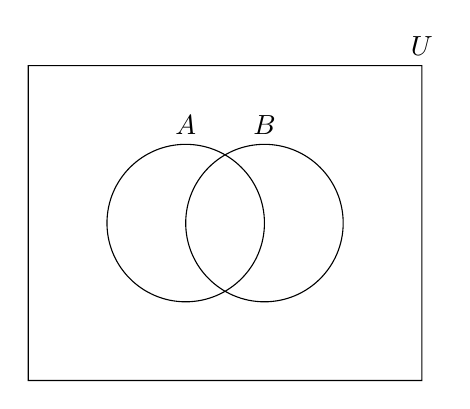
\begin{tikzpicture}[fill=white]
    \draw (0,0) circle (1) (0,1)  node [text=black,above] {$A$}
    (1,0) circle (1) (1,1)  node [text=black,above] {$B$}
    (-2,-2) rectangle (3,2) node [text=black,above] {$U$};
  \end{tikzpicture}
\end{center}

If $A \subseteq B$ and there is an element of $B$ that is not an element of $A$, meaning $A \not = B$,
then $A$ is a \textbf{proper subset} of $B$, denoted as $A \subset B$. An important fact is that
$\mathbb{N} \subset \mathbb{Z} \subset \mathbb{B} \subset \mathbb{R}$

\subsection{Sets of sets}

Elements of sets can be sets themselves, consider $A = \{\{1, 2\}, \emptyset, \{1, 2, 3\}, \{1\}\}$.
The cardinality of $A$ is 4, $\left\lvert A\right\rvert = 4$. Additionally, $\{1, 2\} \in A$, but
$1 \not \in A$.

The \textbf{Powerset} of A, denoted as $P(A)$ is the set of all subsets of $A$. For example,
\begin{align*}
  A    & = \{1, 2, 3\}                                                        \\
  P(A) & = \{\{1\}, \{2\}, \{3\}, \{1, 2\}, \{1, 3\}, \{2, 3\}, \{1, 2, 3\}\}
\end{align*}

\subsubsection*{Cardinality of a Powerset}

Let A be a finite set of cardinality $n$. Then the cardinality of the powerset of A is $2^n$.
\begin{align*}
  \left\lvert A\right\rvert    & = n   \\
  \left\lvert P(A)\right\rvert & = 2^n
\end{align*}

\subsection{Union and Intersection}

\textbf{Intersection} set operation: $\cap$.
$A$ intersected with $B$ is defined to be the set containing elements which are in both $A$ \underline{and} $B$.
That is, $A \cap B = \{x: x \in A \land x \in B\}$.
\begin{center}
  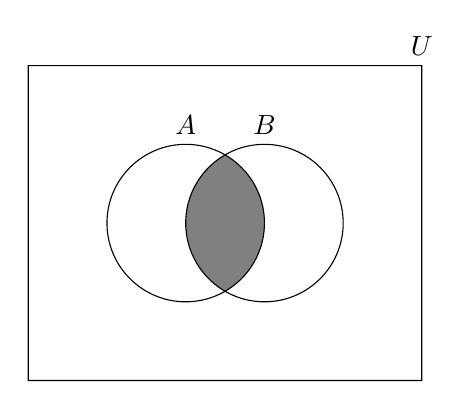
\begin{tikzpicture}
    \filldraw[fill=white] (-2,-2) rectangle (3,2);
    \scope % A \cap B
    \clip (0,0) circle (1);
    \fill[gray] (1,0) circle (1);
    \endscope
    % outline
    \draw (0,0) circle (1) (0,1)  node [text=black,above] {$A$}
    (1,0) circle (1) (1,1)  node [text=black,above] {$B$}
    (-2,-2) rectangle (3,2) node [text=black,above] {$U$};
  \end{tikzpicture}
\end{center}

Intersection $\cap$ can also apply to infinite sets:
\begin{align*}
  A        & =\{x \in \mathbb{Z}: x \text{ is an integer multiple of 2}\}  \\
  B        & =\{x \in \mathbb{Z}: x \text{ is an integer multiple of 3}\}  \\
  A \cap B & = \{x \in \mathbb{Z}: x \text{ is an integer multiple of 6}\}
\end{align*}

\noindent \textbf{Union} set operation $\cup$.
$A$ union with $B$ is defined to be the set containing elements which are in $A$ \underline{or} $B$.
That is, $A \cup B = \{x: x \in A \lor x \in B\}$.
\begin{center}
  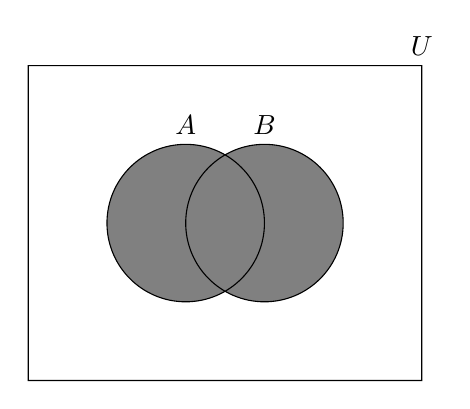
\begin{tikzpicture}
    \filldraw[fill=white] (-2,-2) rectangle (3,2);
    \fill[gray] (0,0) circle (1);
    \fill[gray] (1,0) circle (1);
    % outline
    \draw (0,0) circle (1) (0,1)  node [text=black,above] {$A$}
    (1,0) circle (1) (1,1)  node [text=black,above] {$B$}
    (-2,-2) rectangle (3,2) node [text=black,above] {$U$};
  \end{tikzpicture}
\end{center}

A special notation, similar to $\sum$ or $\prod$ notation, allows for compound representation of the
intersections or unions of a long sequence of sets.
\begin{align*}
  \bigcap_{i=1}^{n} A_{i} & = A_1 \cap A_2 \cap A_3 \cap \cdots \cap A_n = \{x : x \in A, \text{ for \underline{all} } 1 \leq i \leq n\}  \\
  \bigcup_{i=1}^{n} A_{i} & = A_1 \cup A_2 \cup A_3 \cup \cdots \cup A_n = \{x : x \in A, \text{ for \underline{some} } 1 \leq i \leq n\} \\
\end{align*}

Consider $A_j =$ a word with $j$ letters, with $U =$ is the Oxford English Dictionary.
\begin{align*}
  \bigcup_{j=1}^{10} A_j & = \text{ the set of all words with 10 letters or fewer in the OED} \\
  \bigcap_{j=1}^{45} A_j & = \emptyset                                                        \\
  \bigcup_{j=1}^{45} A_j & = \text{ the set of all words in the OED.}
\end{align*}

\subsection{More set operations}

\textbf{Difference} set operation $-$.
$A$ difference with $B$ is defined to be the set containing elements which are in $A$ but \underline{not} $B$.
That is, $A - B = \{x: x \in A \land x \not \in B\}$. A set difference is \underline{not} strictly commutative, often
$A - B \not = B - A$.
\begin{center}
  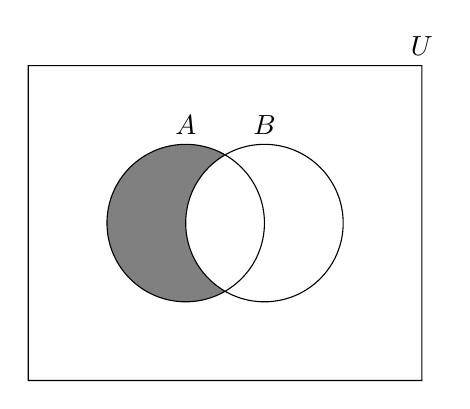
\begin{tikzpicture}[fill=gray]
    % left hand
    \scope
    \clip (-2,-2) rectangle (2,2)
    (1,0) circle (1);
    \fill (0,0) circle (1);
    \endscope
    % outline
    \draw (0,0) circle (1) (0,1)  node [text=black,above] {$A$}
    (1,0) circle (1) (1,1)  node [text=black,above] {$B$}
    (-2,-2) rectangle (3,2) node [text=black,above] {$U$};
  \end{tikzpicture}
\end{center}

\noindent \textbf{Symmetric Difference} set operation $\triangle$.
$A$ symmetric difference with $B$ is defined to be the set containing elements which are in $A$ or $B$, but not $A$ and $B$.
That is, $A \triangle B = \{x: x \in A \oplus  x \in B\}$.
\begin{center}
  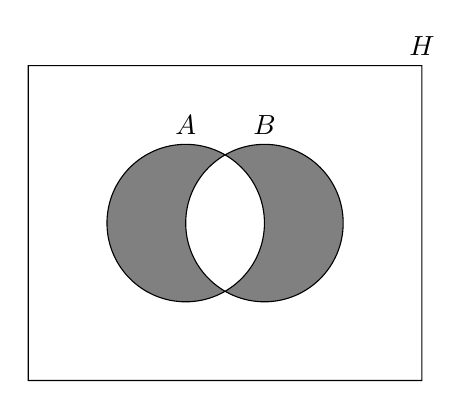
\begin{tikzpicture}[fill=gray]
    % left hand
    \scope
    \clip (-2,-2) rectangle (2,2)
    (1,0) circle (1);
    \fill (0,0) circle (1);
    \endscope
    % right hand
    \scope
    \clip (-2,-2) rectangle (2,2)
    (0,0) circle (1);
    \fill (1,0) circle (1);
    \endscope
    % outline
    \draw (0,0) circle (1) (0,1)  node [text=black,above] {$A$}
    (1,0) circle (1) (1,1)  node [text=black,above] {$B$}
    (-2,-2) rectangle (3,2) node [text=black,above] {$H$};
  \end{tikzpicture}
\end{center}

\noindent \textbf{Complement} set operation $\overline{ }$.
complement $A$ is defined to be the set containing elements in $U$ which are not in $A$.
That is, $\overline{A}= \{x: x \in U \land x \not \in A\}$.
\begin{center}
  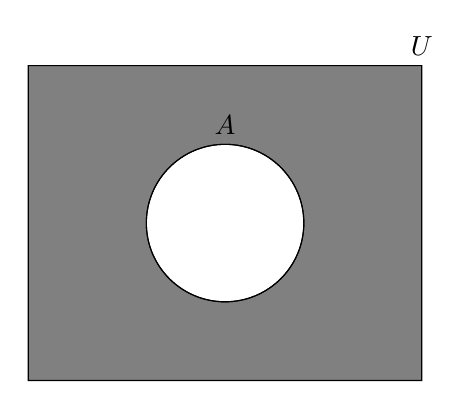
\begin{tikzpicture}[fill=white]
    \draw[fill=gray] (-2,-2) rectangle (3,2);
    \draw[fill=white] (0.5,0) circle (1);
    % outline
    \draw (0.5,0) circle (1) (0.5,1)  node [text=black,above] {$A$}
    (-2,-2) rectangle (3,2) node [text=black,above] {$U$};
  \end{tikzpicture}
\end{center}

\begin{center}
  \begin{tabular}{l|c|l}
    \multicolumn{3}{c}{\textbf{Summary of Set Operations}}                       \\
    Operation            & Notation        & Set Builder                         \\
    \hline
    Intersection         & $A \cap B$      & $\{x: x \in A \land x \in B\}$      \\
    Union                & $A \cup B$      & $\{x: x \in A \lor x \in B\}$       \\
    Difference           & $A - B$         & $\{x: x \in A \land x \not \in B\}$ \\
    Symmetric Difference & $A \triangle B$ & $\{x: x \in A \oplus  x \in B\}$    \\
    Complement           & $\overline{A}$  & $\{x: x \in U \land x \not \in A\}$ \\
  \end{tabular}
\end{center}

\subsection{Set identities}

The laws of propositional logic can be used to derive corresponding set identities.
A \textbf{set identity} is an equation involving sets that is true,
regardless of the contents of the sets used in the expression.
\begin{center}
  \begin{tabular}{r|c|c}
    \textbf{Law Name} & $\cup$ Union                                           & $\cap$ Intersection                                    \\
    \hline
    Idempotent        & $A \cup A = A$                                         & $A \cap A = A$                                         \\
    Associative       & $(A \cup B) \cup C = A \cup (B \cup C)$                & $(A \cap B) \cap C = A \cap (B \cap C)$                \\
    Commutative       & $A \cup B = B \cup A$                                  & $A \cap B = B \cap A$                                  \\
    Distributive      & $A \cup (B \cap C) = (A \cup B) \cap (A \cup C)$       & $A \cap (B \cup C) = (A \cap B) \cup (A \cap C)$       \\
    Identity          & $A \cup \emptyset = A$                                 & $A \cap U = A$                                         \\
    Domination        & $A \cup U = U$                                         & $A \cap \emptyset = \emptyset$                         \\
    Double Complement & $\overline{\overline{A}} = A$                                                                                   \\
    Complement        & $A \cup \overline{A} =$ T                              & $A \cap \overline{A} =$ F                              \\
    DeMorgan          & $\overline{A \cup B} = \overline{A} \cap \overline{B}$ & $\overline{A \cap B} = \overline{A} \cup \overline{B}$ \\
    Absorption        & $A \cup (A \cap B) = A$                                & $A \cap (A \cup B) = A$
  \end{tabular}
\end{center}

\subsection{Cartesian products}

An \textbf{ordered pair} of items is written $(x, y)$, where the first entry is $x$ and the second entry is $y$.
The use of $()$ instead of $\{\}$ indicates that order matters.

\noindent \textbf{Cartesian Product} of $A$ and $B$, $A \times B = \{(a, b) : a \in A \land b \in B\}$
\begin{align*}
  A & = \{1, 2\}    & A \times B & = \{(1, a), (1, b), (1, c), (2, a), (2, b), (2, c)\} \\
  B & = \{a, b, c\} & B \times A & = \{(a, 1), (a, 2), (b, 1), (b, 2), (c, 1), (c, 2)\}
\end{align*}

An ordered list of 3 items is called an \textbf{ordered triple}, denoted as $(x, y, z)$.
For a size of $\geq 4$, use the term \textbf{n-tuple}. For example, $(u, w, x, y, z)$.
\begin{align*}
  A_1 \times A_2 \times \cdots \times A_n = \{(a_1, a_2, \ldots, a_n) : a_i \in A \text{ for all $i$ such that} 1 \leq i \leq n\}
\end{align*}
Another Example
\begin{align*}
  A & = \{a, b\}          & (a, 1, y, \beta)  & \in A \times B \times C \times D      \\
  B & = \{1, 2\}          & (b, 1, x, \alpha) & \in A \times B \times C \times D      \\
  C & = \{x, y\}          & (1, b, x, \beta)  & \not \in A \times B \times C \times D \\
  D & = \{\alpha, \beta\} &                   & \text{order matters}
\end{align*}

$A \times A = A^2$, and in general,
\begin{align*}
  A^k = \underbrace{A \times A \times \cdots \times A}_{k-times}
\end{align*}
The \textbf{Cardinality of Cartesian Products}:
\begin{align*}
  \left\lvert A^n \right\rvert                           & = {\left\lvert A \right\rvert}^n                                               \\
  \left\lvert A_1 \times A_2 \times \cdots  \right\rvert & = \left\lvert A_1 \right\rvert \cdot \left\lvert A_2 \right\rvert \cdot \cdots
\end{align*}

\subsubsection*{Strings}

A sequence of characters is called a \textbf{string}.
The set of characters used in a set of string is called the \textbf{alphabet} for the set of strings.
The \textbf{length} of a string is the number of characters in the string.
For example, the length of $'xxyxyx'$ is $6$.
The \textbf{empty string} is a string whose length is $0$, and is usually denoted by $\lambda$.
It is useful for $A^0$, for some alphabet $A$. $\{0, 1\}^0 = \{\lambda\}$.
If $s$ and $t$ are two strings, then the \textbf{concatenation} of $s$ and $t$ is the string obtained by putting $s$ and $t$ together.
\begin{align*}
  s & = 010 & st & = 01011 \\
  t & = 11  & t0 & = 110
\end{align*}
Strings are used to specify passwords for computers or online accounts.
Security systems vary with respect to the alphabet of characters allowed or required in a valid password.
Strings also play an important rules in discrete mathematics as a mathematical tool to help count cardinality of sets.

\subsection{Partitions}

Two sets, $A$ and $B$, are said to be \textbf{disjoint} if their intersection is empty $(A \cap B = \emptyset)$.
A sequence of sets, $A_1, A_2, A_3, \ldots, A_n$, is \textbf{pairwise disjoint} if every pair of distinct sets in the sequence is disjoint.
A \textbf{partition} of a non-empty set $A$ is a collection of non-empty subsets such that each element of $A$ is in exactly one of the subsets.
$A_1, A_2, A_3, \ldots, A_n$ is a partition for a nonempty set $A$ if:
\begin{itemize}
  \item For all $i, A_i \subseteq A$
  \item For all $i, A_i \not = \emptyset$
  \item $A_1, A_2, \ldots, A_n$ are pairwise disjoint
  \item $A = \bigcup_{i=1}^{n} A_i$, for some $n \in \mathbb{Z}^+$
\end{itemize}
\begin{center}
  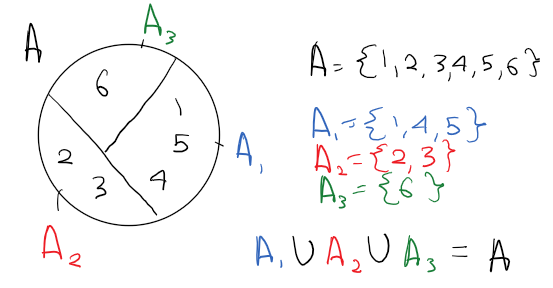
\includegraphics[width=.6\linewidth]{resources/partitions.png}
\end{center}
\section{Functions}
\subsection{Definition of functions}

A \textbf{function} maps elements of one set $X$ to elements of another set $Y$.
A function from $X$ to $Y$ can be viewed as a subset of $X \times Y : (x, y) \in f$ if $f$ maps $x$ to $y$.
The notation for a function is:
\[
  f: X \rightarrow Y \text{, where $X$ is the \textbf{domain} and $Y$ is the \textbf{co-domain}.}
\]

*if $f$ maps an element of the domain to zero elements \underline{or} more than one element of the target,
then $f$ is \underline{not} \textit{well-defined}

\textbf{Arrow Diagram}:
\begin{align*}
  X & = \{w, x, y, z\} \\
  Y & = \{a, b, c, d\}
\end{align*}

Well-defined functions:
\begin{center}
  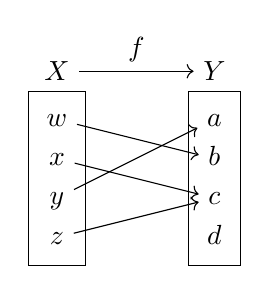
\begin{tikzpicture}
    \foreach[count=\i] \set/\elements in {X/{w,x,y,z}, Y/{a,b,c,d}} { %domain and co-domain
    \begin{scope}[local bounding box=\set, x=2cm, y=0.5cm]
      \foreach[count=\j] \element in \elements {
        \node[minimum width=1em,anchor=base,text height=1.4ex,text depth=0.25ex]
        (\i-\element) at (\i,-\j) {$\element$};
      }
    \end{scope}
    \node[draw, fit=(\set), label={[name=\i]above:$\set$}] {};
    }
    \foreach \domain/\target in {w/b,x/c,y/a,z/c} { %function pairs, uses indices
        \draw[->] (1-\domain) -- (2-\target);
      }
    \draw[->] (1) -- node[above]{$f$}(2); %function name
  \end{tikzpicture}
  \qquad
  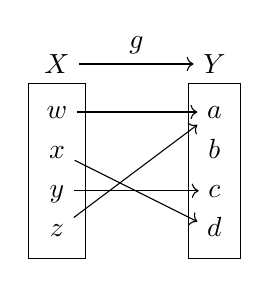
\begin{tikzpicture}
    \foreach[count=\i] \set/\elements in {X/{w,x,y,z}, Y/{a,b,c,d}} { %domain and co-domain
    \begin{scope}[local bounding box=\set, x=2cm, y=0.5cm]
      \foreach[count=\j] \element in \elements {
        \node[minimum width=1em,anchor=base,text height=1.4ex,text depth=0.25ex]
        (\i-\element) at (\i,-\j) {$\element$};
      }
    \end{scope}
    \node[draw, fit=(\set), label={[name=\i]above:$\set$}] {};
    }
    \foreach \domain/\target in {w/a,x/d,y/c,z/a} { %function pairs, uses indices
        \draw[->] (1-\domain) -- (2-\target);
      }
    \draw[->] (1) -- node[above]{$g$}(2); %function name
  \end{tikzpicture}
\end{center}

\underline{Not} well-defined functions:
\begin{center}
  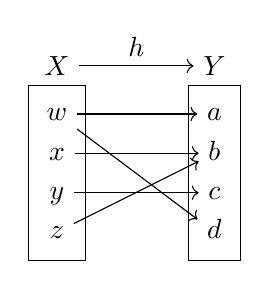
\begin{tikzpicture}
    \foreach[count=\i] \set/\elements in {X/{w,x,y,z}, Y/{a,b,c,d}} { %domain and co-domain
    \begin{scope}[local bounding box=\set, x=2cm, y=0.5cm]
      \foreach[count=\j] \element in \elements {
        \node[minimum width=1em,anchor=base,text height=1.4ex,text depth=0.25ex]
        (\i-\element) at (\i,-\j) {$\element$};
      }
    \end{scope}
    \node[draw, fit=(\set), label={[name=\i]above:$\set$}] {};
    }
    \foreach \domain/\target in {w/a,w/d,x/b,y/c,z/b} { %function pairs, uses indices
        \draw[->] (1-\domain) -- (2-\target);
      }
    \draw[->] (1) -- node[above]{$h$}(2); %function name
  \end{tikzpicture}
  \qquad
  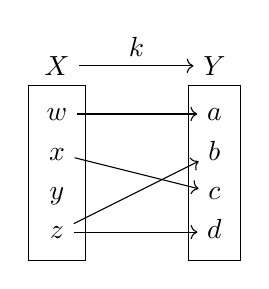
\begin{tikzpicture}
    \foreach[count=\i] \set/\elements in {X/{w,x,y,z}, Y/{a,b,c,d}} { %domain and co-domain
    \begin{scope}[local bounding box=\set, x=2cm, y=0.5cm]
      \foreach[count=\j] \element in \elements {
        \node[minimum width=1em,anchor=base,text height=1.4ex,text depth=0.25ex]
        (\i-\element) at (\i,-\j) {$\element$};
      }
    \end{scope}
    \node[draw, fit=(\set), label={[name=\i]above:$\set$}] {};
    }
    \foreach \domain/\target in {w/a,x/c,z/b,z/d} { %function pairs, uses indices
        \draw[->] (1-\domain) -- (2-\target);
      }
    \draw[->] (1) -- node[above]{$k$}(2); %function name
  \end{tikzpicture}
\end{center}

For function $f: X \rightarrow Y$, an element $y$ is in the \textbf{range} of $f$
iff there is an $x \in X$ such that $(x, y) \in f$.
\[
  \text{Range of } f = \{y : (x, y) \in f, \text{ for some } x \in X\}
\]
Two functions, $f$ and $g$, are \textbf{equal} if $f$ and $g$ have the same domain and target and
$f(x) = g(x)$ for \underline{every} $x$ in the domain.
\[
  \forall~ x : f(x) = g(x) \implies f = g
\]

\subsection{Floor and Ceiling functions}

The \textbf{Floor} function, $\left\lfloor x\right\rfloor$
\[
  \text{floor}: \mathbb{R} \rightarrow \mathbb{Z}, \text{ where floor$(x)$ = the largest integer $y$ such that $y \leq x$.}
\]
Notation: $\text{floor}(x) = \left\lfloor x\right\rfloor$
\[\]
\noindent The \textbf{Ceiling} function, $\left\lceil x\right\rceil$
\[
  \text{ceiling}: \mathbb{R} \rightarrow \mathbb{Z}, \text{ where ceiling$(x)$ = the smallest integer $y$ such that $y \geq x$.}
\]
Notation: $\text{ceiling}(x) = \left\lceil x\right\rceil$

\noindent Examples of floor and ceiling:
\begin{align*}
  \left\lceil 4.32\right\rceil  & = 5  & \left\lfloor 4.32\right\rfloor  & = 4  \\
  \left\lceil -4.32\right\rceil & = -4 & \left\lfloor -4.32\right\rfloor & = -5 \\
  \left\lceil 4\right\rceil     & = 4  & \left\lfloor 4\right\rfloor     & = 4  \\
  \left\lceil -4\right\rceil    & = -4 & \left\lfloor -4\right\rfloor    & = -4 \\
\end{align*}

\subsection{Properties of functions}

A function $f: X \rightarrow Y$ is \textbf{one-to-one} or \textbf{injective} if $x_1 \not = x_2$ implies that $f(x_1) \not = f(x_2)$.
$f$ maps different elements in x to different elements in y.

A function $f: X \rightarrow Y$ is \textbf{onto} or \textbf{surjective} if the range of $f$ is equal to the target $Y$.
That is, $\forall~ y \exists~ x (y \in Y \land x \in X \land f(x) = y)$

A function $f: X \rightarrow Y$ is \textbf{bijective} if it is both \textbf{injective} and \textbf{surjective}.
A \textbf{bijective} function is called a \textbf{bijection}, or a \textbf{one-to-one correspondence}.

When the domain and target are finite sets, it is possible to infer information about their relative sizes
based on whether a function is one-to-one or onto.
\begin{align*}
  f: D \rightarrow T & \text{ is \textbf{one-to-one}} & \implies &  & \left\lvert D\right\rvert & \leq \left\lvert T\right\rvert \\
  f: D \rightarrow T & \text{ is \textbf{onto}}       & \implies &  & \left\lvert D\right\rvert & \geq \left\lvert T\right\rvert \\
  f: D \rightarrow T & \text{ is \textbf{bijective}}  & \implies &  & \left\lvert D\right\rvert & = \left\lvert T\right\rvert
\end{align*}

\subsection{The inverse of a function}

If a function $f: X \rightarrow Y$ is a \textit{bijection},
then the \textbf{inverse} of f is obtained by exchanging the first and second entries in each pair in $f$.
\begin{align*}
  \text{given } f        & : X \rightarrow Y           \\
  \text{inverse } f^{-1} & : \{(y, x) : (x, y) \in f\}
\end{align*}
Reversing the cartesian pair does not always create a well-defined function.
\textit{Some functions do not have an inverse}.

\textbf{Examples}:
\begin{align*}
  X & = \{1, 2, 3\} & f = \{(1, 7), (2, 9), (3, 9)\} \\
  Y & = \{7, 8, 9\} & g = \{(1, 9), (2, 7), (3, 8)\}
\end{align*}

\begin{center}
  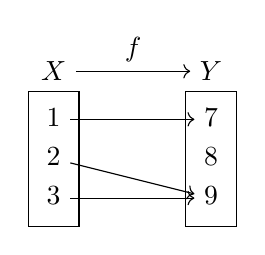
\begin{tikzpicture}
    \foreach[count=\i] \set/\elements in {X/{1,2,3}, Y/{7,8,9}} { %domain and co-domain
    \begin{scope}[local bounding box=\set, x=2cm, y=0.5cm]
      \foreach[count=\j] \element in \elements {
        \node[minimum width=1em,anchor=base,text height=1.4ex,text depth=0.25ex]
        (\i-\element) at (\i,-\j) {$\element$};
      }
    \end{scope}
    \node[draw, fit=(\set), label={[name=\i]above:$\set$}] {};
    }
    \foreach \domain/\target in {1/7,2/9,3/9} { %function pairs, uses indices
        \draw[->] (1-\domain) -- (2-\target);
      }
    \draw[->] (1) -- node[above]{$f$}(2); %function name
  \end{tikzpicture}
  \qquad
  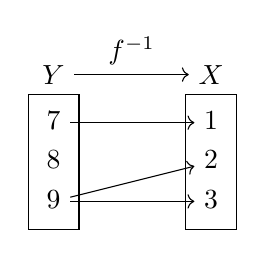
\begin{tikzpicture}
    \foreach[count=\i] \set/\elements in {Y/{7,8,9}, X/{1,2,3}} { %domain and co-domain
    \begin{scope}[local bounding box=\set, x=2cm, y=0.5cm]
      \foreach[count=\j] \element in \elements {
        \node[minimum width=1em,anchor=base,text height=1.4ex,text depth=0.25ex]
        (\i-\element) at (\i,-\j) {$\element$};
      }
    \end{scope}
    \node[draw, fit=(\set), label={[name=\i]above:$\set$}] {};
    }
    \foreach \domain/\target in {7/1,9/2,9/3} { %function pairs, uses indices
        \draw[->] (1-\domain) -- (2-\target);
      }
    \draw[->] (1) -- node[above]{$f^{-1}$}(2); %function name
  \end{tikzpicture}

  $f^{-1}$ is not well defined, therefore $f$ does not have an inverse.
\end{center}
\begin{center}
  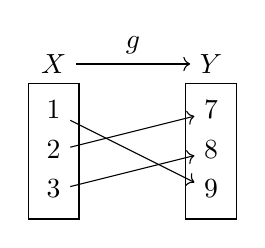
\begin{tikzpicture}
    \foreach[count=\i] \set/\elements in {X/{1,2,3}, Y/{7,8,9}} { %domain and co-domain
    \begin{scope}[local bounding box=\set, x=2cm, y=0.5cm]
      \foreach[count=\j] \element in \elements {
        \node[minimum width=1em,anchor=base,text height=1.4ex,text depth=0.25ex]
        (\i-\element) at (\i,-\j) {$\element$};
      }
    \end{scope}
    \node[draw, fit=(\set), label={[name=\i]above:$\set$}] {};
    }
    \foreach \domain/\target in {1/9,2/7,3/8} { %function pairs, uses indices
        \draw[->] (1-\domain) -- (2-\target);
      }
    \draw[->] (1) -- node[above]{$g$}(2); %function name
  \end{tikzpicture}
  \qquad
  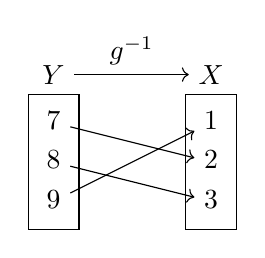
\begin{tikzpicture}
    \foreach[count=\i] \set/\elements in {Y/{7,8,9}, X/{1,2,3}} { %domain and co-domain
    \begin{scope}[local bounding box=\set, x=2cm, y=0.5cm]
      \foreach[count=\j] \element in \elements {
        \node[minimum width=1em,anchor=base,text height=1.4ex,text depth=0.25ex]
        (\i-\element) at (\i,-\j) {$\element$};
      }
    \end{scope}
    \node[draw, fit=(\set), label={[name=\i]above:$\set$}] {};
    }
    \foreach \domain/\target in {9/1,7/2,8/3} { %function pairs, uses indices
        \draw[->] (1-\domain) -- (2-\target);
      }
    \draw[->] (1) -- node[above]{$g^{-1}$}(2); %function name
  \end{tikzpicture}

  $g^{-1}$ is well defined, therefore $g$ does have an inverse.
\end{center}

\subsection{Composition of functions}

The process of applying a function to the result of another function is called \textbf{composition}.
\begin{align*}
  f           & : X \rightarrow Y                                                                   \\
  g           & : Y \rightarrow Z                                                                   \\
  (g \circ f) & : X \rightarrow Z, \text{ such that } \forall~ x : x \in X, (g \circ f)(x) = g(f(x))
\end{align*}
Remember that order matters, as often $(g \circ f)(x) \not = (f \circ g)(x)$. However, composition is associative:
\[
  (f \circ g \circ h)(x) = ((f \circ g) \circ h)(x) = (f \circ (g \circ h))(x) = f(g(h(x)))
\]

\subsubsection*{Identity Function}

The \textbf{Identity Function} maps a set onto itself and maps every element to itself. It is notated as $I_A: A \rightarrow A$,
where $A$ is the set it maps. There are a number of identities about the Identity Function.

Let $f: A \rightarrow B$ be a bijection. Then,
\[
  f \circ f^{-1} = I_B \text{ and } f^{-1} \circ f = I_A
\]

\subsection{Logarithms and exponents}

The \textbf{Exponential} function, $\text{exp}_b: \mathbb{R} \rightarrow \mathbb{R}^+, \text{exp}_b(x) = b^x$.
$b$ is the base of the exponent and $x$ is the exponent.

Properties of exponents:
\begin{align*}
  b^{x}b^{y}      & = b^{x+y} & b & \in \mathbb{R}^+ & c & \in \mathbb{R}^+ \\
  (b^x)^{y}       & = b^{xy}  & x & \in \mathbb{R}   & y & \in \mathbb{R}   \\
  \frac{b^x}{b^y} & = b^{x-y}                                               \\
  (bc)^x          & = b^xc^x
\end{align*}

\begin{center}
  \begin{tikzpicture}
    \draw[<->] (-3,0) -- (3,0) node[right] {$x$};
    \draw[<->] (0,-3) -- (0,3) node[above] {$y$};
    \begin{scope}
      \clip (-3,-3) rectangle (3,3);
      \draw[domain=-3:3, variable=\x, samples=50, smooth, blue, thick] plot ({\x}, {(exp(\x))});
    \end{scope}
    \begin{scope}
      \clip (-3,-3) rectangle (3,3);
      \draw[domain=0.0001:3, variable=\x, samples=50, smooth, red, thick] plot ({\x}, {(ln(\x))});
    \end{scope}
    \draw (-1,-1) node[red] {log$(x)$};
    \draw (2,2) node[blue] {exp$(x)$};
  \end{tikzpicture}
\end{center}

The \textbf{Logarithms} function, $\text{log}_b: \mathbb{R} \rightarrow \mathbb{R}^+, \text{log}_b(y) = x$.
$b$ is the base of the logarithm and $x$ is the exponent.

Properties of exponents:
\begin{align*}
  \text{log}_b(xy)          & = \text{log}_bx + \text{log}_by       & b & \in \mathbb{R}^+ \\
  \text{log}_b(\frac{x}{y}) & = \text{log}_bx - \text{log}_by       & c & \in \mathbb{R}^+ \\
  \text{log}_b(x^y)         & = y\text{log}_bx                      & x & \in \mathbb{R}   \\
  \text{log}_cx             & = \frac{\text{log}_bx}{\text{log}_bc} & y & \in \mathbb{R}
\end{align*}
\section{Boolean Algebra}
\subsection{An introduction to Boolean Algebra}

\textbf{Boolean Algebra} is a set of rules/operations for working with variables whose values are either 0 or 1.
It corresponds highly to propositional logic.

\textbf{Boolean Multiplication}, denoted by $\cdot$
\begin{align*}
  \text{Boolean } & \cdot & \text{Logic }           & \land      \\
  0 \cdot 0       & = 0   & \text{F} \land \text{F} & = \text{F} \\
  0 \cdot 1       & = 0   & \text{F} \land \text{T} & = \text{F} \\
  1 \cdot 0       & = 0   & \text{T} \land \text{F} & = \text{F} \\
  1 \cdot 1       & = 1   & \text{T} \land \text{T} & = \text{T}
\end{align*}

\textbf{Boolean Addition}, denoted by $+$
\begin{align*}
  \text{Boolean } & \cdot & \text{Logic }          & \lor       \\
  0 + 0           & = 0   & \text{F} \lor \text{F} & = \text{F} \\
  0 + 1           & = 1   & \text{F} \lor \text{T} & = \text{T} \\
  1 + 0           & = 1   & \text{T} \lor \text{F} & = \text{T} \\
  1 + 1           & = 1   & \text{T} \lor \text{T} & = \text{T} \\
\end{align*}

\textbf{Boolean Complement}, denoted by $\bar{ }$
\begin{align*}
  \text{Boolean } & \bar{ } & \text{Logic }  & \lnot      \\
  \bar{0}         & = 1     & \lnot \text{F} & = \text{T} \\
  \bar{1}         & = 0     & \lnot \text{T} & = \text{F} \\
\end{align*}

\begin{center}
  \begin{circuitikz}
    \draw (0,0) to[battery] (0,2)
    to[switch, l=$x$] (2,2)
    to[switch, l=$y$] (4,2)
    to[lamp] (4,0) -- (0,0);
    \draw (2,-1) node[] {Shannon Circuit (AND $\cdot$)};
  \end{circuitikz}
  \qquad
  \begin{circuitikz}
    \draw (0,0) to[battery] (0,2) -- (1,2) -- (1,1.5)
    to[switch, l=$x$] (3,1.5) -- (3,2) -- (4,2) to[lamp] (4,0) -- (0,0)
    (1,2) -- (1,2.5)
    to[switch, l=$y$] (3,2.5) -- (3,2);
    \draw (2,-1) node[] {Switching Circuit (OR $+$)};
  \end{circuitikz}
\end{center}

Variables that can have a value of either $1$ or $0$ are called \textbf{Boolean Variables}.
Boolean expressions are made of boolean variables. There are also common shorthand ways of notating operations.
\begin{align*}
  x \cdot y + 1 \cdot \bar{z} & = xy + \bar{z}        \\
  x + z + \overline{0 + y}    & = x + z \cdot \bar{y}
\end{align*}

\begin{center}
  \begin{tabular}{r|c|c}
    \textbf{Law Name} & $+$ OR                                               & $\cdot$ AND                                          \\
    \hline
    Idempotent        & $x + x = x$                                          & $x \cdot x = x$                                      \\
    Associative       & $(x + y) + z = x + (y + z)$                          & $(x \cdot y) \cdot z = x \cdot (y \cdot z)$          \\
    Commutative       & $x + y = y + x$                                      & $x \cdot y = y \cdot x$                              \\
    Distributive      & $x + (y \cdot z) = (x + y) \cdot (x + z)$            & $x \cdot (y + z) = (x \cdot y) + (x \cdot z)$        \\
    Identity          & $x + 0 = x$                                          & $x \cdot 1 = x$                                      \\
    Domination        & $x + 1 = 1$                                          & $x \cdot 0 = 0$                                      \\
    Double Complement & $\overline{\overline{x}} = x$                                                                               \\
    Complement        & $x + \overline{x} =$ 1                               & $x \cdot \overline{x} =$ 0                           \\
    DeMorgan          & $\overline{x + y} = \overline{x} \cdot \overline{y}$ & $\overline{x \cdot y} = \overline{x} + \overline{y}$ \\
    Absorption        & $x + (x \cdot y) = x$                                & $x \cdot (x + y) = x$
  \end{tabular}
\end{center}

\subsection{Boolean functions}

A \textbf{boolean function} is a function which maps $B^k \rightarrow B$,
where $B = \{0,1\}$. For example, consider $f:B^3 \rightarrow B$

\begin{center}
  \begin{tabular}{ccc|c}
    $x$ & $y$ & $z$ & $f(x, y, z)$ \\
    \hline
    0   & 0   & 0   & 0            \\
    0   & 0   & 1   & 0            \\
    0   & 1   & 0   & 0            \\
    0   & 1   & 1   & 1            \\
    1   & 0   & 0   & 1            \\
    1   & 0   & 1   & 1            \\
    1   & 1   & 0   & 0            \\
    1   & 1   & 1   & 1
  \end{tabular}
  \qquad
  \begin{tabular}{ccc|cc}
    $x$ & $y$ & $z$ & $f(x, y, z)$                     \\
    \hline
    0   & 0   & 0   & 0            &                   \\
    0   & 0   & 1   & 0            &                   \\
    0   & 1   & 0   & 0            &                   \\
    0   & 1   & 1   & 1            & $\bar{x}yz$       \\
    1   & 0   & 0   & 1            & $x\bar{y}\bar{z}$ \\
    1   & 0   & 1   & 1            & $x\bar{y}z$       \\
    1   & 1   & 0   & 0            &                   \\
    1   & 1   & 1   & 1            & $xyz$
  \end{tabular}
\end{center}
This function is equivalent to $f(x,y,z) = x \overline{y} + yz$.
This can be determined using the boolean table and a strategy of combining the cases.
\begin{align*}
  f(x,y,z) & = \bar{x}yz + x\bar{y}\bar{z} + x\bar{y}z + xyz \\
           & = y(\bar{x}z + xz) + \bar{y}(x\bar{z} + xz)     \\
           & = y(z \cdot 1) + \bar{y}(x \cdot 1)             \\
           & = yz + \bar{y}x = \bar{y}x + yz                 \\
           & = x\bar{y} + yz
\end{align*}

A \textbf{literal} is a boolean variable or the complement of a boolean variable,
for example $x$ or $\bar{x}$. In a boolean function whose input variables are
$v_1, v_2, \ldots, v_k$, a \textit{mini-term} is a product of literals
$u_1, u_2, \ldots, u_k$, such that $u_j$ is either $v_j$ or $\overline{v_j}$

\subsection{Disjunctive and conjunctive normal form}

A boolean expression that is the sum of literals is said to be in \textit{disjunctive normal form},
\textbf{DNF}. It has the following form:
\[
  c_1 + c_2 + \cdots + c_m, \text{ where $c_j$ for $j \in \{1,\ldots,m\}$ is a product of literals.}
\]
For example, $\bar{x}y\bar{z} + xy + w + y\bar{z}w$. The complement only applies to a single variable and
\underline{no} addition within a term.

A boolean expression that is the product of sums of literals is said to be in \textit{conjunctive normal form},
\textbf{CNF}. It has the following form:
\[
  d_1 \cdot d_2 \cdots d_m, \text{ where $d_j$ for $j \in \{1,\ldots,m\}$ is a sum of literals.} \\
\]
Each $d_j$ is called a clause, and complements are only applied to a single variable.
Additionally, there is no multiplication within variables.
An example is $(\bar{x} + y + z)(x + \bar{y})(w)(y + \bar{z} + w)$.

\subsection{Functional completeness}

A set of operators is functionally complete if any boolean function can be expressed using only operations from the set.
Two expressions can be added using only multiplication and complement.
\[
  x + y = \overline{\bar{x} \bar{y}} \text{ DeMorgan's Law}
\]
DeMorgan's Law can be extended to more than two boolean variables:
\[
  x + y + w + z = \overline{\bar{x} \bar{y} \bar{w} \bar{z}}
\]
The same can be said about the addition variant of the law:
\begin{align*}
  xy   & = \overline{\bar{x} + \bar{y}}                     \\
  xywz & = \overline{\bar{x} + \bar{y} + \bar{w} + \bar{z}}
\end{align*}

The \textbf{NAND} operation, $\uparrow$, and the \textbf{NOR} operation, $\downarrow$.
\begin{center}
  \begin{tabular}{cc|cc}
    $x$ & $y$ & $x \uparrow y$ & $x \downarrow y$ \\
    \hline
    0   & 0   & 1              & 1                \\
    0   & 1   & 1              & 0                \\
    1   & 0   & 1              & 0                \\
    1   & 1   & 0              & 0
  \end{tabular}
\end{center}

$\{\text{NAND}\}$ is functionally complete, it can create the complement,
from which all other possible gates can be created.
\begin{center}
  \begin{tabular}{c|c}
    $x$ & $x \uparrow x$ \\
    \hline
    0   & 1              \\
    1   & 0
  \end{tabular}
\end{center}
From the complement, AND can be created, and \{AND, COMPLEMENT\} has already been proven to be functionally complete.
\[
  xy = \overline{x \uparrow y} = (x \uparrow y) \uparrow (x \uparrow y)
\]

\subsection{Boolean satisfiability}

The \textbf{Boolean Satisfiability problem}, called the \textit{SAT} for short,
takes the boolean expression as an input and asks whether it is possible to set the values of the variables
so that the expression evaluates to 1.
\begin{align*}
  \text{If } & \exists~ x \exists~ y \ldots B(x, y, \ldots), \text{ then the expression is \textbf{satisfiable}}         \\
  \text{If } & \forall~ x \forall~ y \ldots \lnot B(x, y, \ldots), \text{ then the expression is \textbf{unsatisfiable}} \\
\end{align*}
Expressions in DNF form are very easy to determine satisfiability.
If there is \underline{any} term which does \textit{not} contain a variable and its complement,
it is satisfiable. For example,
\[
  x\bar{y}z\bar{x} + \overbrace{\bar{w}xy\bar{z}}^\text{no self-complements} + \bar{w}xw\bar{x} + xy\bar{z}z
\]
The above equation \textit{is} satisfiable because there is a term which does not contain a self-complement.

\subsection{Gates and circuits}

Circuits are built from electrical devices called \textbf{gates}.
\begin{center}
  \textbf{AND}:
  \begin{circuitikz}
    \draw (0,0) node[and port] (AND){}
    (AND.in 1) node[anchor=east] {$x$}
    (AND.in 2) node[anchor=east] {$y$}
    (AND.out) node[anchor=west] {$xy$};
  \end{circuitikz}
  \quad
  \textbf{OR}:
  \begin{circuitikz}
    \draw (0,0) node[or port] (OR){}
    (OR.in 1) node[anchor=east] {$x$}
    (OR.in 2) node[anchor=east] {$y$}
    (OR.out) node[anchor=west] {$x+y$};
  \end{circuitikz}
  \quad
  \textbf{NOT/INVERTER}:
  \begin{circuitikz}
    \draw (0,0) node[not port] (NOT){}
    (NOT.in) node[anchor=east] {$x$}
    (NOT.out) node[anchor=west] {$\bar{x}$};
  \end{circuitikz}
\end{center}

The boolean function $f(x_1,x_2): (f(x_1,x_2) \cdot x_1) + x_2$. Yes, circuits can contain recursion.
\begin{center}
  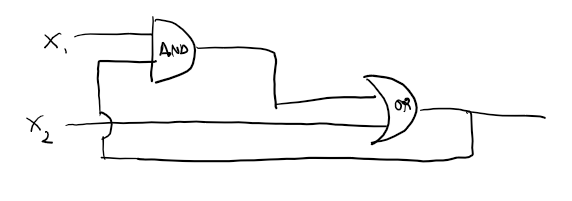
\includegraphics[width=.6\linewidth]{resources/recursive.png}
\end{center}

Boolean expressions can also be constructed by following the logic or a circuit.
\begin{center}
  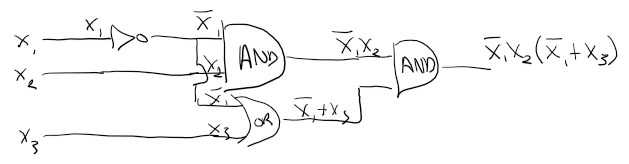
\includegraphics[width=.6\linewidth]{resources/construction_from_circuit.png}
\end{center}
\[
  f(x_1,x_2,x_3) = \bar{x}_1 x_2 (\bar{x}_1 + x_3)
\]

An example of constructing a circuit from a boolean expression, $f(x,y,z):(x+y)(\bar{z}+\bar{y})$
\begin{center}
  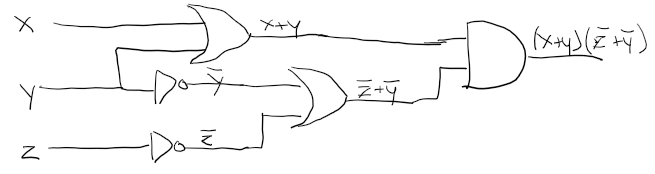
\includegraphics[width=.6\linewidth]{resources/construction_from_function.png}
\end{center}

\subsubsection*{Designing Circuits}

\begin{enumerate}
  \item Build an input/output table with the desired output for every combination of input
  \item Construct a boolean expression that computes the same function as the function specified in the input/output table
  \item Construct a digital circuit that realizes the boolean expression
\end{enumerate}

I/O for sum of two bits, $x,y$
\begin{center}
  \begin{tabular}{cccc}
    x & y & m & l \\
    \hline
    0 & 0 & 0 & 0 \\
    1 & 0 & 0 & 1 \\
    0 & 1 & 0 & 1 \\
    1 & 1 & 1 & 0 \\
  \end{tabular}
\end{center}
\begin{align*}
  m & = xy                  & \text{most significant bit}  \\
  l & = x\bar{y} + \bar{x}y & \text{least significant bit}
\end{align*}
\begin{center}
  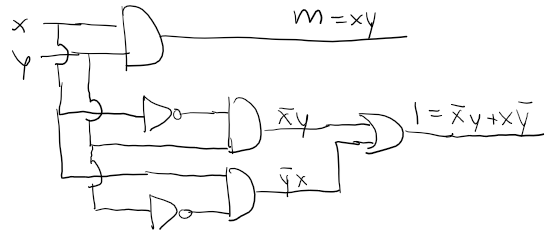
\includegraphics[width=.6\linewidth]{resources/sum_of_two_bits.png}
\end{center}
\begin{center}
  *\textit{this method does not necessarily give the most \underline{efficient} circuit}.
\end{center}
Circuits with fewer gates cost less to manufacture. Here is a simplified circuit to add two bits:
\begin{center}
  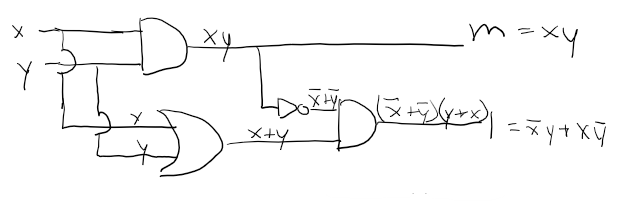
\includegraphics[width=.6\linewidth]{resources/better_sum_of_two_bits.png}
\end{center}

Here is another example with boolean logic for light switches:
\begin{center}
  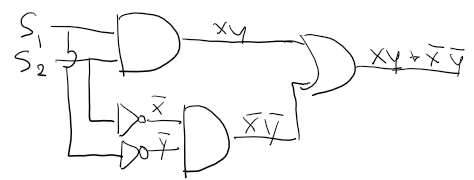
\includegraphics[width=.6\linewidth]{resources/switches.png}
\end{center}
\section{Relation and Digraphs}
\subsection{Introduction to binary relations}

A \textbf{Binary Relation} between two sets $A$ and $B$ is a subset $R$ of $A \times B$.
It is binary because it is between two sets.
\[
  \text{for } a \in A \land b \in B, (a,b) \in R \text{ is denoted as } a\text{R}b
\]

For example, consider the relation C between $\mathbb{R}$ and $\mathbb{Z}$:
\[
  x\text{C}y \text{ if } \left\lvert x-y\right\rvert \leq 1, \text{ where } x \in \mathbb{R} \text{ and } y \in \mathbb{Z}
\]
If $A$ and $B$ are finite, then relation R between $A$ and $B$ can be represented by a set of ordered pairs.

\subsubsection*{Matrix Representation}
\begin{align*}
  P           & = \{\text{Sue}, \text{Harry}, \text{Sam}\}                       \\
  \text{File} & = \{\text{File A}, \text{File B}, \text{File C}, \text{File D}\}
\end{align*}
\[
  \bordermatrix{ & \text{File A} & \text{File B} & \text{File C} & \text{File D} \cr
    \text{Sue}   & 0 & 1 & 1 & 1 \cr
    \text{Harry} & 1 & 0 & 0 & 0 \cr
    \text{Sam}   & 0 & 0 & 0 & 0 \cr }
\]
\begin{center}
  An element is
  \begin{tabular}{c}
    1 if $p$R$f$ is true \\
    0 if $p$R$f$ is false
  \end{tabular}
\end{center}

\subsubsection*{Arrow Diagram}
\begin{align*}
  A & = \{a,b,c,d,e\}                                \\
  R & \subseteq A \times A                           \\
  R & = \{(a,b), (b,c), (e,c), (c,e), (d,a), (d,d)\}
\end{align*}
\begin{center}
  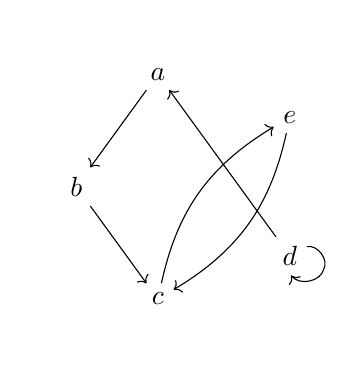
\begin{tikzpicture}
    %VARIABLES
    \pgfmathsetmacro{\gsize}{1.5}
    \pgfmathsetmacro{\gnum}{5}

    \foreach[count=\i] \element in {a,b,c,d,e} { %domain
        \node (\element) at (\i * 360 / \gnum + 180 / \gnum:\gsize) {$\element$};
        \node (\element-) at (\i * 360 / \gnum + 180 / \gnum:\gsize + 0.5) {};
      }
    \foreach \j/\l in {a/b,b/c,d/a} { %a to b
        \draw[->] (\j) -- (\l);
      }
    \foreach \j/\l in {e/c} { %a to b AND b to a
        \draw[->] (\j) to[bend left=20 / \gsize + 10] (\l);
        \draw[->] (\l) to[bend left=20 / \gsize + 10] (\j);
      }
    \foreach \j in {d} { %a to a
        \draw[->] (\j) to[bend left=65] (\j-)
        to[bend left=65] (\j);
      }
  \end{tikzpicture}
\end{center}

\subsubsection*{Arrow Diagram vs. Matrix Representation}
\begin{align*}
  A & = \{1,2,3,4\}                                  \\
  R & = \{(1,2), (1,3), (2,2), (2,3), (3,4), (4,3)\}
\end{align*}
\begin{center}
  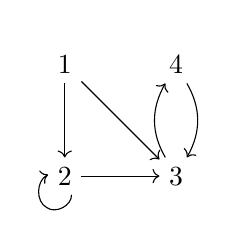
\begin{tikzpicture}
    %VARIABLES
    \pgfmathsetmacro{\gsize}{1}
    \pgfmathsetmacro{\gnum}{4}

    \foreach[count=\i] \element in {1,2,3,4} { %domain
        \node (\element) at (\i * 360 / \gnum + 180 / \gnum:\gsize) {$\element$};
        \node (\element-) at (\i * 360 / \gnum + 180 / \gnum:\gsize + 0.5) {};
      }
    \foreach \j/\l in {1/2,1/3,2/3} { %a to b
        \draw[->] (\j) -- (\l);
      }
    \foreach \j/\l in {3/4} { %a to b AND b to a
        \draw[->] (\j) to[bend left=20 / \gsize + 10] (\l);
        \draw[->] (\l) to[bend left=20 / \gsize + 10] (\j);
      }
    \foreach \j in {2} { %a to a
        \draw[->] (\j) to[bend left=65] (\j-)
        to[bend left=65] (\j);
      }
  \end{tikzpicture}
  \qquad
  $
    \bordermatrix{ & 1 & 2 & 3 & 4 \cr
      1 & 0 & 1 & 1 & 0 \cr
      2 & 0 & 1 & 1 & 0 \cr
      3 & 0 & 0 & 0 & 1 \cr
      4 & 0 & 0 & 1 & 0 \cr }
  $
\end{center}

\subsection{Properties of binary relations}

A binary relation of R on set $A$ is \textbf{Reflective} if for \textit{every} $x \in A$, $x$R$x$.
For Arrow Diagrams, this means the graph contains self-loops:
\begin{center}
  \begin{tikzpicture}
    %VARIABLES
    \pgfmathsetmacro{\gsize}{1}
    \pgfmathsetmacro{\gnum}{2}

    \foreach[count=\i] \element in {a,b} { %domain
        \node (\element) at (\i * 360 / \gnum:\gsize) {$\element$};
        \node (\element-) at (\i * 360 / \gnum:\gsize + 0.5) {};
      }
    \foreach \j in {a,b} { %a to a
        \draw[->] (\j) to[bend left=65] (\j-)
        to[bend left=65] (\j);
      }
  \end{tikzpicture}
\end{center}
For Matrix Representation, this means that the top left to bottom right diagonal are all 1's:
\[
  \bordermatrix{ & a & b & c & d \cr
    a & 1 & - & - & - \cr
    b & - & 1 & - & - \cr
    c & - & - & 1 & - \cr
    d & - & - & - & 1 \cr }
\]

A binary relation of R on set $A$ is \textbf{Anti-reflective} if for \textit{every} $x \in A$, $x$R$x$ is \textit{not} true.
For Arrow Diagrams, this means the graph does not contain self-loops:
\begin{center}
  \begin{tikzpicture}
    %VARIABLES
    \pgfmathsetmacro{\gsize}{1}
    \pgfmathsetmacro{\gnum}{2}

    \foreach[count=\i] \element in {a,b} { %domain
        \node (\element) at (\i * 360 / \gnum:\gsize) {$\element$};
        \node (\element-) at (\i * 360 / \gnum:\gsize + 0.5) {};
      }
  \end{tikzpicture}
\end{center}
For Matrix Representation, this means that the top left to bottom right diagonal are all 0's:
\[
  \bordermatrix{ & a & b & c & d \cr
    a & 0 & - & - & - \cr
    b & - & 0 & - & - \cr
    c & - & - & 0 & - \cr
    d & - & - & - & 0 \cr }
\]

A binary relation of R on set $A$ is \textbf{Symmetric} if and only if for \textit{every} pair $x \in A$, $y \in Y$,
either \textit{both} $x$R$y$ \underline{and} $y$R$x$, or \textit{both} not $x$R$y$ or not $y$R$x$ is true.
For Arrow Diagrams, this means that every arrow has an arrow going the other way:
\begin{center}
  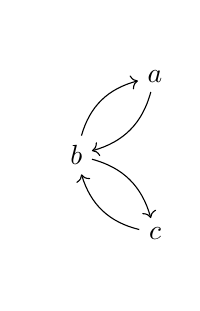
\begin{tikzpicture}
    %VARIABLES
    \pgfmathsetmacro{\gsize}{1}
    \pgfmathsetmacro{\gnum}{4}

    \foreach[count=\i] \element in {a,b,c} { %domain
        \node (\element) at (\i * 360 / \gnum:\gsize) {$\element$};
        \node (\element-) at (\i * 360 / \gnum:\gsize + 0.5) {};
      }
    \foreach \j/\l in {a/b,b/c} { %a to b AND b to a
        \draw[->] (\j) to[bend left=20 / \gsize + 10] (\l);
        \draw[->] (\l) to[bend left=20 / \gsize + 10] (\j);
      }
  \end{tikzpicture}
\end{center}
For Matrix Representation, this means that the matrix is symmetric along the top left to bottom right diagonal:
\begin{center}
  $
    \bordermatrix{ & a & b & c & d \cr
      a & - & u & v & x \cr
      b & u & - & w & y \cr
      c & v & w & - & z \cr
      d & x & y & z & - \cr }
  $
  where
  \begin{tabular}{c}
    $u \in \{0,1\}$ \\
    $\vdots$        \\
    $z \in \{0,1\}$
  \end{tabular}
\end{center}

A binary relation of R on set $A$ is \textbf{Anti-symmetric} if and only if for \textit{every} pair $x \in A$, $y \in Y$, $x$R$y$ xor $y$R$x$.
For Arrow Diagrams, this means that each arrow does not have an arrow going the other way:
\begin{center}
  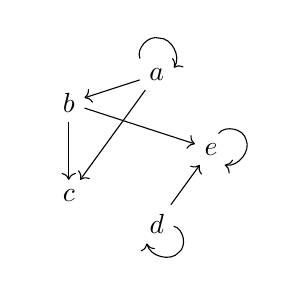
\begin{tikzpicture}
    %VARIABLES
    \pgfmathsetmacro{\gsize}{1}
    \pgfmathsetmacro{\gnum}{5}

    \foreach[count=\i] \element in {a,b,c,d,e} { %domain
        \node (\element) at (\i * 360 / \gnum:\gsize) {$\element$};
        \node (\element-) at (\i * 360 / \gnum:\gsize + 0.5) {};
      }
    \foreach \j/\l in {a/b, b/c, a/c, b/e, d/e} { %a to b
        \draw[->] (\j) -- (\l);
      }
    \foreach \j in {a,e,d} { %a to a
        \draw[->] (\j) to[bend left=65] (\j-)
        to[bend left=65] (\j);
      }
  \end{tikzpicture}
\end{center}
For Matrix Representation, this means that the matrix is anti-symmetric along the top left to bottom right diagonal:
\begin{center}
  $
    \bordermatrix{ & a & b & c & d \cr
      a & - & \bar{u} & \bar{v} & \bar{x} \cr
      b & u & - & \bar{w} & \bar{y} \cr
      c & v & w & - & \bar{z} \cr
      d & x & y & z & - \cr }
  $
  where
  \begin{tabular}{c}
    $u \in \{0,1\}$ \\
    $\vdots$        \\
    $z \in \{0,1\}$
  \end{tabular}
\end{center}

A binary relation of R on set $A$ is \textbf{Transitive} if for \textit{every} three elements $x,y,z \in A$,
if $x$R$y$ and $y$R$z$, then $x$R$z$. Logically, ($x$R$y \land y$R$z) \implies x$R$z$.
For Arrow Diagrams, this means the graph follows a hierarchy or kind of flow:
\begin{center}
  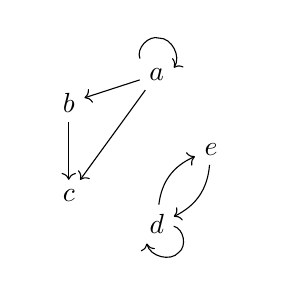
\begin{tikzpicture}
    %VARIABLES
    \pgfmathsetmacro{\gsize}{1}
    \pgfmathsetmacro{\gnum}{5}

    \foreach[count=\i] \element in {a,b,c,d,e} { %domain
        \node (\element) at (\i * 360 / \gnum:\gsize) {$\element$};
        \node (\element-) at (\i * 360 / \gnum:\gsize + 0.5) {};
      }
    \foreach \j/\l in {a/b,b/c,a/c} { %a to b
        \draw[->] (\j) -- (\l);
      }
    \foreach \j/\l in {d/e} { %a to b AND b to a
        \draw[->] (\j) to[bend left=20 / \gsize + 10] (\l);
        \draw[->] (\l) to[bend left=20 / \gsize + 10] (\j);
      }
    \foreach \j in {d,a} { %a to a
        \draw[->] (\j) to[bend left=65] (\j-)
        to[bend left=65] (\j);
      }
  \end{tikzpicture}
\end{center}
For Matrix Representation, it is much more difficult to determine transitivity, but here is an example:
\[
  \bordermatrix{ & a & b & c & d & e \cr
    a & 1 & 1 & 1 & 0 & 0 \cr
    b & 0 & 0 & 1 & 0 & 0 \cr
    c & 0 & 0 & 0 & 0 & 0 \cr
    d & 0 & 0 & 0 & 1 & 1 \cr
    e & 0 & 0 & 0 & 1 & 0 \cr }
\]

\subsection{Directed graphs, paths, and cycles}

A directed graph, or \textbf{Diagraph}, consists of a pair $(V,E)$, where $V$ is the set of vertices
and $E$ is the set of \textit{directed edges}. It is a subset of $V \times V$.
\begin{itemize}
  \item indegree: \# of edges pointing towards a vertex, $\text{indegree}(u) = \left\lvert\{v : (v,u) \in E\}\right\rvert$
  \item outdegree: \# of edges pointing away from a vertex, $\text{outdegree}(u) = \left\lvert\{u : (v,u) \in E\}\right\rvert$
\end{itemize}
A digraph is organized into a cartesian pair of the set of vertices and edge pairs:
\begin{align*}
  \text{Graph } G & = (V,E)                      \\
  V               & = \{a,b,c,d\}                \\
  E               & = \{(a,b),(b,c)(a,c),(d,d)\}
\end{align*}
\begin{center}
  \begin{tikzpicture}
    %VARIABLES
    \pgfmathsetmacro{\gsize}{1}
    \pgfmathsetmacro{\gnum}{4}

    \foreach[count=\i] \element in {a,b,c,d} { %domain
        \node (\element) at (\i * 360 / \gnum:\gsize) {$\element$};
        \node (\element-) at (\i * 360 / \gnum:\gsize + 0.5) {};
      }
    \foreach \j/\l in {a/b,b/c,a/c} { %a to b
        \draw[->] (\j) -- (\l);
      }
    \foreach \j/\l in {} { %a to b AND b to a
        \draw[->] (\j) to[bend left=20 / \gsize + 10] (\l);
        \draw[->] (\l) to[bend left=20 / \gsize + 10] (\j);
      }
    \foreach \j in {d} { %a to a
        \draw[->] (\j) to[bend left=65] (\j-)
        to[bend left=65] (\j);
      }
  \end{tikzpicture}
\end{center}
\begin{align*}
  \text{indegree}(c) & = 2 & \text{outdegree}(a) & = 2 & a & \text{ is the \underline{tail} of edge $(a,b)$} \\
  \text{indegree}(d) & = 1 & \text{outdegree}(d) & = 1 & b & \text{ is the \underline{head} of edge $(a,b)$} \\
\end{align*}

A digraph is mathematically the same as a relation. Here is an example of the internet as a graph:
\begin{align*}
  \text{Graph } G & = (V,E)                                                     \\
  V               & = \text{ set of all URLs}                                   \\
  E               & = \text{ set of all hyperlinks from one URL to another URL}
\end{align*}
\begin{align*}
  B   & = \text{ Blog}                   \\
  P   & = \text{ Pediatrician website}   \\
  PC  & = \text{ Pharmaceutical Company} \\
  AoP & = \text{ Academy of Pediatrics}
\end{align*}
\begin{center}
  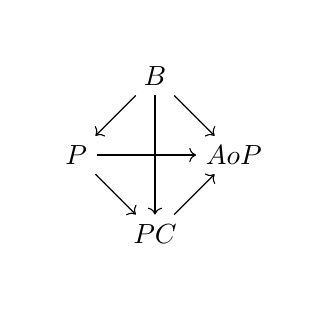
\begin{tikzpicture}
    %VARIABLES
    \pgfmathsetmacro{\gsize}{1}
    \pgfmathsetmacro{\gnum}{4}

    \foreach[count=\i] \element in {B, P, PC, AoP} { %domain
        \node (\element) at (\i * 360 / \gnum:\gsize) {$\element$};
        \node (\element-) at (\i * 360 / \gnum:\gsize + 0.5) {};
      }
    \foreach \j/\l in {B/P, B/PC, B/AoP, P/PC, P/AoP, PC/AoP} { %a to b
        \draw[->] (\j) -- (\l);
      }
    \foreach \j/\l in {} { %a to b AND b to a
        \draw[->] (\j) to[bend left=20 / \gsize + 10] (\l);
        \draw[->] (\l) to[bend left=20 / \gsize + 10] (\j);
      }
    \foreach \j in {} { %a to a
        \draw[->] (\j) to[bend left=65] (\j-)
        to[bend left=65] (\j);
      }
  \end{tikzpicture}
\end{center}

\subsubsection*{Walks in Directed Graphs}

A \textit{walk} is a sequence of vertices and edges. For example, a walk from $v_0$ to $v_l$ is notated as:
\[
  \left\langle v_0,(v_0,v_1), v_1,(v_1,v_2), \ldots,(v_{l-1},v_l), v_l\right\rangle
\]
where each edge in the sequence appears after its tail and before its head. A walk can also be a set of vertices:
\[
  \left\langle v_0, v_1, \ldots, v_l\right\rangle
\]
provided that the edges between the vertices \textit{actually exist}.
The \textbf{length} of a walk is the number of edges traversed.
\begin{itemize}
  \item \textbf{Open walk}: first and last vertices are \textit{not} the same
  \item \textbf{Closed walk}: first and last vertices \textit{are} the same.
\end{itemize}

\subsubsection*{Trails, Circuits, Paths, Cycles}
\begin{itemize}
  \item \textbf{Trail}: \textit{open} walk in which no edge occurs more than once.
  \item \textbf{Circuit}: \textit{closed} walk in which no edge occurs more than once. A circuit is a closed trail.
  \item \textbf{Path}: \textit{trail} where no vertex occurs more than once.
  \item \textbf{Cycle}: \textit{circuit} where no vertex occurs more than once, \textit{except} for the first and last, which are the same.
\end{itemize}
Here are some examples:
\begin{align*}
  \left\langle a,c,d,a\right\rangle   & \text{ is a \textbf{cycle}: only the first and last vertices are repeated.} \\
  \left\langle a,c,a,d,a\right\rangle & \text{ is a \textbf{circuit}: vertices are repeated, but not edges}         \\
  \left\langle a,b,c,b,d\right\rangle & \text{ is a \textbf{trail}: open, vertices are repeated, but not edges}
\end{align*}

\subsection{Composition of relations}

\begin{itemize}
  \item one-to-one correspondence between digraphs and binary relations
  \item arrow diagram for a binary relation \textit{is} a directed graph
\end{itemize}
The \textbf{composition} of relations R and S on set $A$ is denoted as S$\circ$R. Logically, this is what is means:
\[
  (a,c) \in S \circ R \iff \exists~ b : (b \in A \land (a,b) \in R \land (b,c) \in S)
\]
Composition is applied \textit{right to left}, much like composition of functions, or matrix transformations.
Therefore, S$\circ$R means R is applied first, then S.
\begin{center}
  \begin{tikzpicture}
    %VARIABLES
    \pgfmathsetmacro{\gsize}{1};
    \pgfmathsetmacro{\gnum}{4};


    \foreach[count=\i] \element in {a,b,c,d} { %domain
        \node (\element) at (\i * 360 / \gnum:\gsize) {$\element$};
        \node (\element-) at (\i * 360 / \gnum:\gsize + 0.5) {};
      }
    \foreach \j/\l in {a/d,b/c} { %a to b
        \draw[->] (\j) -- (\l);
      }
    \foreach \j/\l in {c/d} { %a to b AND b to a
        \draw[->] (\j) to[bend left=20 / \gsize + 10] (\l);
        \draw[->] (\l) to[bend left=20 / \gsize + 10] (\j);
      }
    \foreach \j in {b} { %a to a
        \draw[->] (\j) to[bend left=65] (\j-)
        to[bend left=65] (\j);
      }
    \node[anchor=east] (name) at (145:\gsize+.5) {R}; %relation name
  \end{tikzpicture}
  \qquad
  \begin{tikzpicture}
    %VARIABLES
    \pgfmathsetmacro{\gsize}{1};
    \pgfmathsetmacro{\gnum}{4};


    \foreach[count=\i] \element in {a,b,c,d} { %domain
        \node (\element) at (\i * 360 / \gnum:\gsize) {$\element$};
        \node (\element-) at (\i * 360 / \gnum:\gsize + 0.5) {};
      }
    \foreach \j/\l in {b/a,b/d,d/c} { %a to b
        \draw[->] (\j) -- (\l);
      }
    \foreach \j/\l in {} { %a to b AND b to a
        \draw[->] (\j) to[bend left=20 / \gsize + 10] (\l);
        \draw[->] (\l) to[bend left=20 / \gsize + 10] (\j);
      }
    \foreach \j in {} { %a to a
        \draw[->] (\j) to[bend left=65] (\j-)
        to[bend left=65] (\j);
      }
    \node[anchor=east] (name) at (145:\gsize+.5) {S}; %relation name
  \end{tikzpicture}
  \qquad
  \begin{tikzpicture}
    %VARIABLES
    \pgfmathsetmacro{\gsize}{1};
    \pgfmathsetmacro{\gnum}{4};


    \foreach[count=\i] \element in {a,b,c,d} { %domain
        \node (\element) at (\i * 360 / \gnum:\gsize) {$\element$};
        \node (\element-) at (\i * 360 / \gnum:\gsize + 0.5) {};
      }
    \foreach \j/\l in {a/c,b/a,b/d} { %a to b
        \draw[->] (\j) -- (\l);
      }
    \foreach \j/\l in {} { %a to b AND b to a
        \draw[->] (\j) to[bend left=20 / \gsize + 10] (\l);
        \draw[->] (\l) to[bend left=20 / \gsize + 10] (\j);
      }
    \foreach \j in {c} { %a to a
        \draw[->] (\j) to[bend left=65] (\j-)
        to[bend left=65] (\j);
      }
    \node[anchor=east] (name) at (145:\gsize+.5) {S$\circ$R}; %relation name
  \end{tikzpicture}
\end{center}

\subsection{Graph powers and the transitive closure}

A relation can be composed with itself. For example, consider relation P, which expresses parent-child relationship.
\begin{center}
  \begin{tabular}{l}
    $x$P$y$ means $x$ is the parent of $y$. \\
    $x$P$\circ$P$z$ means $x$ is the grandparent of $z$
  \end{tabular}
\end{center}
A relation composed with itself also represents walks of different lengths.
\begin{center}
  \begin{tabular}{l}
    P$\circ$P represents all walks of length 2. \\
    P$\circ$P$\circ$P represents all walks of length 3.
  \end{tabular}
\end{center}

\subsubsection*{The Graph Power Theorem}:
Let G be a directed graph. Let $u$ and $v$ be any two vertices in G. There is an edge from $u$ to $v$ in $G^k$
if and only if there is a walk of length $k$ from $u$ to $v$ in G.
\begin{align*}
  R^1 & = R                                         \\
  R^k & = R \circ R^{k-1} \text{ for all } k \geq 2
\end{align*}

\subsubsection*{Transitive Closure}
\[
  G^+ = G^1 \cup G^2 \cup G^3 \cup \cdots
\]
if $G$ is not infinite, only up to the number of vertices are required for a complete graph of $G^+$
\[
  G^+ = G^1 \cup G^2 \cup G^3 \cup \cdots \cup G^{\left\lvert V\right\rvert}
\]
Here is an example of a series of graph powers:
\begin{center}
  \begin{tikzpicture}
    %VARIABLES
    \pgfmathsetmacro{\gsize}{1};
    \pgfmathsetmacro{\gnum}{4};

    \foreach[count=\i] \element in {a,b,c,d} { %domain
        \node (\element) at (\i * 360 / \gnum:\gsize) {$\element$};
        \node (\element-) at (\i * 360 / \gnum:\gsize + 0.5) {};
      }
    \foreach \j/\l in {b/a,c/b,c/d} { %a to b
        \draw[->] (\j) -- (\l);
      }
    \foreach \j/\l in {a/d} { %a to b AND b to a
        \draw[->] (\j) to[bend left=20 / \gsize + 10] (\l);
        \draw[->] (\l) to[bend left=20 / \gsize + 10] (\j);
      }
    \foreach \j in {} { %a to a
        \draw[->] (\j) to[bend left=65] (\j-)
        to[bend left=65] (\j);
      }
    \node[anchor=east] (name) at (145:\gsize+.5) {$G$}; %relation name
  \end{tikzpicture}
  \quad
  \begin{tikzpicture}
    %VARIABLES
    \pgfmathsetmacro{\gsize}{1};
    \pgfmathsetmacro{\gnum}{4};

    \foreach[count=\i] \element in {a,b,c,d} { %domain
        \node (\element) at (\i * 360 / \gnum:\gsize) {$\element$};
        \node (\element-) at (\i * 360 / \gnum:\gsize + 0.5) {};
      }
    \foreach \j/\l in {b/d,c/a} { %a to b
        \draw[->] (\j) -- (\l);
      }
    \foreach \j/\l in {} { %a to b AND b to a
        \draw[->] (\j) to[bend left=20 / \gsize + 10] (\l);
        \draw[->] (\l) to[bend left=20 / \gsize + 10] (\j);
      }
    \foreach \j in {a,d} { %a to a
        \draw[->] (\j) to[bend left=65] (\j-)
        to[bend left=65] (\j);
      }
    \node[anchor=east] (name) at (145:\gsize+.5) {$G^2$}; %relation name
  \end{tikzpicture}
  \quad
  \begin{tikzpicture}
    %VARIABLES
    \pgfmathsetmacro{\gsize}{1};
    \pgfmathsetmacro{\gnum}{4};

    \foreach[count=\i] \element in {a,b,c,d} { %domain
        \node (\element) at (\i * 360 / \gnum:\gsize) {$\element$};
        \node (\element-) at (\i * 360 / \gnum:\gsize + 0.5) {};
      }
    \foreach \j/\l in {b/a,c/d} { %a to b
        \draw[->] (\j) -- (\l);
      }
    \foreach \j/\l in {a/d} { %a to b AND b to a
        \draw[->] (\j) to[bend left=20 / \gsize + 10] (\l);
        \draw[->] (\l) to[bend left=20 / \gsize + 10] (\j);
      }
    \foreach \j in {} { %a to a
        \draw[->] (\j) to[bend left=65] (\j-)
        to[bend left=65] (\j);
      }
    \node[anchor=east] (name) at (145:\gsize+.5) {$G^3$}; %relation name
  \end{tikzpicture}
  \quad
  \begin{tikzpicture}
    %VARIABLES
    \pgfmathsetmacro{\gsize}{1};
    \pgfmathsetmacro{\gnum}{4};

    \foreach[count=\i] \element in {a,b,c,d} { %domain
        \node (\element) at (\i * 360 / \gnum:\gsize) {$\element$};
        \node (\element-) at (\i * 360 / \gnum:\gsize + 0.5) {};
      }
    \foreach \j/\l in {c/a,b/d} { %a to b
        \draw[->] (\j) -- (\l);
      }
    \foreach \j/\l in {} { %a to b AND b to a
        \draw[->] (\j) to[bend left=20 / \gsize + 10] (\l);
        \draw[->] (\l) to[bend left=20 / \gsize + 10] (\j);
      }
    \foreach \j in {a,d} { %a to a
        \draw[->] (\j) to[bend left=65] (\j-)
        to[bend left=65] (\j);
      }
    \node[anchor=east] (name) at (145:\gsize+.5) {$G^4$}; %relation name
  \end{tikzpicture}
\end{center}
\begin{center}
  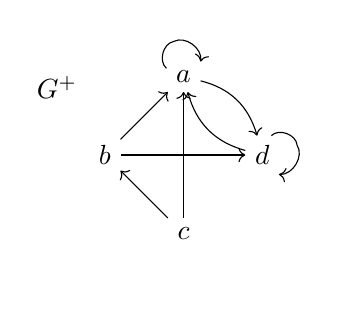
\begin{tikzpicture}
    %VARIABLES
    \pgfmathsetmacro{\gsize}{1};
    \pgfmathsetmacro{\gnum}{4};

    \foreach[count=\i] \element in {a,b,c,d} { %domain
        \node (\element) at (\i * 360 / \gnum:\gsize) {$\element$};
        \node (\element-) at (\i * 360 / \gnum:\gsize + 0.5) {};
      }
    \foreach \j/\l in {b/a, b/d, c/b, c/a} { %a to b
        \draw[->] (\j) -- (\l);
      }
    \foreach \j/\l in {a/d} { %a to b AND b to a
        \draw[->] (\j) to[bend left=20 / \gsize + 10] (\l);
        \draw[->] (\l) to[bend left=20 / \gsize + 10] (\j);
      }
    \foreach \j in {a,d} { %a to a
        \draw[->] (\j) to[bend left=65] (\j-)
        to[bend left=65] (\j);
      }
    \node[anchor=east] (name) at (145:\gsize+.5) {$G^+$}; %relation name
  \end{tikzpicture}
\end{center}

\subsubsection*{Finding the Transitive Closure of a Relation $R$ on set $A$}
Repeat until no pair is added to $R$.
\begin{center}
  If there are 3 elements $x,y,z \in A$ such that $x$R$y$ and $y$R$z$ but not $x$R$z$, add $x$R$z$ to R.
\end{center}
For example:
\begin{center}
  \begin{tikzpicture}
    %VARIABLES
    \pgfmathsetmacro{\gsize}{1.5};
    \pgfmathsetmacro{\gnum}{5};

    \foreach[count=\i] \element in {a,b,c,d,e} { %domain
        \node (\element) at (\i * 360 / \gnum:\gsize) {$\element$};
        \node (\element-) at (\i * 360 / \gnum:\gsize + 0.5) {};
      }
    \foreach \j/\l in {a/b, b/e, d/e} { %a to b
        \draw[->] (\j) -- (\l);
      }
    \foreach \j/\l in {b/c} { %a to b AND b to a
        \draw[->] (\j) to[bend left=20 / \gsize + 10] (\l);
        \draw[->] (\l) to[bend left=20 / \gsize + 10] (\j);
      }
    \foreach \j in {b,e} { %a to a
        \draw[->] (\j) to[bend left=65] (\j-)
        to[bend left=65] (\j);
      }
    \node[anchor=east] (name) at (145:\gsize+.5) {Relation}; %relation name
  \end{tikzpicture}
  \quad
  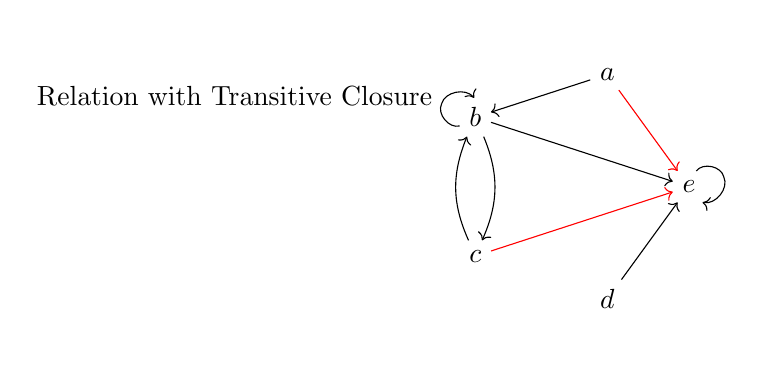
\begin{tikzpicture}
    %VARIABLES
    \pgfmathsetmacro{\gsize}{1.5};
    \pgfmathsetmacro{\gnum}{5};

    \foreach[count=\i] \element in {a,b,c,d,e} { %domain
        \node (\element) at (\i * 360 / \gnum:\gsize) {$\element$};
        \node (\element-) at (\i * 360 / \gnum:\gsize + 0.5) {};
      }
    \foreach \j/\l in {a/b, b/e, d/e} { %a to b
        \draw[->] (\j) -- (\l);
      }
    \foreach \j/\l in {b/c} { %a to b AND b to a
        \draw[->] (\j) to[bend left=20 / \gsize + 10] (\l);
        \draw[->] (\l) to[bend left=20 / \gsize + 10] (\j);
      }
    \foreach \j in {b,e} { %a to a
        \draw[->] (\j) to[bend left=65] (\j-)
        to[bend left=65] (\j);
      }
    \foreach \j/\l in {a/e,c/e} { %a to b in red
        \draw[->, red] (\j) -- (\l);
      }
    \node[anchor=east] (name) at (145:\gsize+.5) {Relation with Transitive Closure}; %relation name
  \end{tikzpicture}
\end{center}
\begin{center}
  Edges added to find transitive closure are shown in red.
\end{center}

\subsection{Matrix multiplication and graph powers}
An $n \times m$ \textbf{matrix} over set $S$ is an array of elements from $S$ with $n$ rows and $m$ columns.
Each element in a matrix is called an \textit{entry}.
A \textbf{square matrix} has the same number of rows and columns.
Here are a number of example matrixes
\begin{align*}
  \begin{bmatrix}
    1  & 3  \\
    3  & -5 \\
    -2 & -2
  \end{bmatrix}
                                             &  &
  \begin{bmatrix}
    1.1  & 3.0  & -5.4 \\
    -2.2 & -2.1 & 1
  \end{bmatrix}
                                             &  &
  \begin{bmatrix}
    1 & 0 \\
    1 & 1
  \end{bmatrix}                                                                                                                          \\
  3 \times 2 \text{ matrix over } \mathbb{Z} &  & 2 \times 3 \text{ matrix over } \mathbb{Z} &  & 2 \times 2 \text{ matrix over } \{0,1\}
\end{align*}
A directed graph $G$ can be represented by a Matrix.
\begin{center}
  $n$ vertices $\rightarrow$ $n \times n$ matrix over the set \{0,1\}, called an \textbf{adjacency matrix}
\end{center}
\begin{center}
  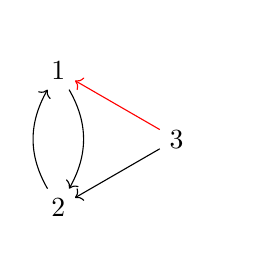
\begin{tikzpicture}
    %VARIABLES
    \pgfmathsetmacro{\gsize}{1};
    \pgfmathsetmacro{\gnum}{3};

    \foreach[count=\i] \element in {1,2,3} { %domain
        \node (\element) at (\i * 360 / \gnum:\gsize) {$\element$};
        \node (\element-) at (\i * 360 / \gnum:\gsize + 0.5) {};
      }
    \foreach \j/\l in {3/2} { %a to b
        \draw[->] (\j) -- (\l);
      }
    \foreach \j/\l in {1/2} { %a to b AND b to a
        \draw[->] (\j) to[bend left=20 / \gsize + 10] (\l);
        \draw[->] (\l) to[bend left=20 / \gsize + 10] (\j);
      }
    \foreach \j in {} { %a to a
        \draw[->] (\j) to[bend left=65] (\j-)
        to[bend left=65] (\j);
      }
    \foreach \j/\l in {3/1} { %a to b in red
        \draw[->, red] (\j) -- (\l);
      }
  \end{tikzpicture}
  $
    \begin{bmatrix}
      0                       & 1 & 0 \\
      1                       & 0 & 0 \\
      \text{\textcolor{red}1} & 1 & 0
    \end{bmatrix}
  $
\end{center}
A \textbf{boolean matrix} is a matrix over the set \{0,1\}, and boolean addition and multiplication are used.
The \textbf{dot product} of a matrix $A$ and $B$ is defined only if \# of columns in $A$ = \# of rows in $B$
\[
  A =
  \begin{bmatrix}
    1                       & 1                       & 1                       \\
    \text{\textcolor{red}1} & \text{\textcolor{red}0} & \text{\textcolor{red}1} \\
    0                       & 1                       & 0
  \end{bmatrix}
  \qquad
  B =
  \begin{bmatrix}
    1 & 0 & \text{\textcolor{green}1} \\
    0 & 0 & \text{\textcolor{green}1} \\
    1 & 0 & \text{\textcolor{green}1}
  \end{bmatrix}
\]
\begin{center}
  \begin{tabular}{cccccc}
    {\textcolor{red}1}            &   & {\textcolor{red}0}           &   & {\textcolor{red}1}                                         \\
    $\times$ {\textcolor{green}1} &   & $\times${\textcolor{green}1} &   & $\times$ {\textcolor{green}1}                              \\
    \hhline{-~-~-}
    1                             & + & 0                            & + & 1                             & = 1 = $(A \times B)_{2,3}$
  \end{tabular}
\end{center}

\subsubsection*{Matrix Product}
\begin{itemize}
  \item denoted as $AB$ or $A \cdot B$
  \item uses a series of dot products to compute
\end{itemize}
There are a number of properties of matrix multiplication:
\begin{center}
  \begin{tabular}{rc}
    \sout{Commutative} & $AB \not = BA$                                   \\
    Associative        & $(AB)C = A(BC)$                                  \\
    Distributive       & $A(B + C) = AB + AC$                             \\
                       & $(B+C)A = BA + CA$                               \\
    Multiplicative     & $IA = A$ and $AI = A$                            \\
                       & $OA = A$ and $AO = O$                            \\
    Dimension          & $(m \times n) \cdot (n \times k) = (m \times k)$
  \end{tabular}
\end{center}
$k^{th}$ power of a matrix:
\[
  A^k = \underbrace{A \cdot A \cdots A}_{k \text{ times}}
\]

If $G$ is a digraph, $G^k$ represents all walks of length $k$ in $G$.
There is an edge from vertex $v$ to vertex $w$ in $G^k$ if and only if there is a walk of length \textit{exactly}
$k$ from $v$ to $w$ in $G$. Matrix multiplication provides a systematic way of computing $G^k$.
\begin{enumerate}
  \item Take \textit{adjacency matrix} $A$ for graph $G$
  \item Compute $A^k$ by repeated \textit{matrix multiplication}
  \item Matrix $A^k$ is the \textit{adjacency matrix} for graph $G^k$.
\end{enumerate}

\subsubsection*{Relationship between powers of a graph and the powers of its adjacency matrix}
Let $G$ be a directed graph with $n$ vertices and let $A$ be the adjacency matrix for $G$.
Then for $k \geq 1$, $A^k$ is the adjacency matrix of $G^k$,
where boolean addition and multiplication are used to compute $A^k$.
\begin{center}
  Example:
  \qquad
  \begin{tikzpicture}
    %VARIABLES
    \pgfmathsetmacro{\gsize}{1};
    \pgfmathsetmacro{\gnum}{5};


    \foreach[count=\i] \element in {a,b,c,d,e} { %domain
        \node (\element) at (\i * 360 / \gnum:\gsize) {$\element$};
        \node (\element-) at (\i * 360 / \gnum:\gsize + 0.5) {};
      }
    \foreach \j/\l in {a/b,a/d,b/e} { %a to b
        \draw[->] (\j) -- (\l);
      }
    \foreach \j/\l in {d/e} { %a to b AND b to a
        \draw[->] (\j) to[bend left=20 / \gsize + 10] (\l);
        \draw[->] (\l) to[bend left=20 / \gsize + 10] (\j);
      }
    \foreach \j in {c} { %a to a
        \draw[->] (\j) to[bend left=65] (\j-)
        to[bend left=65] (\j);
      }
    \node[anchor=east] (name) at (145:\gsize+.5) {G}; %relation name
  \end{tikzpicture}
  \qquad
  \begin{tikzpicture}
    %VARIABLES
    \pgfmathsetmacro{\gsize}{1};
    \pgfmathsetmacro{\gnum}{5};

    \foreach[count=\i] \element in {a,b,c,d,e} { %domain
        \node (\element) at (\i * 360 / \gnum:\gsize) {$\element$};
        \node (\element-) at (\i * 360 / \gnum:\gsize + 0.5) {};
      }
    \foreach \j/\l in {a/e,b/d} { %a to b
        \draw[->] (\j) -- (\l);
      }
    \foreach \j/\l in {} { %a to b AND b to a
        \draw[->] (\j) to[bend left=20 / \gsize + 10] (\l);
        \draw[->] (\l) to[bend left=20 / \gsize + 10] (\j);
      }
    \foreach \j in {c,d,e} { %a to a
        \draw[->] (\j) to[bend left=65] (\j-)
        to[bend left=65] (\j);
      }
    \node[anchor=east] (name) at (145:\gsize+.5) {G$^2$}; %relation name
  \end{tikzpicture}
  \qquad
  \begin{tikzpicture}
    %VARIABLES
    \pgfmathsetmacro{\gsize}{1};
    \pgfmathsetmacro{\gnum}{5};

    \foreach[count=\i] \element in {a,b,c,d,e} { %domain
        \node (\element) at (\i * 360 / \gnum:\gsize) {$\element$};
        \node (\element-) at (\i * 360 / \gnum:\gsize + 0.5) {};
      }
    \foreach \j/\l in {a/d,b/e} { %a to b
        \draw[->] (\j) -- (\l);
      }
    \foreach \j/\l in {e/d} { %a to b AND b to a
        \draw[->] (\j) to[bend left=20 / \gsize + 10] (\l);
        \draw[->] (\l) to[bend left=20 / \gsize + 10] (\j);
      }
    \foreach \j in {c} { %a to a
        \draw[->] (\j) to[bend left=65] (\j-)
        to[bend left=65] (\j);
      }
    \node[anchor=east] (name) at (145:\gsize+.5) {G$^3$}; %relation name
  \end{tikzpicture}
\end{center}
\[
  A =
  \begin{bmatrix}
    0 & 1 & 0 & 1 & 0 \\
    0 & 0 & 0 & 0 & 1 \\
    0 & 0 & 1 & 0 & 0 \\
    0 & 0 & 0 & 0 & 1 \\
    0 & 0 & 0 & 1 & 0
  \end{bmatrix}
  \quad
  A^2 =
  \begin{bmatrix}
    0 & 0 & 0 & 0 & 1 \\
    0 & 0 & 0 & 1 & 0 \\
    0 & 0 & 1 & 0 & 0 \\
    0 & 0 & 0 & 1 & 0 \\
    0 & 0 & 0 & 0 & 1
  \end{bmatrix}
  \quad
  A^3 =
  \begin{bmatrix}
    0 & 0 & 0 & 0 & 0 \\
    0 & 0 & 0 & 0 & 1 \\
    0 & 0 & 1 & 0 & 0 \\
    0 & 0 & 0 & 0 & 1 \\
    0 & 0 & 0 & 1 & 0
  \end{bmatrix}
\]

\subsubsection*{Matrix Sum}
\begin{itemize}
  \item denoted as $A + B$
  \item well-defined if same \# of row and \# of columns
\end{itemize}
\[
  (A+B)_{i,j} = A_{i,j} + B_{i,j} \text{ for all $i$ and $j$ in range of $A$ or $B$}
\]
For example,
\begin{center}
  \begin{tabular}{ccccc}
    \text{\textcolor{blue}0} & + & \text{\textcolor{red}1} & = & \text{\textcolor{purple}1} \\
    $
      \begin{bmatrix}
        1                        & 0 & 1 \\
        \text{\textcolor{blue}0} & 1 & 0 \\
        0                        & 0 & 1
      \end{bmatrix}
    $                        & + &
    $
      \begin{bmatrix}
        0                       & 0 & 1 \\
        \text{\textcolor{red}1} & 1 & 0 \\
        0                       & 1 & 1
      \end{bmatrix}
    $                        & = &
    $
      \begin{bmatrix}
        1                          & 0 & 1 \\
        \text{\textcolor{purple}1} & 1 & 0 \\
        0                          & 1 & 1
      \end{bmatrix}
    $                                                                                       \\
    $A$                      & + & $B$                     & = & $A+B$
  \end{tabular}
\end{center}

\subsubsection*{Addition and Graph Union}
Let $G$ and $H$ be two directed graphs with the same vertex set.
Let $A$ be adjacency matrix for $G$ and $B$ the adjacency matrix for $H$.

Then the adjacency matrix for $G \cup H = A + B$, where boolean addition is used on the entries of matrices $A$ and $B$.
\begin{center}
  \begin{tabular}{ccccc}
    \begin{tikzpicture}
      %VARIABLES
      \pgfmathsetmacro{\gsize}{1};
      \pgfmathsetmacro{\gnum}{4};

      \foreach[count=\i] \element in {1,2,3,4} { %domain
          \node (\element) at (\i * 360 / \gnum:\gsize) {$\element$};
          \node (\element-) at (\i * 360 / \gnum:\gsize + 0.5) {};
        }
      \foreach \j/\l in {2/4,3/2} { %a to b
          \draw[->] (\j) -- (\l);
        }
      \foreach \j/\l in {1/2} { %a to b AND b to a
          \draw[->] (\j) to[bend left=20 / \gsize + 10] (\l);
          \draw[->] (\l) to[bend left=20 / \gsize + 10] (\j);
        }
      \foreach \j in {4} { %a to a
          \draw[->] (\j) to[bend left=65] (\j-)
          to[bend left=65] (\j);
        }
    \end{tikzpicture} & $\cup$ &
    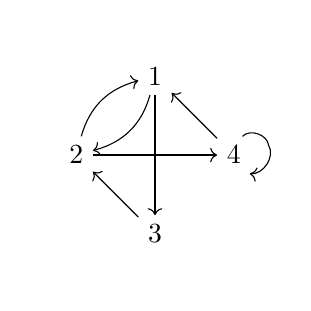
\begin{tikzpicture}
      %VARIABLES
      \pgfmathsetmacro{\gsize}{1};
      \pgfmathsetmacro{\gnum}{4};

      \foreach[count=\i] \element in {1,2,3,4} { %domain
          \node (\element) at (\i * 360 / \gnum:\gsize) {$\element$};
          \node (\element-) at (\i * 360 / \gnum:\gsize + 0.5) {};
        }
      \foreach \j/\l in {1/3,2/4,3/2,4/1} { %a to b
          \draw[->] (\j) -- (\l);
        }
      \foreach \j/\l in {1/2} { %a to b AND b to a
          \draw[->] (\j) to[bend left=20 / \gsize + 10] (\l);
          \draw[->] (\l) to[bend left=20 / \gsize + 10] (\j);
        }
      \foreach \j in {4} { %a to a
          \draw[->] (\j) to[bend left=65] (\j-)
          to[bend left=65] (\j);
        }
    \end{tikzpicture} & =      &
    \begin{tikzpicture}
      %VARIABLES
      \pgfmathsetmacro{\gsize}{1};
      \pgfmathsetmacro{\gnum}{4};

      \foreach[count=\i] \element in {1,2,3,4} { %domain
          \node (\element) at (\i * 360 / \gnum:\gsize) {$\element$};
          \node (\element-) at (\i * 360 / \gnum:\gsize + 0.5) {};
        }
      \foreach \j/\l in {4/1,3/2,1/3} { %a to b
          \draw[->] (\j) -- (\l);
        }
      \foreach \j/\l in {1/2} { %a to b AND b to a
          \draw[->] (\j) to[bend left=20 / \gsize + 10] (\l);
          \draw[->] (\l) to[bend left=20 / \gsize + 10] (\j);
        }
      \foreach \j in {4} { %a to a
          \draw[->] (\j) to[bend left=65] (\j-)
          to[bend left=65] (\j);
        }
    \end{tikzpicture}                                  \\
    $G$                                                                           & $\cup$ & $H$ & = & $G \cup H$ \\
    $A$                                                                           & +      & $B$ & = & $A+B$      \\
    $
      \begin{bmatrix}
        0 & 1 & 0 & 0 \\
        1 & 0 & 0 & 1 \\
        0 & 1 & 0 & 0 \\
        0 & 0 & 0 & 1 \\
      \end{bmatrix}
    $                                                                             & +      &
    $
      \begin{bmatrix}
        0 & 1 & 1 & 0 \\
        0 & 0 & 0 & 1 \\
        0 & 1 & 0 & 0 \\
        1 & 0 & 0 & 0 \\
      \end{bmatrix}
    $                                                                             & =      &
    $
      \begin{bmatrix}
        0 & 1 & 1 & 0 \\
        1 & 0 & 0 & 1 \\
        0 & 1 & 0 & 0 \\
        1 & 0 & 0 & 1 \\
      \end{bmatrix}
    $
  \end{tabular}
\end{center}
For digraph $G$ and adjacency matrix $A$ for $G$:
\begin{align*}
  G^+ & = G^1 \cup G^2 \cup G^3 \cup \cdots \cup G^n \\
  A^+ & = A^1 + A^2 + A^3 + \cdots + A^n
\end{align*}

\subsubsection*{Condition for well-defined matrix multiplication}
$A_{m \times n} \times B_{s \times t}$ is only defined when $n = s$, and $A \times B$ has dimensions $m \times t$.
For example:
\[
  A_{3 \times 3}
  \begin{bmatrix}
    0 & 2 & 3 \\
    1 & 0 & 1 \\
    2 & 0 & 1
  \end{bmatrix}
  \times
  B_{3 \times 1}
  \begin{bmatrix}
    1 \\
    2 \\
    0
  \end{bmatrix}
  =
  (A \times B)_{3 \times 1}
  \begin{bmatrix}
    5 \\
    4 \\
    0
  \end{bmatrix}
\]

\subsection{Partial orders}

A relation on set $A$ is a \textbf{partial order} if it is:
\begin{itemize}
  \item reflexive
  \item transitive
  \item anti-symmetric
\end{itemize}
Notation:\quad $a \preceq b$ used to express $a$R$b$

Domain along with a partial order defined on it is denoted $(A, \preceq)$
and is called a \textbf{partial ordered set} or \textbf{poset}.
\[
  \preceq \not = \leq \text{ (notice the curves)}
\]
Two elements of a poset are said to be \textit{comparable} if $x \preceq y$ or $x \succeq y$.
Otherwise they are said to be \textit{incomparable}.
A partial order is a \textit{total order} if \underline{every} two elements in the domain are \textit{comparable}.

Here is an example of a partial order:
\begin{center}
  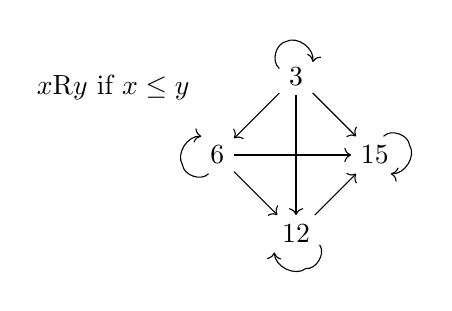
\begin{tikzpicture}
    %VARIABLES
    \pgfmathsetmacro{\gsize}{1};
    \pgfmathsetmacro{\gnum}{4};

    \foreach[count=\i] \element in {3,6,12,15} { %domain
        \node (\element) at (\i * 360 / \gnum:\gsize) {$\element$};
        \node (\element-) at (\i * 360 / \gnum:\gsize + 0.5) {};
      }
    \foreach \j/\l in {3/6,3/12,3/15,6/12,6/15,12/15} { %a to b
        \draw[->] (\j) -- (\l);
      }
    \foreach \j in {3,6,12,15} { %a to a
        \draw[->] (\j) to[bend left=65] (\j-)
        to[bend left=65] (\j);
      }
    \node[anchor=east] (name) at (145:\gsize+.5) {$x$R$y$ if $x \leq y$}; %relation name
  \end{tikzpicture}
\end{center}
\begin{itemize}
  \item An element $x$ is \textbf{minimal} element if there is no such $y \not = x$ such that $y \preceq x$
  \item An element $x$ is \textbf{maximal} element if there is no such $y \not = x$ such that $x \preceq y$
\end{itemize}

\subsubsection*{Hasse Diagram}
\begin{itemize}
  \item useful way to depict a partial order on a finite set
  \item each element is represented by a point
  \item shows relationships by placing elements that are greater than others toward the top of the diagram.
\end{itemize}
\textbf{Rules for placement and for connecting segments}
\begin{itemize}
  \item if $x \preceq y$, then make $x$ appear lower in the diagram than $y$
  \item if $x \preceq y$, and there is no such $z$ that $x \preceq z \preceq y$, then draw a segment connecting $x$ and $y$
\end{itemize}
Examples: Hasse Diagrams for a partial order on the power set of $\{1,2,3\}$, and $\{1,2,3,4,5,6\}$.
\begin{center}
  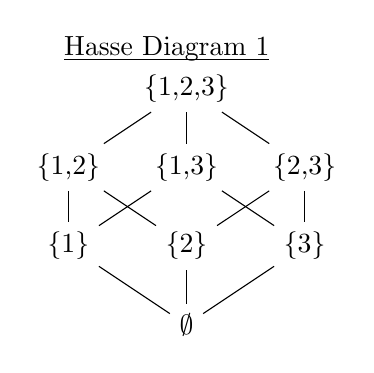
\begin{tikzpicture}
    %VARIABLES
    \pgfmathsetmacro{\spacing}{1.5};

    \foreach \rank/\elements/\size in {
    1/{{\{1,2,3\}}}/1, 2/{{\{1,2\}},{\{1,3\}},{\{2,3\}}}/3, 3/{{\{1\}},{\{2\}},{\{3\}}}/3, 4/{$\emptyset$}/1
    } {
    \foreach[count = \i] \element in \elements {
      \node (\rank-\i) at (\i * \spacing - \size / 2 * \spacing, -\rank) {\element};
    }
    }
    \foreach \j/\ls in {1-1/{2-1,2-2,2-3},2-1/{3-1,3-2},2-2/{3-1,3-3},2-3/{3-2,3-3},4-1/{3-1,3-2,3-3}} {\foreach \l in \ls {\draw (\j) -- (\l);}}
    \node (name) at (0.5,-0.5) {\underbar{Hasse Diagram 1}}; %name
  \end{tikzpicture}
  \qquad
  \begin{tikzpicture}
    %VARIABLES
    \pgfmathsetmacro{\spacing}{1.5};
    \foreach \rank/\elements/\size in {1/{6}/1, 2/{5}/1, 3/{4}/1, 4/{3}/1, 5/{2}/1, 6/{1}/1} {
    \foreach[count = \i] \element in \elements {
      \node (\rank-\i) at (\i * \spacing - \size / 2 * \spacing, -\rank) {\element};
    }
    }
    \foreach \j/\ls in {1-1/{2-1},2-1/{3-1},3-1/{4-1},4-1/{5-1},5-1/{6-1}} {\foreach \l in \ls {\draw (\j) -- (\l);}}
    \node (name) at (0.5,-0.5) {\underbar{Hasse Diagram 2}}; %name
  \end{tikzpicture}
\end{center}
The first example uses a rule of $A \preceq B \leftrightarrow A \subseteq B$,
while the second example uses a rule of $x \preceq y \leftrightarrow x \leq y$.

In general, if two elements are incomparable, then they are not connected \underline{at all} by a path of line segments
or the only paths between $x$ and $y$ require a change in direction from up to down or down to up.
Consider this partial order on the set $\{A,B,C,D,E,F,G\}$:
\begin{center}
  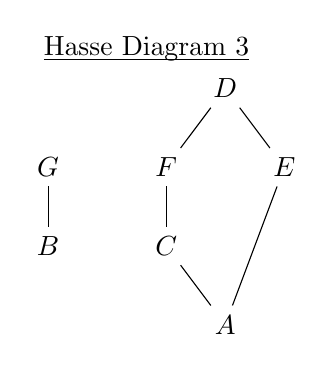
\begin{tikzpicture}
    %VARIABLES
    \pgfmathsetmacro{\spacing}{1.5};
    \foreach \rank/\elements/\size in {1/{ ,D}/2, 2/{G,F,E}/3, 3/{B,C}/3, 4/{ ,A}/2} {
    \foreach[count = \i] \element in \elements {
      \node (\element) at (\i * \spacing - \size / 2 * \spacing, -\rank) {$\element$};
    }
    }
    \foreach \j/\ls in {G/{B},D/{F,E},C/{F,A},E/{A}} {\foreach \l in \ls {\draw (\j) -- (\l);}}
    \node (name) at (0.5,-0.5) {\underbar{Hasse Diagram 3}}; %name
  \end{tikzpicture}
\end{center}
In this example, $B \preceq G$, and $A \preceq D$, but $B$ and $F$ are \underline{not} comparable.

\subsection{Strict orders and directed acyclic graphs}

\begin{itemize}
  \item Partial Order acts $\preceq$ on a domain
  \item Strict Order acts $\prec$ on a domain
\end{itemize}
A relation $R$ is a \textbf{Strict Order} if $R$ is \textit{transitive, anti-symmetric,} and \textit{anti-reflexive}.
\begin{itemize}
  \item two elements are comparable if $x \prec y$ or $x \succ y$, and otherwise incomparable
  \item strict order is a \textit{total order} if \underline{every} pair of elements is comparable
  \item element $x$ is \textbf{minimal} if no $y$ exists such that $y \prec x$
  \item element $x$ is \textbf{maximal} if no $y$ exists such that $x \prec y$
\end{itemize}
Here is an example of a strict order:
\begin{center}
  \begin{tikzpicture}
    %VARIABLES
    \pgfmathsetmacro{\gsize}{2};
    \pgfmathsetmacro{\gnum}{6};

    \foreach[count=\i] \element in {c,b,a,d,f,e} { %domain
        \node (\element) at (\i * 360 / \gnum:\gsize) {$\element$};
        \node (\element-) at (\i * 360 / \gnum:\gsize + 0.5) {};
      }
    \foreach \j/\ls in {a/{b,c,e},d/{f},b/{e},c/{e}} {\foreach \l in \ls {\draw[->] (\j) -- (\l);}}
  \end{tikzpicture}
  \qquad
  \begin{tabular}{rl}
    maximal: & $e$ and $f$ \\
    minimal: & $a$ and $d$
  \end{tabular}
\end{center}
Strict orders are also anti-symmetric. Consider a relation R that is transitive and anti-reflexive.
Then R is also anti-symmetric.

\subsubsection*{Directed Acyclic Graphs, DAGs}
A directed acyclic graph is a directed graph that has no cycles. For example, consider this DAG:
\begin{center}
  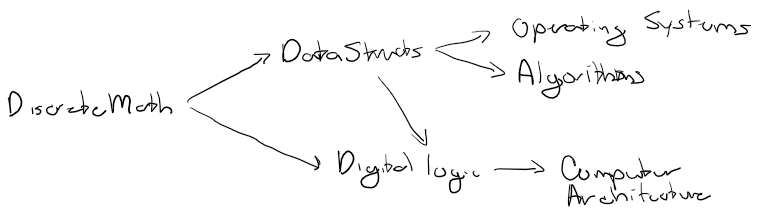
\includegraphics[width=.6\linewidth]{resources/dag prereq.png}
\end{center}
\textbf{Theorem: Directed Acyclic Graphs and Strict Orders}
Let $G$ be a directed graph. $G$ has no cycles if and only if $G^+$ is a strict order.
\begin{center}
  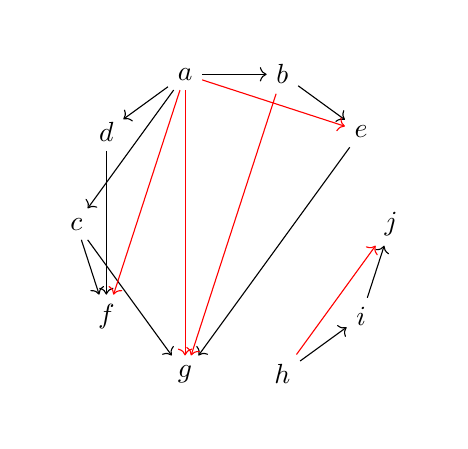
\begin{tikzpicture}
    %VARIABLES
    \pgfmathsetmacro{\gsize}{2};
    \pgfmathsetmacro{\gnum}{10};

    \foreach[count=\i] \element in {e,b,a,d,c,f,g,h,i,j} { %domain
        \node (\element) at (\i * 360 / \gnum:\gsize) {$\element$};
        \node (\element-) at (\i * 360 / \gnum:\gsize + 0.5) {};
      }
    \foreach \j/\ls in {a/{b,c,d},b/{e},c/{g,f},d/{f},e/{g},h/{i},i/{j}} {\foreach \l in \ls {\draw[->] (\j) -- (\l);}}
    \foreach \j/\ls in {a/{e,f,g},b/{g},h/{j}} {\foreach \l in \ls {\draw[->, red] (\j) -- (\l);}}
  \end{tikzpicture}
  \qquad
  \begin{tabular}{c}
    $G$ is a DAG                          \\
    Edges added by $G^+$ are shown in red \\
    Minimal: $a$ and $h$                  \\
    Maximal: $g$, $f$, and $j$
  \end{tabular}
\end{center}
Consider another example of precedence constraints for baking chocolate chip cookie:
\begin{itemize}
  \item Wash hands
  \item Grease cooking sheet
  \item Sift together dry ingredients
  \item Beat together butter and sugar
  \item Add eggs to butter and sugar
  \item Add chocolate chips
  \item Drop spoonfuls of batter onto cookie sheet and bake
\end{itemize}
Converting this into a DAG, notice how incomparable tasks can be done simultaneously by different people:
\begin{center}
  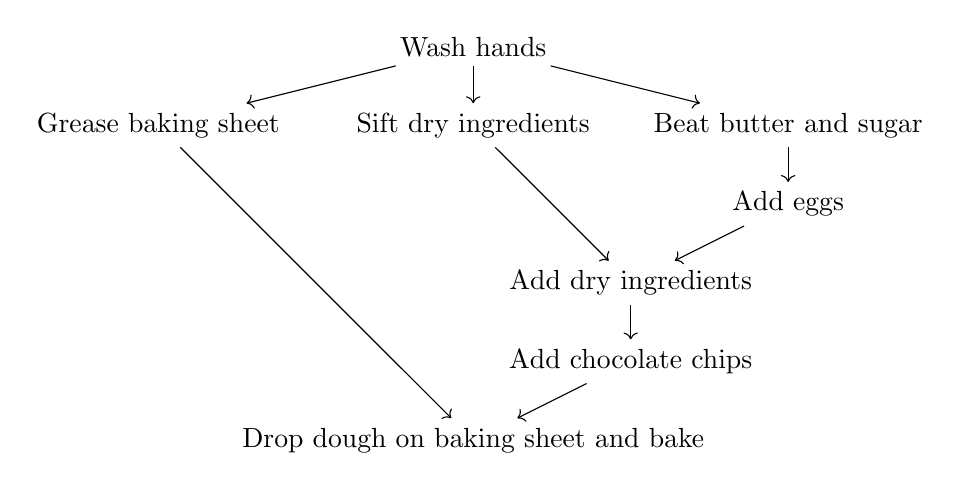
\begin{tikzpicture}
    %VARIABLES
    \pgfmathsetmacro{\spacing}{4};
    \foreach \rank/\elements/\size in {1/{Wash hands}/1, 2/{Grease baking sheet, Sift dry ingredients, Beat butter and sugar}/3,
    3/{ , , Add eggs}/3, 4/{ , Add dry ingredients}/2, 5/{ , Add chocolate chips}/2, 6/{Drop dough on baking sheet and bake}/1} {
    \foreach[count = \i] \element in \elements {\node (\element) at (\i * \spacing - \size / 2 * \spacing, -\rank) {\element};}
    }
    \foreach \j/\ls in {Wash hands/{Grease baking sheet,Sift dry ingredients,Beat butter and sugar},
    Grease baking sheet/{Drop dough on baking sheet and bake},Sift dry ingredients/{Add dry ingredients},
    Beat butter and sugar/{Add eggs},Add eggs/{Add dry ingredients},Add dry ingredients/{Add chocolate chips},
    Add chocolate chips/{Drop dough on baking sheet and bake}} {\foreach \l in \ls {\draw[->] (\j) -- (\l);}}
  \end{tikzpicture}
\end{center}

\subsubsection*{Topological Sorts of DAGs}
Consider a DAG which represents precedence constraints for a set of tasks.
Need to find an ordering which does not violate any of the precedence constraints.
A \textbf{topological} sort for a DAG is an ordering of vertices that is consistent with the edges in the graph.
\begin{itemize}
  \item If there is an edge $(u,v)$, then $u$ must appear earlier than $v$ in the topological sort.
\end{itemize}
\begin{center}
  \begin{tikzpicture}
    %VARIABLES
    \pgfmathsetmacro{\gsize}{1};
    \pgfmathsetmacro{\gnum}{3};

    \foreach[count=\i] \element in {a,b,c} {\node (\element) at (\i * 360 / \gnum:\gsize) {$\element$};}
    \foreach \j/\l in {a/c,a/b} {\draw[->] (\j) -- (\l);}
  \end{tikzpicture}
  \qquad
  \begin{tabular}{c}
    example topological sorts:         \\
    $\left\langle a,b,c\right\rangle $ \\
    $\left\langle a,c,b\right\rangle $
  \end{tabular}
\end{center}

\subsection{Equivalence relations}
A relation R is an \textbf{equivalence relation} if:
\begin{itemize}
  \item R is reflective
  \item R is transitive
  \item R is symmetric
\end{itemize}
For example:
\begin{center}
  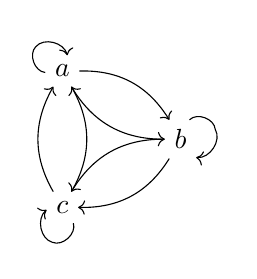
\begin{tikzpicture}
    %VARIABLES
    \pgfmathsetmacro{\gsize}{1};
    \pgfmathsetmacro{\gnum}{3};

    \foreach[count=\i] \element in {a,c,b} { %domain
        \node (\element) at (\i * 360 / \gnum:\gsize) {$\element$};
        \node (\element-) at (\i * 360 / \gnum:\gsize + 0.5) {};
        \draw[->] (\element) to[bend left=65] (\element-) to[bend left=65] (\element);
      }
    \foreach \j/\l in {a/b,b/c,a/c} { %a to b AND b to a
        \draw[->] (\j) to[bend left=20 / \gsize + 10] (\l);
        \draw[->] (\l) to[bend left=20 / \gsize + 10] (\j);
      }
  \end{tikzpicture}
  \qquad
  \begin{tikzpicture}
    %VARIABLES
    \pgfmathsetmacro{\gsize}{1};
    \pgfmathsetmacro{\gnum}{3};

    \foreach[count=\i] \element in {d,f,e} { %domain
        \node (\element) at (\i * 360 / \gnum:\gsize) {$\element$};
        \node (\element-) at (\i * 360 / \gnum:\gsize + 0.5) {};
        \draw[->] (\element) to[bend left=65] (\element-) to[bend left=65] (\element);
      }
    \foreach \j/\l in {d/f} { %a to b AND b to a
        \draw[->] (\j) to[bend left=20 / \gsize + 10] (\l);
        \draw[->] (\l) to[bend left=20 / \gsize + 10] (\j);
      }
  \end{tikzpicture}
  \qquad
  \begin{tabular}{l}
    - Reflective \\
    - Symmetric  \\
    - Transitive
  \end{tabular}
\end{center}
If $A$ is the domain of a equivalence relation and $a \in A$, then $[a]$ is called an \textbf{equivalence class},
defined to be the set of all $x \in A$, such that $a \sim x$.

For example, consider domain $\mathbb{Z}^+$ and $x \sim y$ if $x$ and $y$ have the same remainder when divided by 3.
\begin{align*}
  [0] & \text{ is } \{x \in \mathbb{Z}^+: x \mod 3 = 0\} \\
  [1] & \text{ is } \{x \in \mathbb{Z}^+: x \mod 3 = 1\} \\
  [2] & \text{ is } \{x \in \mathbb{Z}^+: x \mod 3 = 2\} \\
\end{align*}

Equivalence classes are either:
\begin{itemize}
  \item completely identical, or
  \item completely disjoint
\end{itemize}
\textbf{Theorem: Structure of Equivalence Relations}
Consider an equivalence relation on a set $A$. Let $x,y \in A$:
\begin{align*}
  \text{If}~x \sim y,~\text{then}~[x]      & = [y]                \\
  \text{If}~x \not \sim y,~\text{then}~[x] & \cap [y] = \emptyset \\
\end{align*}
\textbf{Theorem: Equivalence Relations define a Partition}
Consider and equivalence relation over a set $A$. The set of all distinct equivalence classes defines a partition of set $A$.
\begin{itemize}
  \item The term "distinct" means that if there are two equivalent classes $[a] = [b]$, then set $[a]$ is the only included one.
\end{itemize}
For example:
\begin{center}
  \begin{tikzpicture}
    %VARIABLES
    \pgfmathsetmacro{\gsize}{1};
    \pgfmathsetmacro{\gnum}{3};

    \foreach[count=\i] \element in {a,c,b} { %domain
        \node (\element) at (\i * 360 / \gnum:\gsize) {$\element$};
        \node (\element-) at (\i * 360 / \gnum:\gsize + 0.5) {};
        \draw[->] (\element) to[bend left=65] (\element-) to[bend left=65] (\element);
      }
    \foreach \j/\l in {a/b,b/c,a/c} { %a to b AND b to a
        \draw[->] (\j) to[bend left=20 / \gsize + 10] (\l);
        \draw[->] (\l) to[bend left=20 / \gsize + 10] (\j);
      }
    \node (name) at (90:\gsize+.5) {$A = \{a,b,c,d,e,f\}$}; %relation name
  \end{tikzpicture}
  \qquad
  \begin{tikzpicture}
    %VARIABLES
    \pgfmathsetmacro{\gsize}{1};
    \pgfmathsetmacro{\gnum}{3};

    \foreach[count=\i] \element in {d,f,e} { %domain
        \node (\element) at (\i * 360 / \gnum:\gsize) {$\element$};
        \node (\element-) at (\i * 360 / \gnum:\gsize + 0.5) {};
        \draw[->] (\element) to[bend left=65] (\element-) to[bend left=65] (\element);
      }
    \foreach \j/\l in {d/f} { %a to b AND b to a
        \draw[->] (\j) to[bend left=20 / \gsize + 10] (\l);
        \draw[->] (\l) to[bend left=20 / \gsize + 10] (\j);
      }
  \end{tikzpicture}
  \qquad
  \begin{tabular}{l}
    $[a] = \{a,b,c\}$ \\
    $[d] = \{d,f\}$   \\
    $[e] = \{e\}$     \\
  \end{tabular}
\end{center}

\subsection{N-ary relations and relational databases}
A binary relation can be generalized to more than two sets. A relation on $n$ sets is called an \textbf{N-nary Relation}.
For example:
\begin{align*}
  (w,x,y,z)  & \in \mathbb{R}^4~\text{such that}~wx=yz                                                  \\
  (3,12,4,9) & ~\text{would be in the relation because}                 & 3 \cdot 12 & = 4 \cdot 9      \\
  (3,8,5,6)  & ~\text{would \underline{not} be in the relation because} & 3 \cdot 8  & \not = 5 \cdot 6
\end{align*}

\subsubsection*{Databases}
A database is a large collection of data records that is searched and manipulated by a computer.
The \textit{regional database model} stores data records as relations.

The type of data stored in each entry of the n-tuple is called an \underline{attribute}.

A \underline{query} to a database is a request for a particular set of data.

A \underline{key} is an attribute or set of attributes that uniquely identifies each n-tuple in the databases.

For example, Airlines use the combination of flight number, date, and departure time to uniquely identify a flight.

\subsubsection*{Selection}
The \textbf{selection} operation chooses n-tuples from a relational database that satisfies particular conditions on their attributes.
For example:
\begin{center}
  \begin{tabular}{cccc}
    \# boxes & Order Date & Complete? & Client City      \\
    \hline
    8        & 6/19/2013  & NO        & Irvine           \\
    12       & 6/20/2013  & YES       & Huntington Beach \\
    15       & 6/20/2013  & YES       & Huntington Beach \\
    21       & 6/20/2013  & NO        & Irvine           \\
    3        & 6/21/2013  & NO        & Costa Mesa
  \end{tabular}
\end{center}
Search[Complete=NO]
\begin{center}
  \begin{tabular}{cccc}
    \# boxes & Order Date & Complete? & Client City \\
    \hline
    8        & 6/19/2013  & NO        & Irvine      \\
    21       & 6/20/2013  & NO        & Irvine      \\
    3        & 6/21/2013  & NO        & Costa Mesa
  \end{tabular}
\end{center}
Search[Complete=NO $\land$ Data $<$ 6/21/2013]
\begin{center}
  \begin{tabular}{cccc}
    \# boxes & Order Date & Complete? & Client City \\
    \hline
    8        & 6/19/2013  & NO        & Irvine      \\
    21       & 6/20/2013  & NO        & Irvine
  \end{tabular}
\end{center}

\subsubsection*{Projection}
The \textbf{projection} operation takes a subset of the attributes and deletes all other attributes in each of the n-tuples.
For example:
\begin{center}
  \begin{tabular}{cccc}
    \# boxes & Order Date & Complete? & Client City      \\
    \hline
    8        & 6/19/2013  & NO        & Irvine           \\
    12       & 6/20/2013  & YES       & Huntington Beach \\
    15       & 6/20/2013  & YES       & Huntington Beach \\
    21       & 6/20/2013  & NO        & Irvine           \\
    3        & 6/21/2013  & NO        & Costa Mesa
  \end{tabular}
\end{center}
Project[Order Date, Client City]
\begin{center}
  \begin{tabular}{cc}
    Order Date & Client City      \\
    \hline
    6/19/2013  & Irvine           \\
    6/20/2013  & Huntington Beach \\
    6/20/2013  & Irvine           \\
    6/21/2013  & Costa Mesa
  \end{tabular}
\end{center}
Select[Complete=NO], Project[City]
\begin{center}
  \begin{tabular}{c}
    Client City \\
    \hline
    Irvine      \\
    Costa Mesa
  \end{tabular}
\end{center}
\section{Computation}
\subsection{An introduction to algorithms}
An algorithm is a step by step method for solving a problem. It usually includes:
\begin{itemize}
  \item name
  \item brief description
  \item description of input
  \item description of output
  \item sequence of steps to follow
\end{itemize}
Algorithms are often described in \textbf{pseudocode}

\subsubsection*{Assignment operator}
\begin{lstlisting}
  x := y
\end{lstlisting}

\subsubsection*{Return statement}
\begin{lstlisting}
  Return(value)
\end{lstlisting}

\subsubsection*{If-else statement}
\begin{lstlisting}
  If(x = 5), y := 7

  If(condition)             If(condition)
    Step 1                    Step(s)
    Step 2                  Else
    ...                       Step(s)    
    Step n                  End-if
  End-if
\end{lstlisting}

\subsubsection*{For-loop}
\begin{lstlisting}
  For i = s to t    <- first value is s, then s+1, until t is reached
    Step(s)
  End-for
\end{lstlisting}

\subsubsection*{While-loop}
\begin{lstlisting}
  While(condition)
    Step(s)
  End-while
\end{lstlisting}

\subsubsection*{Nested Loops}
\begin{lstlisting}
  Input: sequence a_1, ..., a_n; n

  count := 0
  For i = 1 to n-1
    For j = i+1 to n
      If(a_i = a_j) count := count+1
    End-for
  End-for

  Return(count)
\end{lstlisting}

\subsection{Asymptotic growth of functions}
Consider $f: \mathbb{Z}^+ \rightarrow \mathbb{R}^{\geq}$, where $\mathbb{R}^{\geq}$ denotes the set of non-negative real numbers.
\textbf{Asymptotic growth} of a function $f$ is a measure of how fast the object $f(n)$ grows as the input $n$ grows.
Classification of functions $\mathcal{O}, \Omega,$ and $\Theta$ provide a way to concisely characterize the growth of a function.
\[
  f = \mathcal{O}(g)~~\text{"$f$ is Oh of $g$"}
\]

\subsubsection*{Constant factors}
\begin{align*}
  7n^3 & \rightarrow 7 \text{ is constant factor} \\
  5n^2 & \rightarrow 5 \text{ is constant factor} \\
  3    & \rightarrow 3 \text{ is constant factor}
\end{align*}

\subsubsection*{$\mathcal{O}$ notation}
Let $f$ and $g$ be functions from $\mathbb{Z}^+$ to $\mathbb{R}^{\geq}$.
Then $f=\mathcal{O}(g)$ if there is are positive real numbers $c$ and $n_0$ such that for any $n \in \mathbb{Z}^+$ such that $n \geq n_0$,
\[
  f(n) \leq c \cdot g(n)
\]
Constants $c$ and $n_0$ are said to be a \textit{witness} to the fact $f=\mathcal{O}(g)$

\subsubsection*{$\Omega$ notation}
Let $f$ and $g$ be functions from $\mathbb{Z}^+$ to $\mathbb{R}^{\geq}$.
Then $f=\Omega(g)$ if there is are positive real numbers $c$ and $n_0$ such that for any $n \in \mathbb{Z}^+$ such that $n \geq n_0$,
\[
  f(n) \geq c \cdot g(n)
\]
$f=\Omega(g)$ is read "$f$ is Omega of $g$"

\subsubsection*{Theorem: Relationship of $\mathcal{O}$-notation and $\Omega$-notation}
Let $f$ and $g$ be functions from $\mathbb{Z}^+$ to $\mathbb{R}^{\geq}$. Then $f=\Omega(g) \iff g = \mathcal{O}(f)$

\subsubsection*{$\Theta$ notation}
Let $f$ and $g$ be functions from $\mathbb{Z}^+$ to $\mathbb{R}^{\geq}$.
\[
  f = \Theta(g) \text{ if}: f = \mathcal{O}(g) \land f = \Omega(g)
\]
\begin{itemize}
  \item $f = \Theta(g)$ is read "$f$ is Theta of $g$"
  \item if $f = \Theta(g)$, then $f$ is said to be the \textit{order of} $g$.
\end{itemize}

\subsubsection*{Theorem: Asymptotic Growth of Polynomials}
Let $p(n)$ be a degree-$k$ polynomial of the form
\[
  p(n) = a_{k}n^{k} + a_{k-1}n^{k-1} + \cdots + a_{1}n + a_0 \text{ where } a_k > 0 \\
\]
Then $p(n)$ is $\Theta(n^k)$

\subsubsection*{Asymptotic Growth of Logarithm Functions with Different Bases}
Let $a$ and $b$ be two real numbers greater than 1. Then
\[
  \log_{a}n = \Theta(\log_{b}n)
\]
This is because of the fact that
\[
  \log_{a}n = \log_{a}b \cdot \log_{b}n, \text{ for } a,b > 1
\]
\textit{
  when a function is said to be the $\mathcal{O}$ or $\Omega$ of a logarithm function,
  the base is often omitted because it is understood that as long as the base is greater than 1,
  the value of the base does not matter.
}

\subsubsection*{Growth rate of common functions}
Constant Functions
\begin{itemize}
  \item function that does not depend on $n$ at all
  \item any constant function is $\Theta(1)$
\end{itemize}
Linear
\begin{itemize}
  \item $\Theta(n)$
\end{itemize}
\begin{center}
  \begin{tabular}{l|c}
    Function                                   & Name        \\
    \hline
    $\Theta(1)$                                & Constant    \\
    $\Theta(\log\log n)$                       & Log Log     \\
    $\Theta(\log n)$                           & Logarithmic \\
    $\Theta(n)$                                & Linear      \\
    $\Theta(n \log n)$                         & $n \log n$  \\
    $\Theta(n^2)$                              & Quadratic   \\
    $\Theta(n^3)$                              & Cubic       \\
    $\Theta(n^m)~\text{for}~m\in \mathbb{Z}^+$ & Power       \\
    $\Theta(c^n)~\text{for}~c>1$               & Exponential \\
    $\Theta(n!)$                               & Factorial
  \end{tabular}
\end{center}

\subsubsection*{Rules about Asymptotic Growth}
Let $f$, $g$, and $h$ be functions from $\mathbb{Z}^+$ to $\mathbb{R}^{\geq}$.
\begin{itemize}
  \item if $f=\mathcal{O}(h)$ and $g=\mathcal{O}(h)$, then $f+g=\mathcal{O}(h)$
  \item if $f=\Omega(h)$ and $g=\Omega(h)$, then $f+g=\Omega(h)$
  \item if $f=\mathcal{O}(g)$, $c \cdot f = \mathcal{O}(g)$, $c\in \mathbb{R}^{\geq}$
  \item if $f=\Omega$, $c \cdot f = \Omega(g)$, $c\in \mathbb{R}^{\geq}$
  \item if $f=\mathcal{O}(g)$ and $g=\mathcal{O}(h)$, then $f=\mathcal{O}(h)$
  \item if $f=\Omega(g)$ and $g=\Omega(h)$, then $f=\Omega(h)$
\end{itemize}

\subsection{Analysis of algorithms}
Resources an algorithm requires to run
\begin{itemize}
  \item time, called \textit{time complexity}
  \item space, called \textit{space complexity}
  \item Together called \textbf{computational complexity}
\end{itemize}
\begin{lstlisting}
  ComputeSum
  Input: a_1,a_2,...,a_n  (n is length of sequence)
  Output: the sum of the numbers in the sequence
  sum := 0                  | 1 assignment operation
  For i = 1 to n            | loop iterated n times
    sum := sum + a_i        |   for loop test and increments (2 operations)
  End-for                   |   1 addition and 1 assignment (2 operations)
  Return(sum)               | 1 op for return statement
\end{lstlisting}
\begin{align*}
  f(n) & = 1 + n[2+2] + 1 \\
       & = 1 + 4n + 1     \\
       & = 4n + 2         \\
       & = \mathcal{O}(n)
\end{align*}

\subsubsection*{Growth rates for different input sizes}
\[
  \begin{matrix}
    f(n)       & n=10      & n=50      & n=100                & n=1000                  & \cdots \\
    \log_{2}n  & 3.3 \mu s & 5.6 \mu s & 6.6 \mu s            & 10 \mu s                & \cdots \\
    n          & 10 \mu s  & 50 \mu s  & 100 \mu s            & 1000 \mu s              & \cdots \\
    n\log_{2}n & .03 ms    & .28 ms    & .66 ms               & 10 ms                   & \cdots \\
    n^2        & .1 ms     & 2.5 ms    & 10 ms                & 1 s                     & \cdots \\
    n^3        & 1 ms      & .125 s    & 1 s                  & 16.7 min                & \cdots \\
    2^n        & 1 ms      & 35.7 yrs  & 4 \times 10^{16} yrs & 3.4 \times 10^{287} yrs & \cdots \\
  \end{matrix}
\]

\subsubsection*{Worst-case analysis}
Worst-case analysis evaluates the time complexity on the input which takes the longest time.
\begin{itemize}
  \item upper bound: use $\mathcal{O}$-notation
        \subitem upper bound must apply for every input of size $n$
  \item lower bound: use $\Omega$-notation
        \subitem lower bound need only apply for one possible input of $n$
\end{itemize}
Average-case analysis takes an average running time of algorithm on random inputs.
\begin{lstlisting}
  For(----)
    operations      -> linear (n)
  End-for

  For(----)
    For(----)
      operations    -> quadratic (n^2)
    End-for
  End-for

  For(----)
    For(----)
      For(----)
        operations  -> cubic (n^3)
      End-for
    End-for
  End-for
\end{lstlisting}
and so on. An algorithm runs in \underline{polynomial time} if its time complexity is $\mathcal{O}^k$ for some fixed constant $k$.
An algorithm is considered "efficient" if it runs in polynomial time. For example,
\begin{align*}
  \mathcal{O}(n^5)        & ~\text{is "efficient"}                 \\
  \mathcal{O}(n^{\log n}) & ~\text{is \underline{not} "efficient"}
\end{align*}
\subsection{Finite state machines}
A \textbf{finite state machine} consists of a finite set of states,
with transitions between states triggered by different input actions.
A finite state machine is sometimes called \textit{finite state automation}.
\begin{center}
  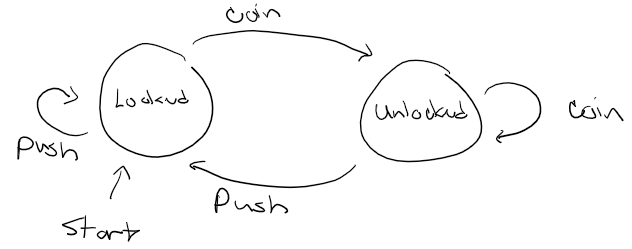
\includegraphics[width=.6\linewidth]{resources/coin_push.png}

  states: $Q =$\{locked, unlocked\}
\end{center}
The reaction of a finite state machine to the input received is denoted by a \textbf{transitive function},
often denoted by the symbol '$\delta$'
\[
  \delta([\text{state}],[\text{action}]) = [\text{state}]
\]
In the case of the coin machine,
\[
  \delta(\text{Locked}, \text{Coin}) = \text{Unlocked}
\]
State transition table:
\begin{itemize}
  \item rows represent current state
  \item columns represent possible inputs
  \item each entry for a particular row and column indicate the new state resulting from that state/input combination
\end{itemize}
For example, the state transition table for the coin machine is
\begin{center}
  \begin{tabular}{c|cc}
             & Coin     & Push   \\
    \hline
    Locked   & unlocked & locked \\
    Unlocked & unlocked & locked
  \end{tabular}
\end{center}

\subsubsection*{Components of a Finite State Machine}
\begin{center}
  \begin{tabular}{c|l}
    Notation                           & Description              \\
    \hline
    $Q$                                & finite set of states     \\
    $q_0 \in Q$                        & $q_0$ is the start state \\
    $I$                                & finite set of actions    \\
    $\delta: Q \times I \rightarrow Q$ & transition function
  \end{tabular}
\end{center}

\subsubsection*{FSM with Output}
\begin{align*}
  Q & = \{q_0, q_5, q_{10}, q_{15}, q_{20}\}                           \\
  I & = \{\text{NICKLE}, \text{DIME}, \text{BUY}\}                     \\
  O & = \{\text{Gumball}, \text{Return}, \text{Message}, \text{None}\}
\end{align*}
\begin{center}
  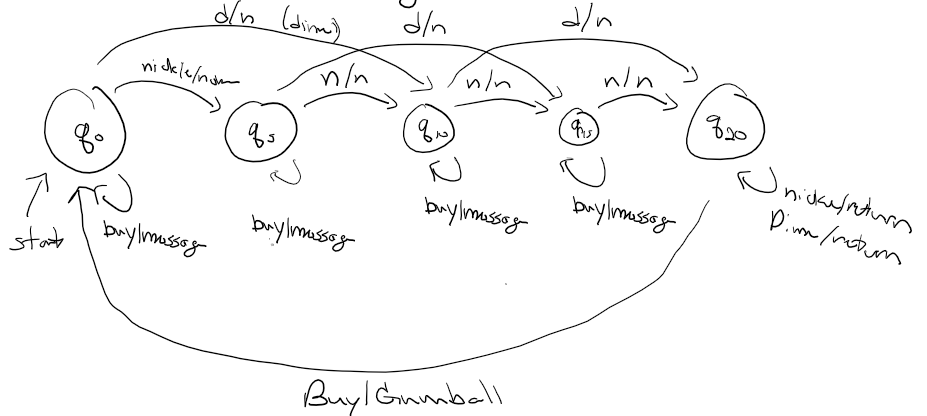
\includegraphics[width=.6\linewidth]{resources/fsm_with_output.png}
\end{center}
An \underline{accepted state} is a state that is okay to end in.
\[
  A \subseteq Q, \text{ Accepted states are a subset of the total states}
\]
Example, recognizing valid password
\begin{center}
  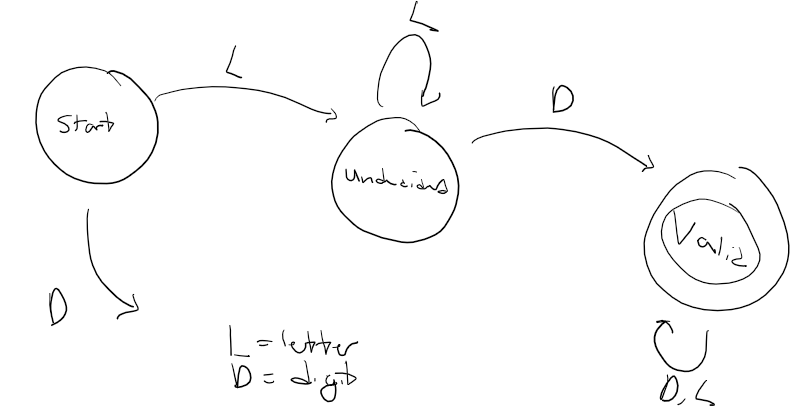
\includegraphics[width=.6\linewidth]{resources/fsm_password.png}

  A valid password must begin with a letter and contain at least one digit.
\end{center}

\subsection{Turing machines}
FSMs are unable to solve even simple computational tasks such as determining whether a binary string has more 0's than 1's.

\subsubsection*{Church-Turing conjecture}
Any problem that can be solved efficiently on any computing device can be solved efficiently by a Turing Machine.

\subsubsection*{Definition of a Turing Machine}
\begin{itemize}
  \item memory is a 1-dimensional tape. \\
        \begin{tikzpicture}
          \pgfmathsetmacro{\x}{0.5};
          \pgfmathsetmacro{\y}{0.5};
          \pgfmathsetmacro{\vset}{0};

          \foreach[count=\i] \element in {a,b,b,b,a,b,a,b,a,b,b,b,a} {
              \draw (\i * \x,0) rectangle ++(\x,\y);
              \node[anchor=south] (\element) at (\i*\x + \x * 0.5, \vset) {$\element$};
            }
        \end{tikzpicture} \\
        example tape for $\{a,b,*\}$
  \item blank symbol (represented by a $*$ symbol)
  \item a \underline{configuration} consists of the contents of the tape, the current state,
        and the tape cell to which the head is currently pointing \\
        \begin{tikzpicture}
          \pgfmathsetmacro{\x}{0.5};
          \pgfmathsetmacro{\y}{0.5};
          \pgfmathsetmacro{\vset}{0};
          \pgfmathsetmacro{\qset}{7};

          \foreach[count=\i] \element in {a,b,b,b,a,b,a,b,a,b,b,b,a} {
              \draw (\i * \x,0) rectangle ++(\x,\y);
              \node[anchor=south] (\element) at (\i*\x + \x * 0.5, \vset) {$\element$};
            }
          \draw[very thick] (\qset*\x, \y + 0.1) rectangle ++(\x,\y);
          \node[anchor=south] (q) at (\qset*\x + \x*0.5, \y + 0.1) {$q$};
        \end{tikzpicture}
  \item action is determined by a transition function $\delta$
\end{itemize}
Input to Turing Machine is the Input Alphabet, denoted by $\Sigma$,
which much be a subset of the tape alphabet $\Gamma$
\[
  \Sigma \subset \Gamma
\]

\subsubsection*{Components of a Turing Machine}
\begin{center}
  \begin{tabular}{r|l}
    Notation                                                              & Description                                    \\
    \hline
    $Q$                                                                   & finite set of states                           \\
    $\Gamma$                                                              & finite set of tape symbols                     \\
    $\Sigma \subset \Gamma$                                               & A subset of the tape symbols are input symbols \\
    $q_0 \in Q$                                                           & $q_0$ is the start state                       \\
    $q_{acc} \in Q$                                                       & $q_{acc}$ is the accept state                  \\
    $q_{rej} \in Q$                                                       & $q_{rej}$ is the reject state                  \\
    $\delta : Q \times \Gamma \rightarrow Q \times \Gamma \times \{L,R\}$ & Transition Function
  \end{tabular}
\end{center}
Additional Rules
\begin{itemize}
  \item if Turing machine reaches the accept state from a particular input $x$, the Turing machine \textbf{accepts} $x$
  \item if Turing machine reaches the reject state from a particular input $x$, the Turing machine \textbf{rejects} $x$
  \item if Turing machine \textit{accepts} or \textit{rejects} $x$, then the Turing machine \textbf{Halts} on $x$
\end{itemize}
Turing machine that accepts strings with 2 $b$'s
\begin{center}
  \begin{tabular}{c|ccc}
          & $a$         & $b$             & $*$             \\
    \hline
    $q_0$ & $(q_0,a,R)$ & $(q_1,b,R)$     & $(q_{rej},*,L)$ \\
    $q_1$ & $(q_1,a,R)$ & $(q_{acc},b,R)$ & $(q_{rej},*,L)$
  \end{tabular}
\end{center}
\begin{center}
  \begin{tabular}{c}
    \begin{tikzpicture}
      \pgfmathsetmacro{\x}{0.5};
      \pgfmathsetmacro{\y}{0.5};
      \pgfmathsetmacro{\vset}{0};
      \pgfmathsetmacro{\qset}{1};

      \foreach[count=\i] \element in {a,b,b,a,*} {
          \draw (\i * \x,0) rectangle ++(\x,\y);
          \node[anchor=south] (\element) at (\i*\x + \x * 0.5, \vset) {$\element$};
        }
      \draw[very thick] (\qset*\x, \y + 0.1) rectangle ++(\x,\y);
      \node[anchor=south] (q) at (\qset*\x + \x*0.5, \y + 0.1) {$q_0$};
    \end{tikzpicture} \\
    $\uparrow$ Halts and accepts
  \end{tabular}
  \qquad
  \begin{tabular}{c}
    \begin{tikzpicture}
      \pgfmathsetmacro{\x}{0.5};
      \pgfmathsetmacro{\y}{0.5};
      \pgfmathsetmacro{\vset}{0};
      \pgfmathsetmacro{\qset}{1};

      \foreach[count=\i] \element in {a,b,a,a,*} {
          \draw (\i * \x,0) rectangle ++(\x,\y);
          \node[anchor=south] (\element) at (\i*\x + \x * 0.5, \vset) {$\element$};
        }
      \draw[very thick] (\qset*\x, \y + 0.1) rectangle ++(\x,\y);
      \node[anchor=south] (q) at (\qset*\x + \x*0.5, \y + 0.1) {$q_0$};
    \end{tikzpicture} \\
    $\uparrow$ Halts and rejects
  \end{tabular}
\end{center}
Transition function for Turing machine that recognizes powers of 2:
\begin{center}
  \begin{tabular}{c|ccc}
    -           & $a$               & $x$               & $*$               \\
    \hline
    $q_0$       & $(q_{first},*,R)$ & $(q_{rej},*,R)$   & $(q_{rej},x,R)$   \\
    $q_{first}$ & $(q_{even},x,R)$  & $(q_{first},x,R)$ & $(q_{first},*,R)$ \\
    $q_{even}$  & $(q_{odd},a,R)$   & $(q_{even},x,R)$  & $(q_{first},*,R)$ \\
    $q_{odd}$   & $(q_{even},x,R)$  & $(q_{odd},x,R)$   & $(q_{first},*,R)$ \\
    $q_{ret}$   & $(q_{ret},a,R)$   & $(q_{rej},x,R)$   & $(q_{first},*,R)$ \\
  \end{tabular}
\end{center}

\subsection{Decision problems and languages}
\begin{center}
  \begin{tikzpicture}
    %VARIABLES
    \pgfmathsetmacro{\gsize}{1};
    \pgfmathsetmacro{\gnum}{4};

    \foreach[count=\i] \element in {1,2,3,4} { %domain
        \node (\element) at (\i * 360 / \gnum:\gsize) {$\element$};
      }
    \foreach \j/\ls in {1/{2,4},3/{1,4}} {\foreach \l in \ls {\draw[->] (\j) -- (\l);}}
  \end{tikzpicture}
  \begin{tabular}{r|l}
    Symbol set     & ${()~,~;~0~1~2~3~4~5~6~7~8~9}$ \\
    Graph encoding & $4;(1,2)(1,4)(3,1)(3,4)$
  \end{tabular}
\end{center}
Turing Machine can only accept or reject on input.
This limits the class of problems answerable by a turing machine to \textbf{yes} or \textbf{no} problems.
\begin{itemize}
  \item \textbf{Decision Problem}: given a boolean expression, is there
        an assignment to the boolean expression that causes the expression to evaluate to 1?
  \item \textbf{Search Problem}: given a boolean expression, find an assignment to the boolean
        expression that causes the expression to evaluate to 1 if one exists,
        or output that no such assignment exists.
\end{itemize}
If $\Sigma$ is a finite alphabet, then a subset of $\Sigma^*$ is called a \textit{language} over $\Sigma$.

\subsubsection*{Language computed by a Turing Machine}
Let $\Sigma$ denote a finite alphabet and let $L$ be a language over $\Sigma$.
A turing machine $M$ \textbf{computes language L}, or \textbf{decides language L}
if for every $x \in \Sigma$, if $x \in L$, then $M$ rejects $x$ in a finite number of steps.
\begin{itemize}
  \item \textbf{Time Complexity} is measured by how many steps taken by a Turing machine on a particular input.
  \item \textbf{Space Complexity} is measured by the number of tape cells that the turing machine uses in the
        course of it execution on a particular input.
\end{itemize}
A language is \textit{incomputable} if there is no turing machine that computes the language.
\section{Induction and Recursion}
\subsection{Sequences}
A \textbf{sequence} is a special type of function in which the domain
is the set of consecutive integers.

When a function is specified as a sequence, using subscripts to denote input
is more common, so $g_k$ is used instead of $g(k)$

A value $g_k$ is called a \textbf{term}, and $k$ is the \textit{index} of $g_k$

For example:
\begin{align*}
  g_1 & = 3.67 & g_2 & = 2.88 \\
  g_3 & = 3.25 & g_4 & = 3.75
\end{align*}
\[
  g(k) = 3.67, 2.88, 3.25, 3.75
\]

An entire sequence is denoted by $\{gk\}$, whereas $g_k$ is used to denote a
single term in the sequence.

A sequence commonly starts with $0$ or $1$, but it could be \textit{any} integer.
\subsubsection*{Finite sequence}
A sequence with a finite domain is a \textbf{finite sequence}.
In a finite sequence, there is an \textit{initial index $m$} and a \textit{final index $n$}.
\subsubsection*{Infinite sequence}
A sequence with an infinite domain is a \textbf{infinite sequence}.
In an infinite sequence, there is an \textit{initial index m} and the sequence
is defined for indices $k \geq m$:
\[
  a_m, a_{m+1}, a_{m+2}, a_{m+3}, \ldots
\]
A sequence can be specified by an \textbf{explicit formula}, such as $d_k = 2^k$
for $k \geq 1$.
\[
  \{d_k\} = 2,4,8,16, \ldots
\]
\subsubsection*{Increasing and Decreasing Sequences}
\begin{itemize}
  \item a sequence is \textit{increasing} if for every two consecutive indices, $k$
        and $k+1$, $a_k < a_{k+1}$
  \item a sequence is \textit{non-decreasing} if for every two consecutive indices, $k$
        and $k+1$, $a_k \leq a_{k+1}$
\end{itemize}
For example,
\begin{align*}
  2 < 4 < 5 < 6          & ~\text{increasing \textit{and} non-decreasing}     \\
  2 \leq 4 \leq 5 \leq 6 & ~\text{non-decreasing \textit{but} not increasing}
\end{align*}
\textit{The same relationship can be said for \textbf{decreasing} and \textbf{non-increasing}}.
\subsubsection*{Geometric Sequences}
A \textbf{geometric sequence} is a sequence of real numbers where each term is found by taking
the previous term and multiplying it by a fixed number called the \textbf{common ratio}.

For example, with an \textit{initial term}: 4, and \textit{common ratio}: $\frac{1}{2}$,
\[
  4,2,\frac{1}{2},\frac{1}{4}, \ldots
\]
\subsubsection*{Arithmetic Sequence}
An \textbf{arithmetic sequence} is a sequence of real numbers where each term after the initial
term is found by taking the previous term and adding a fixed number called the \textbf{common difference}.

For example, with an \textit{initial value}: 2, and \textit{common difference}: 3,
\[
  2,5,8,11, \ldots
\]

\subsection{Recurrence relations}
A rule that defines a term $a_n$ as a function of previous terms in the sequence is called a
\textbf{recurrence relation}

For example,
\begin{align*}
  a_0 & = a~\text{initial value} \\
  a_n & = d + a_{n-1}
\end{align*}
Fibonacci Sequence:
\begin{align*}
  f_0 & = 0                                     \\
  f_1 & = 1                                     \\
  f_n & = f_{n-1} + f_{n-2}~\text{for}~n \geq 2 \\
\end{align*}
A \textbf{dynamical system} is a system that changes over time. The state of the system
at any point is determined by a set of well-defined rules that depend on the past states
of the system.

\subsection{Summations}
\textbf{Summation Notation} is used to express the sum of terms in a numerical sequence.
\[
  \sum_{i=s}^{t} a_i = a_{s} + a_{s+1} + \ldots + a_t
\]
\begin{center}
  \begin{tabular}{l}
    $i$ is the \textit{index}       \\
    $s$ is the \textit{lower limit} \\
    $t$ is the \textit{upper limit}
  \end{tabular}
\end{center}
Any variable name could be used for index, but $i,j,k$ and $\ell$
are most common.
\begin{align*}
  \sum_{j=1}^{4} j^3    & :~\text{summation form} \\
  1^3 + 2^3 + 3^3 + 4^3 & :~\text{expanded form}
\end{align*}
\[
  \sum_{k=m}^{n} a_k = \sum_{k=m}^{n-1} a_k + a_n,~\text{for}~n>m
\]
\[
  \sum_{j=1}^{n} (j+2)^3 = \sum_{k=1}^{n} (k+2)^3 = \sum_{i=3}^{n+2} i^3
\]
\subsubsection*{Closed Form}
A \textbf{closed form} for a mathematical sum expresses the value of the sum without
summation notation. For example,
\[
  \sum_{k=0}^{n-1} (a+kd) = an + \frac{d(n-1)n}{2}
\]
\textbf{Arithmetic Sequence Closed Form}:
\[
  \sum_{k=0}^{n-1} (a+kd) = an + \frac{d(n-1)n}{2}
\]
\textbf{Geometric Sequence Closed Form}:
\[
  \sum_{k=0}^{n-1} (a \cdot r^k) = \frac{a(r^n-1)}{r-1}
\]

\subsection{Mathematical induction}
Two Components of an inductive proof:
\begin{itemize}
  \item Base Case:
        \subitem establishes that the theorem is true for the first value in the sequence
  \item Inductive Step:
        \subitem establishes that if the theorem is true for $k$, then the theorem holds for $k+1$
\end{itemize}
\[
  \text{For a}~k \in \mathbb{Z}^+,~s(k) \implies s(k+1)
  \iff [s(1) \implies s(2) \implies s(3) \implies s(4) \implies \cdots]
\]
The supposition that $s(k)$ is true is called the \underline{inductive hypothesis}.

\subsection{More inductive proofs}
Explicit formula for a sequence defined by a recurrence relation
\begin{align*}
  \{g_n\}:~g_0 & =1,~g_n=3g_{n-1} + 2n~\text{then for any $n \geq 0$,} \\
  g_n          & = \frac{5}{2} \cdot 3^n - n - \frac{3}{2}
\end{align*}
\begin{proof}
  by induction on $n$. \\
  Base Case: $n=0$
  \begin{align*}
    g_o & = \frac{5}{2} \cdot 3^0 - 0 - \frac{3}{2} = 1    \\
    g_0 & = 1~\checkmark\quad\text{(by initial condition)}
  \end{align*}
  Inductive Step: assume for any integer $k\geq0$, assume that $g_k=\frac{5}{2} \cdot 3^k-k-\frac{3}{2}$ is true.\\
  For $k+1$:
  \begin{align*}
    g_{k+1} & = 3g_{k} + 2(k+1)\quad\text{by definition}                                  \\
            & = 3(\frac{5}{2}3^k-k-\frac{3}{2})+2(k+1)\quad\text{by induction hypothesis} \\
            & = \frac{5}{2}3^{k+1}-3k-\frac{9}{2}+2k+2                                    \\
            & = \frac{5}{2}3^{k+1}-k-\frac{5}{2}                                          \\
            & = \frac{5}{2}3^{k+1}-(k+1)-\frac{5}{2}\quad\text{by algebra}
  \end{align*}
  $\therefore g_n = \frac{5}{2} \cdot 3^n - n - \frac{3}{2}$, for all $n \in \mathbb{Z}^\geq$
\end{proof}

\subsection{Strong induction and well-ordering}
The \textbf{principle of strong induction} assumes the fact to be proven holds for all values
less than or equal to $k$ and proves the fact holds for $k+1$
\begin{center}
  \begin{tabular}{cllll}
    \multicolumn{5}{c}{Inductive Step for Weak Induction}                  \\
    \hline
    \multicolumn{5}{c}{For all $k\geq1,~S(k) \implies S(k+1)$}             \\
    $k=1$    & $S(1)\implies$ & $S(2)$         &                &          \\
    $k=2$    &                & $S(2)\implies$ & $S(3)$         &          \\
    $k=3$    &                &                & $S(3)\implies$ & $S(4)$   \\
    $\vdots$ &                &                &                & $\ddots$
  \end{tabular}
  \qquad
  \begin{tabular}{cllll}
    \multicolumn{5}{c}{Inductive Step for Strong Induction}                                       \\
    \hline
    \multicolumn{5}{c}{For all $k\geq1,~S(0) \land S(1) \land \ldots \land S(k) \implies S(k+1)$} \\
    $k=1$    & $S(1)\implies$    & $S(2)$            &                &                           \\
    $k=2$    & $S(1)\quad\land $ & $S(2)\implies$    & $S(3)$         &                           \\
    $k=3$    & $S(1)\quad\land $ & $S(2)\quad\land $ & $S(3)\implies$ & $S(4)$                    \\
    $\vdots$ &                   &                   &                & $\ddots$
  \end{tabular}
\end{center}
for $n\geq0,~f_n \leq 2^n$
\begin{proof}
  By Strong Induction of $n$

  Base Case:
  \begin{align*}
    n & = 0:~f_0 = 0 \leq 2^0~\checkmark \\
    n & = 1:~f_1 = 1 \leq 2^1~\checkmark \\
  \end{align*}
  Inductive Step:

  For $k\geq1$, suppose that for any $j$ in the range from $0$ through $k$, $f_k\leq2^j$.
  We will prove that $f_{k+1}\leq2^{k+1}$.

  Since $k\geq1$, then $k-1\geq0$. Therefore both $k$ and $k-1$ fall in the range from
  $0$ through $k$, and by the induction hypothesis $f_{k-1}\leq2^{k-1}$ and $f_k\leq2^k$
  \begin{align*}
    f_{k+1} & = f_k + f_{k-1}              &  & \text{by definition}           \\
            & \leq 2^k + 2^{k-1}           &  & \text{by inductive hypothesis} \\
            & \leq 2^k + 2^{k-1} + 2^{k-1} &  & \text{since $2^{k-1} \geq 0$}  \\
            & \leq 2^k + 2 \cdot 2^{k-1}                                       \\
            & \leq 2^k + 2^k                                                   \\
            & \leq 2 \cdot 2^k                                                 \\
    f_{k+1} & \leq 2^{k+1}                 &  & \text{by algebra}
  \end{align*}
  $\therefore f_{k+1} \leq 2^{k+1}$
\end{proof}

\subsection{Loop invariants}
\subsubsection*{Program Verification}
\begin{itemize}
  \item formally proving that programs perform correctly
  \item behavior is correct if:
        \subitem a pre-condition is true before the program starts
        \subitem a post-condition is true before the program ends
\end{itemize}
\subsubsection*{Loop Invariants for While Loops}
A loop invariant is an assertion that is true before each iteration of a loop.

\subsection{Recursive definitions}
In a recursive definition of a function, the value of the function is defined in term
of the output of the function on smaller input values.

For examples, the factorial:
\begin{align*}
  n!   & = f(n)\quad\text{such that}   \\
  f(0) & = 1                           \\
  f(1) & = n \cdot f(n-1) for n \geq 1
\end{align*}

\subsection{Structural induction}
\textbf{Structural induction} is a type of induction used to prove theorem about recursively
defined sets that follow the structure of the recursive definition.

For example, balanced parenthesis
\begin{align*}
  \text{right}[~))()~]  & = 3 & \text{left}[~)))~] = 0 \\
  \text{left}[~((()))~] & = 3
\end{align*}
Recursive definition for the set of properly nested parenthesis:
\begin{center}
  \begin{tabular}{r|c}
    Basis           & $()\in P$           \\
    Recursive Rules & If $u,v\in P$, then \\
    1               & $(u) \in P$         \\
    2               & $uv \in P$
  \end{tabular}
\end{center}
\textit{Theorem}: If string $x\in P$, then left$[~x~] =$ right $[~x~]$
\begin{proof}
  by structural induction

  \textbf{Base Case}: $() \in P$
  \[
    \text{left}[~()~] = \text{right}[~()~] = 1
  \]

  \textbf{Inductive Step}: If $x\in P$, then $x$ was constructed by apply a sequence
  of recursive rules starting with the string $()$ given in the basis.

  We consider two case, depending on the last recursive rule that was applies to construct $x$.

  \textbf{Case 1} Rules 1 was the last applied to construct $x$.
  Then $x = (u)$, where $u\in P$. We assume that left$[~u~] =$ right $[~u~]$.
  \begin{align*}
    \text{left}[~x~] & = \text{left}[~(u)~]    &  & \text{because $x = (u)$}               \\
                     & = 1 + \text{left}[~u~]  &  & \text{$(u)$ has one more $($ than $u$} \\
                     & = 1 + \text{right}[~u~] &  & \text{by the inductive hypothesis}     \\
                     & = \text{right}[~(u)~]   &  & \text{$(u)$ has one more $)$ than $u$} \\
                     & = \text{right}[~x~]     &  & \text{because $x = (u)$}
  \end{align*}

  \textbf{Case 2} Rule 2 was the last rule applied to construct $x$.
  Then $x=uv$, where $u,v\in P$. We assume that left$[~u~] =$ right $[~u~]$ and left$[~v~] =$ right $[~v~]$.
  \begin{align*}
    \text{left}[~x~] & = \text{left}[~uv~]                     &  & \text{because $x=uv$}          \\
                     & = \text{left}[~u~] + \text{left}[~v~]                                       \\
                     & = \text{right}[~u~] + \text{right}[~v~] &  & \text{by inductive hypothesis} \\
                     & = \text{right}[~uv~]                                                        \\
                     & = \text{right}[~x~]                     &  & \text{because $x=uv$}
  \end{align*}
  $\therefore \text{left}[~x~] = \text{right}[~x~]$
\end{proof}

\subsection{Recursive algorithms}
A \textbf{recursive algorithm} is an algorithm that calls itself.

Ex. a recursive algorithm to compute the factorial formula:
\begin{lstlisting}
  Factorial(n)

  Input:  A non-negative integer n
  Output: n!

  If(n=0), Return(1)
  r := Factorial(n-1) //the recursive call

  Return(r*n)
\end{lstlisting}

Ex. recursive algorithm to compute the powerset of a set:
\begin{lstlisting}
  PowerSet(A)

  Input:  set A
  Output: the powerset of A

  If(A=[emptyset]), return {[emptyset]}

  Select an element a in A
  A' := A - {a}
  P := PowerSet(A') //recursive call
  P' := P
  For each S in P'
    Add (S union {a}) to P
  End-for

  Return(P)
\end{lstlisting}


\subsection{Induction and recursive algorithms}
Nothing very useful in this section, only kept for counting reasons.

\subsection{Analyzing the time complexity of recursive algorithms}
The \textbf{time complexity} of an algorithm is a function $T(n)$, whose $n$ is the input size

Ex. Determining recurrence relation for factorial(n)
\begin{lstlisting}
  Factorial(n)

  If(n=0), Return(1)    // two operations, comparison and returning

  r := Factorial(n-1)   // n-1 recursive calls, 1 operation for assignment

  Return(r*n)           // 2 ops, multiplying and returning
\end{lstlisting}
Therefore, $T(0) = 2$, $T(n) = T(n-1) + 5$

\subsection{Divide-and-conquer algorithms: Introduction and mergesort}
A \textbf{divide-and-conquer} algorithm solves a problem by recursively breaking
the original input into smaller sub-problems of roughly equal size

Ex.
\begin{lstlisting}
  Findmin(L)

  If L has only one item x, return(x)

  Break list L into two lists, A and B

  a := Findmin(A)
  b := Findmin(B)

  If(a <= b) Return(a)
  Else Return(B)
\end{lstlisting}

\subsubsection*{Queue}
A \textbf{queue} maintains items in an ordered list
\begin{itemize}
  \item new items are added to back of queue
  \item items are removed according to first-in, first-out
\end{itemize}
\begin{center}
  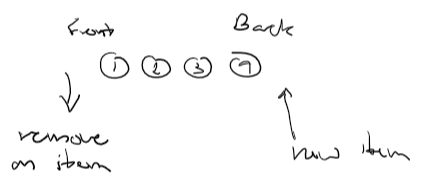
\includegraphics[width=.6\linewidth]{resources/queue.png}
\end{center}

\subsection{Divide-and-conquer algorithms: Binary Search}
\begin{itemize}
  \item A \bld{search algorithm} finds a target in a list.
  \item \bld{Binary Search} is an efficient algorithm to search for a target item in a \itl{sorted list}.
\end{itemize}
{\large Pseudo-code for recursive binary search:}
\begin{lstlisting}
RecBinSearch(low, high, A, x)

If(low = high AND a[low] = x), Return(low)
If(low = high AND a[low] != x), Return(-1)

mid := floor((low + high)/2)

If(x <= a[mid]), then high := mid
If(x > a[mid]), then low := mid+1

Return(RecBinSearch(low, high, A, x))
\end{lstlisting}

\subsection{Solving linear homogeneous recurrence relations}
Finding an explicit formula for a recursively defined sequence is called \itl{solving a recurrence relation}.
\subsubsection*{Linear Homogeneous Recurrence Relation}
A linear homogeneous recurrence relation of degree $k$ has the following form:
\[
  f_n = c_1f_{n-1} + c_2f_{n-2} + \cdots + c_kf_{n-k},
\]
where the $c_j$'s are constants that do not depend on $n$, and $c_k \neq 0$.
\begin{center}
  \begin{tabular}{ll}
    \multicolumn{2}{c}{Examples illustrating linear and non-linear recurrence relations} \\
    \hline
    $b_n = b_{n-1} + (b_{n-2} \cdot b_{n-3})$   & Non-linear                             \\
    $c_n = 3n \cdot c_{n-1}$                    & Non-linear                             \\
    $d_n = d_{n-1} + (d_{n-2})^2$               & Non-linear                             \\
    $f_n = 3f_{n-1} - 2f_{n-2} + f_{n-4} + n^2$ & Linear, degree 4. Non-homogeneous      \\
    $g_n = g_{n-1} + g_{n-3} + 1$               & Linear, degree 3. Non-homogeneous      \\
    $h_n = 2h_{n-1} - h_{n-2}$                  & Linear, degree 2. Homogeneous          \\
    $s_n = 2s_{n-1} = \sqrt{3}s_{n-5}$          & Linear, degree 5. Homogeneous
  \end{tabular}
\end{center}
The expression denoting the infinite set of solutions to a recurrence relation without initial values is called the \itl{general solution} to the recurrence relation.

\subsubsection*{Solutions to linear homogeneous recurrence relations}
If $g_n \tand h_n$ satisfy a linear homogeneous relation then so does $f_n = s\cdot g_n + t\cdot h_n$ for any real numbers $s \tand t$.

\subsubsection*{Using Initial Values to determine to unique solution to a recurrence relation}
Any ${\displaystyle f_n = c_1\left(\frac{1 + \sqrt{5}}{2}\right)^n + c_2\left(\frac{1 - \sqrt{5}}{2}\right)^n}$

\noindent Initial Values:
\begin{align*}
  n & = 0 & f_0 & = 0 = c_1\left(\frac{1 + \sqrt{5}}{2}\right)^0 + c_2\left(\frac{1 - \sqrt{5}}{2}\right)^0 = c_1 + c_2 = 0 \\
  n & = 1 & f_1 & = 1 = c_1\left(\frac{1 + \sqrt{5}}{2}\right) + c_2\left(\frac{1 - \sqrt{5}}{2}\right) = 1
\end{align*}
Then solving a two variable linear system of equations:
\[
  c_1 = \frac{1}{\sqrt{5}}, \qquad c_2 = -\frac{1}{\sqrt{5}}
\]
which then yields the specific solution of
\[
  f_n = \frac{1}{\sqrt{5}}\left(\frac{1 + \sqrt{5}}{2}\right)^n - \frac{1}{\sqrt{5}}\left(\frac{1 - \sqrt{5}}{2}\right)^n.
\]

\subsubsection*{General Steps}
\begin{enumerate}
  \item Use the recurrence relation to find the characteristic equation which will be $p(x) = 0$, where $p(x)$ is a degree $d$ polynomial.
  \item Find all solutions to the characteristic equation. Assume $p(x)$ has distinct roots $x_1, x_2, \ldots, x_d$.
  \item Every solution $f_n = (x_1)^n$ satisfies the recurrence relation. Therefore, any solution of the form $f_n = a_1(x_1)^n + \cdots + a_d(x_d)^n$ satisfies the recurrence relation.
  \item Each initial value gives a value of $f_n$ for a specific value for $n$. Plug the value for $n$ and $f_n$ into the above expression to get a linear equation with variables $a_1,a_2,\ldots,a_d$. There are $d$ linear equations (from the $d$ initial values) and $d$ variables.
  \item Solve for $a_1,a_2,\ldots,a_d$.
  \item Plug values for $a_1,a_2,\ldots,a_d$ back in to the expression for $f_n$ to get the closed form expression for $f_n$.
\end{enumerate}

\subsection{Solving linear non-homogeneous recurrence relations}
A \bld{non-homogeneous linear recurrence relation} is a linear recurrence relation with additional terms that are either a constant or a function of $n$. The recurrence relations below are all examples of homogeneous linear recurrence relations.
\begin{align*}
  f_n & = 3f_{n-1} + 10f_{n-2} + 2   \\
  f_n & = 3f_{n-1} + 10f_{n-2} + 24n \\
  f_n & = 3f_{n-1} + 10f_{n-2} + 3n
\end{align*}
The \bld{associated homogeneous recurrence relation} is the recurrence relation with the additional non-homogeneous terms dropped. For example the associated homogeneous recurrence relation for all of the recurrence relations give above is $f_n = 3f_{n-1} + 10f_{n-2}$.

\subsubsection*{Particular and homogeneous solutions}
The solution to a non-homogeneous linear recurrence relation is the sum of two parts: a \itl{homogeneous solution} plus a \itl{particular solution}. If the sequence is $\{f_n\}$, then the homogeneous solution is denoted by $f_n^{(h)}$ and the particular solution is denoted by $f_n^{(p)}$.
\begin{itemize}
  \item The homogeneous solution $f_n^{(h)}$ is the general solution to the associated homogeneous recurrence relation.
  \item The method for finding the particular solution $f_n^{(p)}$ is to guess the form of the particular solution and then check the guess.
\end{itemize}

\subsubsection*{Summary of all the steps}
\begin{enumerate}
  \item Find the homogeneous part of the solution which is the general solution to the associated homogeneous recurrence relation.
  \item Guess the correct form for the particular solution.
  \item Verify the guess by solving for constants so that the guess satisfies the recurrence relation for all $n$.
  \item Add the homogeneous and particular solutions to get the general solution.
  \item For a degree $d$ linear recurrence relation, there must be $d$ initial values to specify the sequence. Each initial value gives a value for $f_n$ for a specific value for $n$. Plug the values for $n$ and $f_n$ into the general solution to get a linear equation with variables $a_1,a_2,\ldots,a_d$. There are $d$ linear equations (from the $d$ initial values) and $d$ variables.
  \item Solve for $a_1,a_2,\ldots,a_d$.
  \item Plug values for $a_1,a_2,\ldots,a_d$ back in to the general solution for $f_n$ to get the final closed form expression for $f_n$.
\end{enumerate}

\subsection{Divide-and-conquer recurrence relations}
\subsubsection*{Deriving solutions to divide-and-conquer recurrence relations}
Many recurrence relations that describe the time complexity of divide-and-conquer algorithms have the form
\[
  T(n) = aT(n/b) + \Theta(n^d).
\]

\subsubsection*{Expressing the formula as a geometric sum}
The explicit formula for $T(n)$ can be generalized for a recurrence relation of the form $T(n) = aT(n/b) + n^d$ which has an explicit formula
\[
  T(n) = n^d \cdot \sum_{j=0}^{L}\left(\frac{a}{b^d}\right)^j~~\twhere L = \log_b n
\]
The expression for $n^d$ times the sum of terms in a geometric sequence of the form $1 + r + r^2 + \cdots + r^L$, where the ratio $r = a/b^d$. The formula for the sum of a geometric sequence is
\[
  1 + r + r^2 + \cdots + r^L = \sum_{j=0}^{L} r^j = \frac{r^{L+1}-1}{r-1}
\]
The asymptotic growth rate of $T(n)$ depends on whether the ratio $r$ is less than, greater than, or equal to 1.

\subsubsection*{The Master Theorem}
if $T(n) = aT(n/b) + \Theta(n^d)$ for constants $a>0,~b>1,\tand d \geq 0$, then
\begin{itemize}
  \item If $(a/b^d) < 1$, then $T(n) = \Theta(n^d)$
  \item If $(a/b^d) = 1$, then $T(n) = \Theta(n^d \log n)$
  \item If $(a/b^d) > 1$, then $T(n) = \Theta(n^{\log_b a})$
\end{itemize}
\section{Integer Properties}
\subsection{The Division Algorithm}
In \bld{integer division}, the input and output values must always be integers. For example, when 9 is divided by 4, the answer is 2 with a remainder of 1, instead of 2.25.

\subsubsection*{Divides}
Let $x \tand y$ be two integers. Then $x$ \itl{divides} $y$, $x \mid y$, if and only if $x \neq 0$ and there is an integer $k$ such that $y = kx$. If there is no such integer or if $x = 0$, then $x$ does not divide $y$, $x \nmid y$. If $x \mid y$, then $y$ is said to be a \itl{multiple} of $x$, and $x$ is a \itl{factor} or \itl{divisor} of $y$.

\subsubsection*{Theorem: Divisibility and linear combinations}
Let $x,y,\tand z$ be integers. If $x \mid y \tand x \mid z,~\tthen x \mid (sy+tz)$ for any integers $s \tand t$.
\begin{proof}
  Since $x \mid y$, then $y = kx$ for some integer $k$. Similarly, since $x \mid z$, then $z = jx$ for some integer $j$. A linear combination of $y \tand z$ can be expressed as:
  \[
    sy + tz = s(kx) + t(jx) = (sk + tj)x.
  \]
  For some integers $s \tand t$. Since $sy + tz$ is an integer multiple of $x$, then $x \mid (sy + tz)$.
\end{proof}

\subsubsection*{Quotients and remainders}
If $x \nmid y$, then there is s non-zero remainder when $x$ is divided into $y$. The \bld{Division Algorithm}, states that the result of the division and the remainder are unique.

\subsubsection*{Theorem: The Division Algorithm}
Let $n$ be an integer and let $d$ be a positive integer. Then, there are unique integers $q \tand r$, with $0 \leq r \leq d-1$, such that $n = qd + r$.

\subsubsection*{Integer division definitions}
In the Division Algorithm, $q$ is called the \bld{quotient} and $r$ is called the \bld{remainder}. The operations \bld{$\tdiv$} and \bld{$\tmod$} produce the quotient and the remainder as a function of $n \tand d$.
\begin{align*}
  q & = n \tdiv d \\
  r & = n \tmod d
\end{align*}
Here is some examples of computing $\tdiv \tand \tmod$:
\begin{align*}
  15 \tmod 6       & = 3 & -11 \tmod 4        & = 1  \\
  15 - 2 \cdot 6   & = 3 & -11 - (-3) \cdot 4 & = 1  \\ \\
  15 \tdiv 6       & = 2 & -11 \tdiv 4        & = -3 \\
  \frac{15 - 3}{2} & = 2 & \frac{-11 - 1}{4}  & = -3
\end{align*}

\subsection{Modular arithmetic}
Given a finite set of integers, we can define addition and multiplication on the elements in the set such that after every operation, we apply a modular function equal to the cardinality of the set.
\begin{itemize}
  \item \bld{addition mod $m$}
        \subitem the operation defined by adding two numbers and applying $\tmod m$ to the result
  \item \bld{multiplication mod $m$}
        \subitem the operation defined by multiplying two numbers and applying $\tmod m$ to the result
\end{itemize}
The set $\{0,1,2,\ldots,m-1\}$ along with addition and multiplication mod $m$ defines a closed mathematical system with $m$ elements called a \bld{ring}. The ring $\{0,1,2,\ldots,m-1\}$ with addition and multiplication mod $m$ is denoted by $\bb{Z}_m$.

\subsubsection*{Applications}
A common way to organize data is to maintain an array called a \bld{hash table} which is slightly larger than the number of data items to be stored. A bld{hash function} is used to map each data item to a location in the array. Modulus is used to keep the results from a hash function in the range of the hash table.

Computers use functions called bld{pseudo-random number generators} that produce numbers having many of the statistical properties of random numbers but are in fact deterministically generated. Modulus is used to keep these pseudo-random number generators in a certain range when used.

\subsubsection*{Congruence mod $m$}
Let $m \in \bb{Z} > 1$. Let $x \tand y$ be any two integers. Then bld{$x$ is congruent to $y \tmod m$} if $x \tmod m = y \tmod m$. The fact that $x$ is congruent to $y \tmod m$ is denoted
\[
  x \equiv y~(\tmod m).
\]

\subsubsection*{Theorem: Alternate characterization of congruence mod $m$}
Let $m \in \bb{Z} > 1$. Let $x \tand y$ be any two integers. Then $x \equiv y~(\tmod m)$ if and only if $m \mid (x-y)$.
\begin{proof}
  First suppose that $x \equiv y~(\tmod m)$. By definition $x tmod m = y \tmod m$. We define the variable $r$ to be the value of $x \tmod m = y \tmod m$. Therefore, $x = r + km$ for some integer $k$ and $y = r + jm$ for some integer $j$. Then
  \[
    x-y = (r+km)-(r+jm) = (k-j)m.
  \]
  Since $(k-j)$ is an integer, $m\mid (x-y)$. \\
  Now suppose that $m\mid (x-y)$. Then $(x-y) = tm$ for some integer $t$. Let $r$ be the value of $x \tmod m$. Then $x = r + km$ for some integer $k$. The integer $y$ can be expressed as
  \[
    y = x - (x-y) = (r+km)-tm = r + (k-t)m.
  \]
  Since $r$ is an integer in the range from $0$ to $m-1$, $r$ is the unique remainder when $y$ is divided by $m$. Therefore $r = y \tmod m = x \tmod m$, and by definition $x \equiv y~(\tmod m)$.
\end{proof}

\subsubsection*{Precedence of the mod operation}
\begin{align*}
  6 + 2 \tmod y = 6 + (2 \tmod 7)         & = 8 \\
  6 \cdot 2 \tmod 7 = (6 \cdot 2) \tmod 7 & = 5 \\
\end{align*}
However, in general it is best to just use parentheses in order to clarify which operations should be performed first.

\subsubsection*{Theorem: Computing arithmetic operations mod $m$}
Let $m$ be an integer larger than 1. Let $x \tand y$ be any integers. Then
\begin{align*}
  [(x \tmod m) + (y \tmod m)] \tmod m & = [x + y] \tmod m \\
  [(x \tmod m)(y \tmod m)] \tmod m    & = [x + y] \tmod m
\end{align*}

\subsection{Prime factorizations}
A number $p$ is \bld{prime} if it is an integer greater than $1$ and its only factors are $1 \tand p$. A positive integer is \bld{composite} if it has a factor other than 1 or itself. Every integer greater than 1 is either prime of composite. Every positive integer greater than one can be expressed as a product of primes called its \bld{prime factorization}. Moreover, the prime factorization is unique up to ordering of the factors.

\subsubsection*{Theorem: The Fundamental Theorem of Arithmetic}
Every positive integer other than 1 can be expressed uniquely as a product of prime numbers where the primes factors are written in non-decreasing order.

\begin{align*}
  \text{Examples of prime factorizations} & ~\text{in non-decreasing order} \\
  112                                     & = 2^4\cdot 7                    \\
  612                                     & = 2^2 \cdot 3^3 \cdot 17        \\
  243                                     & = 3^5                           \\
  17                                      & = 17
\end{align*}

\subsubsection*{Greater common divisors and least common multiples}
\begin{itemize}
  \item The \bld{greatest common divisor (gcd)} of integers $x \tand y$ that are not both zero is the largest integer that is a factor of both $x \tand y$.
  \item The \bld{least common multiples (lcm)} of non-zero integers $x \tand y$ is the smallest positive integer that is an integer multiple of both $x \tand y$.
\end{itemize}
Two numbers are \bld{relatively prime} if their greatest common divisor is 1.

\subsubsection*{Theorem: GCD and LCM from prime factorizations}
Let $x \tand y$ be two positive integers with prime factorizations expressed using a common set of primes as:
\begin{align*}
  x & = p_1^{\alpha_1} \cdot p_2^{\alpha_2} \cdots p_r^{\alpha_r} \\
  y & = p_1^{\beta_1} \cdot p_2^{\beta_2} \cdots p_r^{\beta_r}
\end{align*}
The $p_i$'s are all distinct prime numbers. The exponents $\alpha_i$'s and $\beta_i$'s are non-negative integers. Then:
\begin{itemize}
  \item $x \mid y$ if and only if $\alpha_i \leq \beta_i$ for all $1 \leq i \leq r$
  \item $\gcd(x,y) = p_1^{\min(\alpha_1,\beta_1)} \cdot p_2^{\min(\alpha_2,\beta_2)} \cdots p_r^{\min(\alpha_r,\beta_r)}$
  \item $\lcm(x,y) = p_1^{\max(\alpha_1,\beta_1)} \cdot p_2^{\max(\alpha_2,\beta_2)} \cdots p_r^{\max(\alpha_r,\beta_r)}$
\end{itemize}

\subsection{Factoring and primality testing}
A \bld{brute force algorithm} solves a problem by exhaustively searching all positive solutions without using an understanding of the mathematical structure in the problem to eliminate steps.

\subsubsection*{Theorem: Small Factors}
If $N$ is a composite number, then $N$ has a factor greater than 1 and at most $\sqrt{N}$

\subsubsection*{Theorem: Infinite number of primes}
There are an infinite number of primes.
\begin{proof}
  Suppose that there are a finite number of primes. Since there are only a finite number, they can be listed:
  \[
    p_1,p_2,\ldots,p_k
  \]
  Take the product of all the primes and add 1. Call the resulting number $N$:
  \[
    N = (p_1 \cdot p_2 \cdots p_k) + 1
  \]
  The number $N$ is larger than all of the primes numbers that were listed, so it must not be prime. Since $N$ is a composite number, it is the product of at least two primes by the Fundamental Theorem of Arithmetic. There $N$ is divisible by some prime $p_j$. Let
  \[
    \frac{N}{p_j} = \frac{(p_1 \cdot p_2 \cdots p_k)}{p_j} + \frac{1}{p_j}
  \]
  Note that $p_j$ is one of the prime factors in $(p_1 \cdot p_2 \cdots p_k)$, so $(p_1 \cdot p_2 \cdots p_k)/p_j$ is an integer. However, $1/p_j$ is not an integer. Since $N/p_j$ is the sum of two terms, one of which is an integer and the other of which is not an integer, then $N/p_j$ is not an integer. This contradicts the fact that $p_j$ evenly divides $N$.
\end{proof}

\subsubsection*{The Prime Number Theorem}
Let $\pi(x)$ be the number of prime numbers in the range from 2 through $x$. Then
\[
  \lim_{x \rightarrow \infty} \frac{\pi(x)}{x/\ln x} = 1.
\]
Another way to interpret the Prime Number Theorem is that if a random number is selected from the range 2 to $x$, then the likelihood that the selected number is prime is roughly $1/\ln x$.

\subsection{Greatest common factor divisor and Euclid's algorithm}
There is an efficient way to compute the gcd of two numbers without finding their prime factorizations. The algorithm presented in this subsection is in wide use today and is attributed to the Greek mathematician Euclid who lived around 300 B.C. The basis of the algorithm is the following theorem:

\subsubsection*{GCD Theorem}
Let $x \tand y$ be two positive integers. Then $\gcd(x,y) = \gcd(y \tmod x, x)$.

\subsubsection*{Euclid's Algorithm for finding the greatest common divisor}
\begin{lstlisting}
Input: Two positive integers, x and y.
Output: gcd(x, y)

If(y < x)
  Swap x and y.
r := y mod x

While(r != 0)
  y := x
  x := r
  r := y mod x
End-While

Return(x)
\end{lstlisting}
Sample execution of Euclid's algorithm for $\gcd(675,210)$:
\begin{center}
  \begin{tabular}{cccccc}
    $675$ & $210$ & $675 \tmod 210$                                                  \\
          & $210$ & $45$            & $210 \tmod 45$                                 \\
          &       & $45$            & $30$           & $45 \tmod 30$                 \\
          &       &                 & $30$           & $15$          & $30 \tmod 15$ \\
          &       &                 &                & $\bld{15}$    & $0$           \\
  \end{tabular}
\end{center}
The last non-zero number was $15$, so $\gcd(675,210) = 15$.

\subsubsection*{Expressing $\gcd(x,y)$ as a linear combination of $x$ and $y$}
Let $x \tand y$ be integers, then there are integers $s \tand t$ such that
\[
  \gcd(x,y) = sx + ty.
\]
The values for $s \tand t$ in the theorem above can be found by a series of substitutions using the equation from each iteration. The algorithm used to find the coefficient, $s \tand t$, such that $\gcd(x,y) = sx + ty$, is called the \bld{Extended Euclidean Algorithm}.

\subsubsection*{The Extended Euclidean Algorithm}
\[
  \begin{array}{lllll}
        &     & y           & x           & r                                \\
    675 & 210 & 45          & 30          & 15                               \\
        &     &             &             & r = y \tmod x                    \\
        &     &             &             & r = y - (y \tdiv x) \cdot x      \\
        &     &             &             & 15 = 45 - (45 \tdiv 30) \cdot 30 \\
        &     &             &             & \mathbf{15 = 45 - 1 \cdot 30}    \\
        &     &             & 30          & = 210 - (210 \tdiv 45) \cdot 45  \\
        &     &             & \mathbf{30} & \mathbf{= 210 - 4 \cdot 45}      \\
        &     & 45          & =           & 675 - (675 \tdiv 210) \cdot 210  \\
        &     & \mathbf{45} & \mathbf{=}  & \mathbf{675 - 3 \cdot 210}
  \end{array}
\]
We can use the bolded equations to solve for $15 = c \cdot 210 + d \cdot 675$.
\begin{align*}
  15 & = 45 - 30                           \\
     & = 45 - (210 - 4 \cdot 45)           \\
     & = 5 \cdot 45 - 210                  \\
     & = 5 \cdot (675 - 3 \cdot 210) - 210 \\
     & = 5 \cdot 675 - 16 \cdot 210
\end{align*}
Now we have the full answer and expansion for $\gcd(675,210)$.
\[
  \gcd(675,210) = 15 = 5 \cdot 675 - 16 \cdot 210.
\]

\subsubsection*{The Multiplicative Inverse mod $n$}
A \bld{multiplicative inverse mod $n$}, or just \bld{inverse mod $n$}, of an integer $x$, is an integer $s \in \{1,2,\ldots,n-1\}$ such that $sx \tmod n = 1$.

For example, 3 is an inverse of 7 $\tmod 10$ because $3 \cdot 7 \tmod 10 = 1$. The number 7 is an inverse of 5 $\tmod 17$ because $7 \cdot 5 \tmod 17 = 1$. It is possible for a number to be its own multiplicative inverse mod $n$. For example, $7$ is the inverse of $7 \tmod 8$ because $7 \cdot 7 \tmod 8 = 1$.

Not every number has an inverse mod $n$. For example, 4 does not have an inverse mod $6$. The condition is that $x$ has an inverse $\tmod n$ if and only if $x \tand n$ are relatively prime.

The Extended Euclidean Algorithm can be used to find the multiplicative inverse of $x \tmod n$ when is exists.
\begin{itemize}
  \item If $\gcd(x, n) \neq 1$, then $x$ does not have a multiplicative inverse $\tmod n$.
  \item If $x \tand n$ are relatively prime, then the Extended Euclidean Algorithm finds integers $s \tand t$ such that $1 = sx + tn$.
  \item $sx - 1 = -tn$. Therefore, $(sx \tmod n) = (1 \tmod n)$. If $A - B$ is a multiple of $n$ then $(A \tmod n) = (B \tmod n)$.
  \item $(s \tmod n)$ is the unique multiplicative inverse of $x$ in $\{0, 1, \ldots, n-1\}$.
\end{itemize}
For example, suppose that Euclid's Algorithm returns
\[
  \gcd(31, 43) = 1 = 13 \cdot 34 - 18 \cdot 31
\]
The coefficient of 31 is -18. Therefore, the multiplicative inverse of $31 \tmod 43$ is $(-18 \tmod 43) = 25$.

\subsection{Number representation}
A digit in binary is called a \bld{bit}. In binary notation, each place value is a power of 2. Numbers represented in \bld{base} $b$ require $b$ distinct symbols and each place value is a power of $b$.

\subsubsection*{Theorem: Number representation}
For an integer $b>1$. Every positive integer $n$ can be expressed uniquely as
\[
  n = a_k \cdot b^k + a_{k-1} \cdot b^{k-1} + \cdots + a_1 \cdot b^1 + a_0 \cdot b^0,
\]
where $k$ is a non-negative integer, and each $a_i$ is an integer in the range from $0 \tto b-1$, and $a_k \neq 0$.
The representation of $n~\text{base}~b$ is called the \bld{base $b$ expansion of $n$} and is denoted by $(a_ka_{k-1}\ldots a_1a_0)_b$.

\subsubsection*{Hexadecimal Numbers}
In \bld{hexadecimal} notation (or \bld{hex} for short), numbers are represented in base 16. Typically, the set of symbol, in order of value, is
\[
  \{0,1,2,3,4,5,6,7,8,9,A,B,C,D,E,F\}.
\]
Additionally, here are the first 15 hexadecimal digits and correspond encodings in decimal and binary.
\[
  \begin{array}{lccccccccc}
    \text{Hex}     & 0    & 1    & 2    & 3    & 4    & 5    & 6    & 7    \\
    \text{Decimal} & 0    & 1    & 2    & 3    & 4    & 5    & 6    & 7    \\
    \text{Binary}  & 0    & 1    & 10   & 11   & 100  & 101  & 110  & 111  \\ \\
    \text{Hex}     & 8    & 9    & A    & B    & C    & D    & E    & F    \\
    \text{Decimal} & 8    & 9    & 10   & 11   & 12   & 13   & 14   & 15   \\
    \text{Binary}  & 1000 & 1001 & 1010 & 1011 & 1100 & 1101 & 1110 & 1111
  \end{array}
\]
Since both hexadecimal and binary are powers of 2, there is an easy way to translate between the binary expansion and the hexadecimal expansion of a number. Groups of 4 binary digits can be directly translated into hexadecimal digits. Here is an example
\[
  \begin{array}{ccccc}
    1 & 1101 & 0101 & 1110 & 1000 \\
    1 & D    & 5    & E    & 8
  \end{array} \qquad 1,1101,0101,1110,1000_2 = 1D5E8_{16}
\]
Hexadecimal notation is particularly useful in computer science because each hexadecimal digit can be used to represent a 4-bit binary number. A byte, which consists of 8 bits, can be represented by a 2-digit hexadecimal number. Two hexadecimal digits is easier for a human to recognize and remember than 8 bits.

\subsubsection*{Converting decimal numbers to base $b$}
\[
  \left[\text{Base $b$ expansion of $(n \tdiv b)$}\right]\left[n \tmod b\right]
\]
Here is an example of $1161_{10}$ converted to base 7:
\[
  \begin{array}{ccccc}
     &            &             & \ulcorner    & 1161         \\
     &            &             & 1161 \tdiv 7 & 1161 \tmod 7 \\
     &            & \ulcorner   & 165          & 6            \\
     &            & 165 \tdiv 7 & 165 \tmod 7  & |            \\
     & \ulcorner  & 23          & 4            & |            \\
     & 23 \tdiv 7 & 23 \tmod 7  & |            & |            \\
     & 3          & 2           & |            & |            \\
     & 3          & 2           & 4            & 6            \\
  \end{array}
\]

\subsubsection*{The number of digits required to represent a number}
\[
  n = (\underbrace{[b-1][b-1]\ldots[b-1]}_{k \text{digits}})_b = (1\underbrace{00\ldots 0}_{k 0's})_b -1 = b^k - 1
\]
The number of digits required to expressed the base $b$ expansion of a positive integer $n$ is $\left\lceil \log_b (n+1) \right\rceil$. For example, the number of digits required to express the base 2 expansion of 13 is:
\[
  \left\lceil\log_2 (13 + 1)\right\rceil = \left\lceil \log_2(14)\right\rceil = \left\lceil 3.8 \right\rceil = 4.
\]

\subsection{Fast exponentiation}
Computing a power of $x$ by repeated multiplication by $x$
\[
  p:=x \xrightarrow{p:=p*x} p = x^2 \xrightarrow{p:=p*x} p = x^3 \xrightarrow{p:=p*x} p=x^4 \cdots
\]
Computing a power of $x$ by repeated squaring
\[
  p:=x \xrightarrow{p:=p*p} p=x^2 \xrightarrow{p:=p*p} p=x^4 \xrightarrow{p:=p*p} p=x^8 \cdots
\]
In order to compute $x^y$, examine the binary expansion of y:
\[
  y = a_k \cdot 2^k + a_{k-1} \cdot 2^{k-1} + \cdots + a_1 \cdot 2^1 + a_0 \cdot 2^0
\]
We can use this expanded form of $y$ to represent $x$ as a sum of perfect squares
\[
  x^y = x^{a_k \cdot 2^k + a_{k-1} \cdot 2^{k-1} + \cdots + a_1 \cdot 2^1 + a_0 \cdot 2^0} = x^{a_{k} \cdot 2^{k}} \cdot x^{a_{k-1} \cdot 2^{k-1}} \cdots x^{a_{1} \cdot 2^{1}} \cdot x^{a_{0} \cdot 2^{0}}
\]
Each coefficient $a_j$ is either $0 \tor 1$. If $a_j = 0$ for some $j$, then
\[
  x^{a_j \cdot 2^j} = x^0 = 1
\]
and the corresponding factor can be omitted from the product. Here is an example, computing $7^{11}$.
\begin{align*}
  7^{11} & = 7^{[(1 \cdot 2^3) + (0 \cdot 2^2) + (1 \cdot 2^1) + (1 \cdot 2^0)]}               \\
         & = 7^{(1 \cdot 8)} \cdot 7^{(0 \cdot 4)} \cdot 7^{(1 \cdot 2)} \cdot 7^{(1 \cdot 7)} \\
         & = 7^8 \cdot 1 \cdot 7^2 \cdot 7^1                                                   \\
  7^11   & = 5,764,801 \cdot 49 \cdot 7                                                        \\
         & = 1,977,326,743
\end{align*}

\subsubsection*{An iterative algorithm for fast exponentiation}
\begin{lstlisting}
Input: Positive integers x and y.
Output: x^y

p := 1  // p holds the partial result
s := x  // s holds the current x^{2^j}
r := y  // r is used to compute the binary expansion of y

while(r > 0)
  if(r mod 2 = 1)
    p := p * s
  s := s * s
  r := r div 2
End-While

Return(p)
\end{lstlisting}

\subsubsection*{An iterative algorithm for fast modular exponentiation}
\begin{lstlisting}
Input: Positive integers x, y and n.
Output: x^y mod n

p := 1  // p holds the partial result
s := x  // s holds the current x^{2^j}
r := y  // r is used to compute the binary expansion of y

while(r > 0)
  if(r mod 2 = 1)
    p := p * s mod n
  s := s * s mod n
  r := r div 2
End-While

Return(p)
\end{lstlisting}

\subsection{Introduction to cryptography}
\bld{Cryptography} is the science of protecting and authenticating data and communication. Cryptography is ubiquitous in the electronic age in which sensitive information such as credit card numbers and passwords are sent over the internet on a daily basis.

A cryptosystem is a system by which a \bld{sender} sends a message to a \bld{receiver}. The sender \bld{encrypts} the message so that if an eavesdropper learns the transmitted message, they will be unable to recover the original message. The unencrypted message is called \bld{plaintext} and the encrypted message is called the \bld{ciphertext}. The receiver must have a \bld{secret key} that allows him to \bld{decrypt} the ciphertext to obtain the original plaintext.

\subsubsection*{Sending an Encrypted Text Message via a Secret Key}
\begin{enumerate}
  \item Alice wants to send the message "MEET AT DAWN" to Bob. Alice converts the text message to the number 130505202701292704012314.
  \item Alice encrypts the numerical message with her copy of the secret key.
  \item Alice sends encrypted message to Bob. Eve cannot read the encrypted message without the secret key.
  \item Bob decrypts the encrypted message using the secret key to get 130505202701292704012314 which he then converts to "MEET AT DAWN".
\end{enumerate}

\subsubsection*{Encryption and Decryption Functions}
Consider a simple cryptosystem in which the set of all possible plaintexts come from $\bb{Z}_N$ for some integer $N$. Alice and Bob share a secret number $k \in \bb{Z}_N$. The security of their encryption scheme rests on the assumption that no one besides them knows the number $k$. To encrypt a plaintext $m \in \bb{Z}_n$, Alice computes:
\[
  c = (m + k) \tmod N \qquad \qquad \text{(encryption)}
\]
Alice sends the ciphertext $c$ to Bob. When Bob receives the ciphertext $c$, he decrypts $c$ as follows:
\[
  m = (c - k) \tmod N \qquad \qquad \text{(decryption)}
\]
The simple encryption scheme presented here is an example of symmetric key cryptography. In a \bld{symmetric key cryptosystem}, Alice and Bob must meet in advance to decide on the value of a shared secret key.

\subsubsection*{Simple encryption scheme requirements}
\begin{itemize}
  \item If $m \neq m' \tand m,~m' \in \bb{Z}_N \tthen (m+k) \tmod N \neq (m'+k) \tmod N$ (no two distinct plaintexts map to same ciphertext).
  \item If $m \in \bb{Z}_N \tthen (((m+k) \tmod N)-k) \tmod N = m$ (decryption scheme is inverse of encryption scheme).
\end{itemize}
However, this encryption method is not terribly secure, and is not used in real world conditions because better methods exist.

\subsection{The RSA cryptosystem}
In \bld{public key cryptography}, Bob has an \bld{encryption key} that he provides \itl{publicly} so that anyone can use it to send him an encrypted message. Bob holds a matching \bld{decryption key} that he keeps \itl{privately} to decrypt messages. While anyone can use the public key to encrypt a message, the security of the scheme depends on the fact that it is difficult to decrypt the message without having the matching private decryption key.
\begin{enumerate}
  \item Alice encrypts her message to Bob using the public key.
  \item Alice sends the encrypted message to Bob. Eve cannot read the encrypted message.
  \item Bob decrypts the message using his private key.
\end{enumerate}

\subsubsection*{Preparation of public and private keys in RSA}
\begin{enumerate}
  \item Bob selects two large prime numbers, $p \tand q$.
  \item Bob computes $N = pq \tand \phi = (p-1)(q-1)$.
  \item Bob finds an integer $e$ such that $\gcd(e, \phi) = 1$.
  \item Bob computes the multiplication inverse of $e \tmod \phi$: an integer $d$ such that $(ed \tmod \phi) = 1$.
  \item Public (encryption) key: $N \tand e$.
  \item Private (decryption) key: $d$.
\end{enumerate}
The RSA scheme requires that $m$, the message, is an integer in $\bb{Z}_N$ and is not a multiple of $p \tor q$. Since $p \tand q$ are primes with hundreds of digits, it is extremely unlikely that $m$ is a multiple of primes $p \tor q$. Alice encrypts her plaintext using $e \tand N$ to produce ciphertext $c$ as follows:
\[
  c = m^e \tmod N \qquad \qquad \text{(encryption)}
\]
Alice transmits $c$ to Bob. Bob decrypts the ciphertext using $d$ to recover $m$ from $c$:
\[
  m = c^d \tmod N \qquad \qquad \text{(decryption)}
\]

\subsubsection*{Number theoretic fact to establish correctness of RSA}
Let $p \tand q$ be prime numbers and $pq = N$. Suppose that $m \in \bb{Z}_n \tand \gcd(m,N) = 1$. Then $m^{(p-1)(q-1)} \tmod N = 1$.
\section{Introduction to Counting}
\subsection{Sum and Product Rules}

The two most basic rules of counting are the sum and product rule. The \bld{product rule} provides a way to count sequences.

\subsubsection*{Theorem: The Product Rule}
Let $A_1,A_2,\ldots,A_n$ be finite sets. Then,
\[
  | A_1 \times A_2 \times \cdots \times A_n | = |A_1| \cdot |A_2| \cdots |A_n|
\]

\subsubsection*{Counting Strings}
If $\Sigma$ is a set of characters (called an \bld{alphabet}) then $\Sigma^n$ is the set of all string of length $n$ whose characters come from the set $\Sigma$. The product rule can be applied directly to determine the number of strings of a given length over a finite alphabet:
\[
  |\Sigma^n| = |\underbrace{\Sigma \times \Sigma \times \cdots \Sigma}_{\text{$n$ times}}| = \underbrace{|\Sigma| \cdot |\Sigma| \cdots |\Sigma|}_{\text{$n$ times}} = |\Sigma|^n
\]

\subsubsection*{Theorem: The Sum Rule}
Consider $n$ sets, $A_1, A_2, \ldots, A_n$. If the sets are pairwise disjoint, meaning that $A_i \cap A_j = \emptyset \tfor i \neq i$, then
\[
  |A_1 \cup A_2 \cup \cdots \cup A_n| = |A_1| + |A_2| + \cdots + |A_n|
\]

\subsection{The Bijection Rules}
One way to approach difficult counting problems is to show that the cardinality of the set to be counted is equal to the cardinality of a set that is easy to count. The \bld{bijection rule} says that if there is a bijection from one set to another then the two sets have the same cardinality.

A function $f$ from a set $S$ to a set $T$ is called a bijection if and only if $f$ has a well-defined \itl{inverse}, $f^{-1}$.

\subsubsection*{The Bijection Rule}
Let $S \tand T$ be two finite sets. If there is a bijection from $S \tto T$, then $|S|=|T|$

\subsubsection*{The k-to-1 Rule}
Let $X \tand Y$ be finite sets. The function $f: X \rightarrow Y$ is a \bld{k-to-1 correspondence} if for every $y \in Y$, there are exactly $k$ difference $x \in x$ such that $f(x) = y$.

Suppose there is a k-to-1 correspondence from a finite set $A$ to a finite set $B$. Then
\[
  |B| = \frac{|A|}{k}.
\]

\subsection{The generalized product rule}
The \bld{generalized product rule} says that in selecting an item from a set, if the number of choices at each step does not depend on previous choices made, then the number of items in the set is a product of the number of choices in each step.

\subsubsection*{Generalized Product Rule}
Consider a set $S$ of sequences of $k$ items. Suppose there are:
\begin{itemize}
  \item $n_1$ choices for the first item.
  \item For every possible choice for the first item, there are $n_2$ choice for the second item.
  \item For every possible choice for the first and second items, there are $n_3$ choices for the third item.
  \item $\vdots$
  \item For every possible choice for the first $k-1$ items, there are $n_k$ choices for the $k$-th item.
\end{itemize}
Then $|S| = n_1 \cdot n_2 \cdots n_k$.

\subsection{Counting permutations}
An \bld{r-permutation} is a sequence of $r$ items with \bld{no repetitions}, all taken from the same set. In a sequence, order matters, so $(a,b,c)$ is different from $(b,a,c)$.

\subsubsection*{The number of $r$-permutations from a set with $n$ elements}
Let $r \tand n$ be positive integers with $r \leq n$. The number of $r$-permutations from a set with $n$ elements is denoted by $P(n,r)$:
\[
  P(n,r) = \frac{n!}{(n-r)!} = n(n-1)\cdots(n-r+1)
\]

\subsection{Counting subsets}
A subset of size $r$ is called an \bld{r-subset}. An $r$-subset is sometimes referred to as an \bld{r-combination}. In a subset, order does not matter, so $\{a,b,c\}$ is the same as $\{b,a,c\}$. The counting rules for sequences and subsets are commonly referred to as "\itl{permutations} and \itl{combinations}". The term "combination" is the context of counting is another word for "subset".

\subsubsection*{Counting Subsets: 'n choose r' notation}
The number of ways to select an $r$-subset from a set of size $n$ is:
\[
  \binom{n}{r} = \frac{n!}{r!(n-r)!}.
\]
$\binom{n}{r}$ is read as "$n$ choose $r$". The notation $C(n,r)$ is sometimes used for $\binom{n}{r}$.

We can calculated an expression for $\binom{n}{n-r}$ by replacing $r$ with $n-r$ in the expression for $\binom{n}{r}$.
\[
  \binom{n}{n-r} = \frac{n!}{(n-r)!(n-(n-r))!} = \frac{n!}{(n-r!)r!} =
  \binom{n}{r}
\]
This is an \bld{identity} for $r$-subsets.

\subsection{Subset and permutation examples}

\subsubsection*{Two different cat selection problems: Subset vs. Permutations}
Consider two closely related counting problems:
\begin{enumerate}
  \item A family goes to the animal shelter to adopt 3 cats. The shelter has 20 different cats from which to select. How many ways are there for the family to their selection?
  \item Three different families go to the animal shelter to adopt a cat. Each family will select one cat. How many ways are there for the families to make their selection? (Note that which family gets which cat matters).
\end{enumerate}
In the first problem, the number is ways to make the selection is $\binom{20}{3}$ because the order in which the cats are selected is not important. The outcome is a 3-subset.

In the second problem, the specific cat selected by each family is important. Additionally, no cat can belong to two families. Thus, the answer is $P(20,3) = 20 \cdot 19 \cdot 18$. The outcome is a 3-permutation.

\subsection{Counting by complement}
\bld{Counting by complement} is a technique for counting the number of elements in a set $S$ that have a property by counting the total number of elements in $S$ and subtracting the number of elements in $S$ that do not have the property.
\[
  |P| = |S| - |\overline{P}|
\]
Suppose we want to count the number of people in a room with red hair. We know that there are 20 people in the room and exactly 12 of them do not have red hair. Then we can deduce that the number of people in the room with red hair is 20 - 12 = 8.

\subsection{Permutations with repetitions}
A \bld{permutation with repetition} is an ordering of a set of items in which some of the items may be identical to each other. To illustrate with a smaller example, there are $3! = 6$ permutations of the letters CAT, because the letters in CAT are all different. However, there are only 3 different ways to scramble the letters in DAD: ADD, DAD, DDA.

\subsubsection*{Formula for Counting Permutations with Repetition}
The number of distinct sequences with $n_1 1's, n_2's, \ldots, n_k k's$, where $n = n_1 + n_2 + \cdots + n_k$ is
\[
  \frac{n!}{n_1!n_2!\cdots n_k!}
\]
The formula for permutations with repetition is derived from repeated use of the formula for counting r-subsets:
\begin{align*}
    & \binom{n}{n_1} \binom{n-n_1}{n_2} \binom{n-n_1-n_2}{n_3} \cdots \binom{n-n_1-n_2-\cdots-n_{k-1}}{n_k}                                                                                                                                \\
  = & \frac{n!}{n_1!{\color{red}(n-n_1)!}} \cdot \frac{{\color{red}(n-n_1)!}}{n_2!{\color{blue}(n-n_1-n_2)!}} \cdot \frac{\color{blue}(n-n_1-n_2)!}{n_3!{\color{green}(n-n_1-n_2-n_3)!}} \cdots \frac{(n-n_1-n_2-\cdots-n_{k-1})!}{n_k!0!} \\
  = & \frac{n!}{n_1!n_2!\cdots n_k!}
\end{align*}

\subsection{Counting multisets}
A set is a collection of distinct items. A \bld{multiset} is a collection that can have multiple instances of the same kind of item. When $\{1,2,2,3\}$ is viewed as a set, the repetitions don't matter and $\{1,2,2,3\} = \{1,2,3\}$. However, when $\{1,2,2,3\}$ is viewed as a multiset, then the fact there are two occurrences of 2 is important, and $\{1,2,2,3\} \neq \{1,2,3\}$. Two multisets are equal if they have the same number of each type of element. For multisets, the order of elements still does not matter.

\subsubsection*{Rules for encoding a selection of $n$ objects from $m$ varieties}
\begin{center}
  \begin{tabular}{|c|c|}
    \hline
    Selections                                               & Code words                                     \\
    \hline
    $n=$ number of items to select                           & $n=$ number of 0's in code word                \\
    $m=$ number of varieties                                 & $m-1=$ number of 1's in code word              \\
    Number selected from the first variety                   & Number of 0's before the first 1               \\
    Number selected from the $i$-th variety, for $1 < i < m$ & Number of 0's between the $i$-1st and $i$-th 1 \\
    Number selected from the last variety                    & Number of 0's after the last 1                 \\
    \hline
  \end{tabular}
\end{center}
If the mapping of selections to code words is a bijection, then by the bijection rule, the number of distinct code words is equal to the number of distinct selections. If the number of objects to select is $n$, and the number of varieties of object is $m$, each code word has $n$ 0's and $m-1$ 1's, for a total of $n+m-1$ bits. The binary string of length $n+m-1$ with exactly $m-1$ 1's is
\[
  \binom{n+m-1}{m-1}
\]

\subsubsection*{Theorem: Counting Multisets}
The number of ways to select $n$ objects from a set of $m$ varieties is
\[
  \binom{n+m-1}{m-1},
\]
if there is no limitation on the number of each variety available and objects of the same variety are indistinguishable.

A set of identical items are called \bld{indistinguishable} because it is impossible to distinguish one of the item from another. A set of different or distinct items are called \bld{distinguishable} because it is possible to distinguish one of the items from the others.

\subsection{Assignment problems: Balls in bins}
\begin{center}
  \begin{tabular}{c|c|c|c}
                            & \bld{No restrictions}      & \bld{Max 1 ball per bin}   & \bld{Same \# of balls per bin}          \\
                            & (any positive $m$ and $n$) & ($m$ must be at least $n$) & ($m$ must evenly divide $n$)            \\
    \hline
    \bld{Indistinguishable} & $\binom{n+m-1}{m-1}$       & $\binom{m}{n}$             & 1                                       \\
    \bld{Distinguishable}   & $m^n$                      & $P(m,n)$                   & ${\displaystyle \frac{n!}{((n/m)!)^m}}$
  \end{tabular}
\end{center}

\subsection{Inclusion-exclusion principle}
The \bld{principle of inclusion-exclusion} is a technique for determining the cardinality of the union sets that uses the cardinality of each individual set as well as the cardinality of their intersections.

\subsubsection*{The inclusion-exclusion principle with two sets}
Let $A \tand B$ be two finite sets, then $|A \cup B| = |A| + |B| - |A \cap B|$

\subsubsection*{The inclusion-exclusion principle with three sets}
Let $A, B, \tand C$ be three finite sets, then
\[
  |A \cup B \cup C| = |A| + |B| + |C| - |A \cap B| - |B \cap C| - |A \cap C| + |A \cap B \cap C|
\]

\subsubsection*{The inclusion-exclusion principle with an arbitrary number of sets}
Let $A_1,A_2,\ldots,A_n$ be a set of $n$ finite sets.
\begin{align*}
  |A_1 \cup A_2 \cup \cdots \cup A_n| & = \sum_{j=1}^{n} |A_j|                                         \\
                                      & - \sum_{1 \leq j \leq k \leq n} |A_j \cap A_k|                 \\
                                      & + \sum_{1 \leq j \leq j \leq l \leq n} |A_j \cap A_k \cap A_l| \\
                                      & ~~\vdots                                                       \\
                                      & + (-1)^{n+1} |A_1 \cap A_2 \cap \cdots \cap A_n|
\end{align*}

\subsubsection*{The inclusion-exclusion principle and the sum rule}
A collection of sets is \bld{mutually disjoint} if the intersection of every pair of sets in the collection is empty. If we apply the principle of inclusion-exclusion to determine the union of a collection of mutually disjoint sets, then all the terms with the intersections are zero. Thus, for a collection of mutually disjoint sets, the cardinality of the union of the sets is just equal to the sum of the cardinality of each of the individual sets:
\[
  |A_1 \cup A_2 \cup \cdots \cup A_n| = |A_1| + |A_2| + \cdots + |A_n|.
\]
The equation above is a restatement of the sum rule which only applies when the sets are mutually disjoint.

\subsubsection*{Determining the Cardinality of a Union by Complement}
Counting by complement can be used to express the size of the union as:
\[
  |U| - |\overline{P_1 \cup P_2 \cup \cdots \cup P_n}| = |P_1 \cup P_3 \cup \cdots \cup P_n|
\]
\section{Advanced Counting}
\subsection{Generating permutations}
There are situations in which it is necessary to generate, not just count, all permutations of a set or subsets of a given size.

\subsubsection*{Lexicographic Order}
A well-defined order imposed on the n-tuples is useful to systematically generate all the elements in a set of n-tuples. Generating the n-tuples in the set from smallest to largest ensures that each n-tuple is generated exactly once.

\bld{Lexicographic order} is a way or ordering n-tuples in which two n-tuples are compared according to the first entry where they differ. An example of such ordering is the word in a dictionary.

\subsubsection*{Generating Permutations}
A \bld{permutation} of the set $\{1,2,\ldots,n\}$ is an ordered n-tuple in which each number in $\{1,2,\ldots,n\}$ appears exactly once. For example, $(2,5,1,4,3)$ is a permutation of the set $\{1,2,3,4,5\}$.

\subsubsection*{Generating r-subsets of a set}
Unlike sequences or n-tuples, the order in which the elements of a set or subset are written does not matter. Sets can be ordered lexicographically by first sorting the elements in increasing order and then comparing the two sets as if they were ordered sequences. For example, $\{2,3,11\} < \{2,5,6\}$, because the first element is the same in both sets but in the second element $3 < 5$.

\subsection{Binomial coefficients and combinatorial identities}
An \bld{identity} is a theorem stating that two mathematical expressions are equal.

\subsubsection*{Theorem: A Simple Combinatorial Identity}
For any non-negative integers $n \tand k \tsuchthat k \leq n$:
\[
  \binom{n}{k} = \binom{n}{n-k}
\]

A proof that makes use of counting principles is called a \bld{combinatorial proof}. Combinatorial proofs usually involve defining a set $S$ and counting the number of elements in $S$ to get a mathematical expression for the number of items in the set. Every combinatorial proof of an identity uses a bijection implicitly as part of the argument.

\subsubsection*{Theorem: The Binomial Theorem}
For any non-negative integer $n$ and any real numbers $a \tand b$:
\[
  (a + b)^n = \sum_{k=0}^{n} \binom{n}{k} a^{n-k}b^k = \sum_{k=0}^{n} \binom{n}{k} a^kb^{n-k}
\]
The coefficients $\binom{n}{k}$ are called binomial coefficients.

For the case $n = 5$, the Binomial Theorem says that
\begin{align*}
  (a+b)^5 & = \binom{5}{0}a^5 + \binom{5}{1}a^4b + \binom{5}{2}a^3b^2 + \binom{5}{3}a^2b^3 + \binom{5}{4}ab^4 + \binom{5}{5}b^5 \\
          & = a^5 + 5a^4b + 10a^3b^2 + 10a^2b^3 + 5ab^4 + b^5
\end{align*}

The Binomial Theorem can also be used to obtain combinatorial identities. For example, by plugging in $a=b=1$, the Binomial Theorem yields the identity below.
\[
  2^n = \sum_{k=0}^{n} \binom{n}{k}
\]

Similarly, by letting $a=-1 \tand b=1$, and requiring that $n$ be positive, the left hand side of the Binomial Theorem becomes 0. The right hand side of the Binomial Theorem becomes:
\[
  0 = \sum_{k=0}^{n}(-1)^k \binom{n}{k}
\]
In the expanded form,
\[
  \binom{n}{0} - \binom{n}{1} + \binom{n}{2} - \binom{n}{3} + \cdots + (-1)^n \binom{n}{n} = 0
\]

\subsubsection*{Pascal's Triangle}
The $17^{th}$ century French mathematician, Blaise Pascal, developed a triangular chart that contains all the number of the form $\binom{n}{k}$. The chart, now known as Pascal's Triangle, can be used to derive the value of a particular $\binom{n}{k}$. The $n^{th}$ row of Pascal's Triangle contains the $n+1$ binomial coefficients of the form $\binom{n}{k}$ as shown in the figure below.
\[
  \begin{array}{cccccccccc}
    n=0 &              &              &              &              & \binom{0}{0} &              &              &                             \\
    n=1 &              &              &              & \binom{1}{0} &              & \binom{1}{1} &              &                             \\
    n=2 &              &              & \binom{2}{0} &              & \binom{2}{1} &              & \binom{2}{2} &                             \\
    n=3 &              & \binom{3}{0} &              & \binom{3}{1} &              & \binom{3}{2} &              & \binom{3}{3}                \\
    n=4 & \binom{4}{0} &              & \binom{4}{1} &              & \binom{4}{2} &              & \binom{4}{3} &              & \binom{4}{4} \\
  \end{array}
\]

\subsubsection*{Theorem: Pascal's Identity}
For any positive $n \tand k \tsuchthat k < n$:
\[
  \binom{n}{k} = \binom{n-1}{k-1} + \binom{n-1}{k}
\]

\subsection{The pigeonhole principle}
The pigeonhole principle is a mathematical tool used to establish that repetitions are guaranteed to occur in certain sets and sequences. The \bld{pigeonhole principle} says that if $n+1$ pigeons are placed in $n$ boxes, then there must be at least one box with more than one pigeon. The diagram below shows 10 pigeons, represented as $P$, in 9 boxes.
\begin{center}
  \begin{tabular}{ccc}
    $P$ & $P$ & $P$   \\
    $P$ & $P$ & $P,P$ \\
    $P$ & $P$ & $P$
  \end{tabular}
\end{center}

\subsubsection*{Theorem: The Pigeonhole Principle}
If a function $f$ has a domain of size at least $n+1$ and a target of size at most $n$, where $n$ is a positive integer, then there are two elements in the domain that map to the same element in the target (i.e., the function is not one-to-one)

\subsubsection*{Theorem: The Generalized Pigeonhole Principle}
Consider a function whose domain has at least $n$ elements and whose target has $k$ elements, for $n \tand k$ positive integers. Then there is an element $y$ in the target such that $f$ maps at least $\lceil n/k \rceil$ elements in the domain to $y$.

\subsubsection*{Theorem: Converse of the Generalized Pigeonhole Principle}
Suppose that a function $f$ maps a set of $n$ elements to a target with $k$ elements, where $n \tand k$ are positive integers. In order to guarantee that there is an element $y$ in the target to which $f$ maps to at least $b$ elements from the domain, then $n$ must be at least $k(b-1)+1$.

\subsection{Generating functions}
Generating functions are a powerful tool that can be used to solve a variety of problems related to counting and recurrence relations. A \bld{generating function} is a way of representing a sequence of number as a n algebraic function in which each term in the sequence is a coefficient of an $x^j$ term in the function. The advantage of representing sequences algebraically is that there are many techniques from algebra that can be used to manipulate functions which then leads to insight about the sequences they represent.

The sequence $f_0,f_1,f_2,f_3,\ldots$ is represented by the generating function
\[
  F(x) = f_0 + f_1x + f_2x^2 + f_3x^3 + \cdots
\]

The numbers in the sequence are the coefficients of the terms in $F(x)$. For the sequence $1,1,1,1,\ldots$ is represented by the generating function
\[
  H(x) = 1 + x + x^2 + x^3 + \cdots
\]
When $|x|<1$ for $H(x)$ the sum is finite and has a closed form of
\[
  H(x) = \sum_{j=0}^{\infty} x^j = \frac{1}{1-x}
\]
Additionally, for the partial sum up to $x^k$,
\[
  \sum_{j=0}^{k} x^j = \frac{1-x^k}{1-x}
\]

\subsubsection*{Using Generating Functions for Counting}
One of the primary uses for generating functions is to help solve counting problems. In general, $f_j$ is the number of way to select a subset of $j$ objects.

Consider the situation in which there is a set of two apples and one banana. The apples are indistinguishable, so selecting one apple is the same as selecting the other.
\begin{center}
  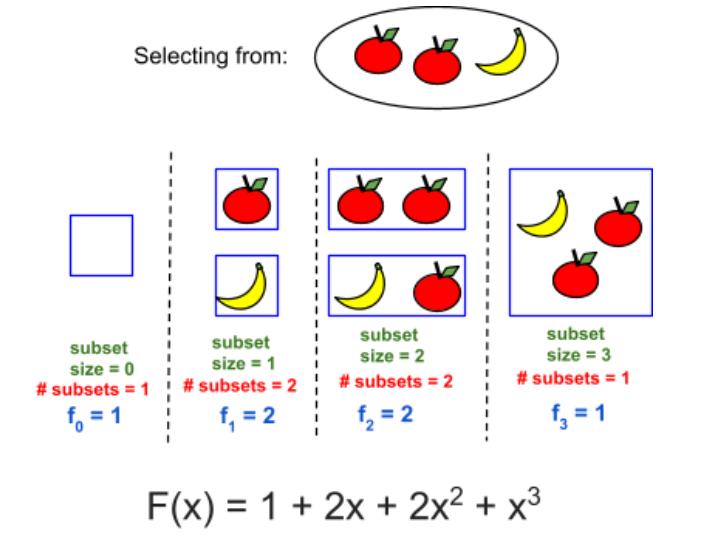
\includegraphics[width=.6\linewidth]{resources/11_two_apple_one_banana.png}
\end{center}

If the set from which the subsets are selected is an infinite set, then the resulting sequence is also infinite.

\subsubsection*{Summary of Generating Functions}
\begin{center}
  \begin{tabular}{|c|c|c|}
    \hline
    Description                                                  & Long Form                            & Short Form                               \\
    \hline
    Infinite supply of one kind of item                          & $1 + x + x^2 + x^3 + \cdots$         & ${\displaystyle \frac{1}{1-x}}$          \\
    \hline
    Selecting from a set of $n$ identical items                  & $1 + x + x^2 + x^3 + \cdots + x^n$   & ${\displaystyle \frac{1-x^{n-1}}{1-x}}$. \\
    \hline
    Infinite supple of identical items grouped in batches of $k$ & $1 + x^k + x^{2k} + x^{3k} + \cdots$ & ${\displaystyle \frac{1}{1-x^k}}$        \\
    \hline
    Infinite supple of 2 different kinds of items                & $1 + 2x + 3x^2 + 4x^3 + \cdots$      & ${\displaystyle \frac{1}{(1-x)^2}}$      \\
    \hline
  \end{tabular}
\end{center}

\subsubsection*{Products of Generating Functions}
Generating functions become very useful when different sets of objects are combined together into larger sets.

For example, if we are selecting subsets of apples from a set of 3 apples, the generating function is $A(x) = 1 + x + x^2 + x^3$, and if we are selecting bananas from a set of 2 bananas, the generating function is $B(x) = 1 + x + x^2$. Now suppose we pool the three apples and two bananas into a set of five pieces of fruit and ask 'how many ways can one select a set of fruit from the collection of five pieces of fruit?'

The power of generating functions is illustrated in the fact that if we take the product of $A(x)$, the generating function for apples, and $B(x)$, the generating function for bananas, to get $A(x)B(x)$, then the resulting product is the generating function for the pooled set of five pieces.
\[
  A(x)B(x) = (1 + x + x^2 + x^3)(1 + x + x^2) = 1 + 2x + 3x^2 + 3x^3 + 2x^4 + x^5
\]
Note that the rule of multiplying generating function only works when the two sets of objects being combined are \itl{distinct}. The rule would not work for combining two sets of indistinguishable apples.

Now suppose that we add oranges to the set of selections. There are three oranges, but they come wrapped in a single pack, so one can select zero or three oranges, but not one or two. The generating function for oranges is $O(x) = 1 + x^3$. Again, we can take the product of the generating functions to solve, 'how many ways are there to select subsets of fruit of a particular size?'
\[
  A(x)B(x)O(x) = 1 + 2x + 3x^2 + 4x^3 + 4x^4 + 4x^5 + 3x^6 + 2x^7 + x^8
\]
The coefficient of $x^5$ in the generating function for the whole set of fruit is 4, so there are 4 ways to select 5 pieces of fruit.
\section{Discrete Probability}
\subsection{Probability of an event}
One of the primary applications of counting is to calculate probabilities of random events.

An \bld{experiment} is a procedure that results in one out of a number of possible \bld{outcomes}. The set of all possible outcomes is called the \bld{sample space} of the experiment. A subset of the sample space is called an \bld{event}.

\subsubsection*{Discrete vs. Continuous Probability}
\bld{Discrete probability} is concerned with experiments in which the sample space is finite or a countably infinite set. A set is \bld{countably infinite} if there is a one-to-one correspondence between the elements of the set and the integers. An infinite set that is not countably infinite is said to be \bld{uncountably infinite}.

\subsubsection*{Probability Distributions}
A \bld{probability distribution} over the outcomes of an experiment with a countable sample space $S$ if a function $p: S \rightarrow [0,1]$ with the property that
\[
  \sum_{s \in S} p(s) = 1.
\]
The probability of outcome $s$ is $p(s)$. If $E \subseteq S$ is an event, then the \bld{probability of event $E$} is
\[
  p(E) = \sum_{s \in E} p(s).
\]

\subsubsection*{The Uniform Distribution}
The probability distribution in which every outcome has the same probability is called the \bld{uniform distribution}. The uniform distribution reduces questions about probabilities to questions about counting because for every event $E$,
\[
  p(E) = \frac{|E|}{|S|}.
\]

\subsection{Unions and complements of events}
\subsubsection*{Calculating Probabilities for Unions of Events}
Two events are \bld{mutually exclusive} if the two events are disjoint, meaning that the intersection of the two events is empty. If follows from the definition of the probability of an event that if $E_1 \tand E_2$ are mutually exclusive, then:
\[
  p(E_1 \cup E_2) = p(E_1) + p(E_2).
\]
However, if two events are not mutually exclusive, the probability of the union of the events can be determined by a version of the Inclusion-Exclusion principle:
\[
  p(E_1 \cup E_2) = p(E_1) + p(E_2) - p(E_1 \cap E_2)
\]
The statement holds for non-uniform as well as uniform distributions.

\subsubsection*{The Complement of an Event}
The \bld{complement} of an event $E$ is $S-E$ and is denoted by $\overline{E}$. Since $\overline{E}$ and $E$ are disjoint events, $p(\overline{E}) + p(E) = 1$. It follows then that
\[
  p(\overline{E}) = 1 - p(E).
\]

\subsection{Conditional probability and independence}
If the event $F$ happens, the new probability of $E$ is the \bld{conditional probability} of $E$ given $F$, denoted by $p(E|F)$. The conditional probability of $E$ given $F$ is
\[
  p(E|F) = \frac{p(E \cup F)}{p(F)}.
\]
If the distribution is uniform, then $p(E) = |E|/|S|$ and the conditional probability becomes:
\[
  p(E|F) = \frac{p(E \cup F)}{p(F)} = \frac{|E \cup F|/|S|}{|F|/|S|} = \frac{|E \cup F|}{|F|}.
\]

\subsubsection*{The Complement of an Event and Conditional Probability}
If $E$ and $F$ are both events in the same sample space $S$, then the probability of $E$ and the probability of $\overline{E}$ still sum to 1, even when conditioned on the event $F$.
\[
  p(E|F) + p(\overline{E}|F) = 1
\]

\subsubsection*{Independent Events}
Let $E \tand F$ be two events in the same sample space. The following three conditions are equivalent.
\begin{enumerate}
  \item $p(E|F) = \frac{p(E \cap F)}{p(F)} = p(E)$
  \item $p(E \cap F) = p(E) \cdot p(F)$
  \item $p(F|E) = \frac{p(E \cap F)}{p(E)} = p(F)$
\end{enumerate}
If one of the three conditions hold, then events $E \tand F$ are independent.

\subsubsection*{Calculating the Probabilities of Two Independent Events}
If $X \tand Y$ are events in the same sample space, and $X \tand Y$ are independent, then
\[
  p(X \cap Y) = p(X) \cdot p(Y).
\]

\subsubsection*{Mutual Independence}
Events $A_1,\ldots,A_n$ in sample space $S$ are \bld{mutually independent} if the probability of the intersection of any subset of the events is equal to the product of the probabilities of the events in the subset. In particular, if $A_1,\ldots,A_n$ are mutually independent, then
\[
  p(A_1 \cap A_2 \cap \cdots \cap A_n) = p(A_1) \cdot p(A_2) \cdots p(A_n).
\]

\subsection{Bayes' Theorem}
Suppose that $F \tand X$ are events from a common sample space and $p(F) \neq 0 \tand p(X) \neq 0$. Then
\[
  p(F|X) = \frac{p(X|F)p(F)}{p(X|F)p(F) + p(X|\overline{F})p(\overline{F})}.
\]
This is known as Bayes' Theorem. In other words, Bayes' theorem tells us how to update our initial beliefs about a hypothesis (represented by $p(F)$) based on new evidence (represented by $p(X|F)$), taking into account the prior probability of the hypothesis (represented by $p(F)$) and the overall probability of observing the evidence (represented by $p(X)$).

\subsection{Random variables}
A \bld{radnom variable} $X$ is a function from the sample space $S$ of an experiment to the real numbers. $X(S)$ denoted the range of the function $X$.

\subsubsection*{Random Variables and Probabilities}
If $X$ is a random variable defined on the sample space $S$ of an experiment and $r \in \bb{R}$, then $X = r$ is an event. The event $X =r $ consists of all outcomes $s$ in the sample space such that $X(s) = r$. $p(X=r)$ is the sum of the $p(s)$ for all $s$ such that $X(s) = r$.

\subsubsection*{Distribution over a Random Variable}
The \bld{distribution} of a random variable is the set of all pairs $(r,p(X=r))$ such that $r \in X(S)$.

\subsection{Expectation of random variables}
The \bld{expected value} of a random variable $X$ is denoted $E[X]$ and is defined as
\[
  E[X] = \sum_{s \in S} X(s)p(s),
\]
where $p(s)$ is the probability of outcome $s$. \\
\newline
Alternatively, if $X$ is a random variable defined over an experiment with a sample space $S$,
\[
  E[X] = \sum_{r \in X(S)} r \cdot p(X = r),
\]
where $X(S)$ is the range of the function $X$.

\subsection{Linearity of expectations}
If $X \tand Y$ are two random variables defined on the same sample space $S$, and $c \in \bb{R}$,
\begin{align*}
  E[X+Y] & = E[X] + E[Y],~~\tand \\
  E[cX]  & = xE[X].
\end{align*}
Linearity of expectations can be shown by induction to apply to more than two variables. If $X_1,\ldots,X_n$ are $n$ variables defined on the same sample space, then
\[
  E\left[\sum_{j=i}^{n} X_j\right] = \sum_{j=1}^{n} E[X_j]
\]

\subsection{Bernoulli trials and the binomial distribution}
A \bld{Bernoulli trial} is an experiment with two outcomes: \bld{success} and \bld{failure}. In a sequence of independent Bernoulli trials, called a \bld{Bernoulli process}, the outcomes of the repeated experiments are assumed to be mutually independent and have the same probability of success and failure. Usually the probability of success is denoted by the variable $p$, and the probability of failure, $(1-p)$, denoted by the variable $q$.

\subsubsection*{Bernoulli Trial and Probabilities}
The probability of exactly $k$ successes in a sequence of $n$ independent Bernoulli trials, with probability of success $p$ and probability of failure $q=1-p$ is
\[
  \binom{n}{k}p^kq^{n-k}.
\]
The distribution over the random variable defined by the number of the successes in a sequence of independent Bernoulli trials is called the \bld{binomial distribution}. The probability that the number of successes is $k$ in a sequence of length $n$ with probability of success $p$ is denoted by $b(k;n,p)$. By the theorem above,
\[
  b(k;n,p) = \binom{n}{k}p^k.
\]
The range of the random variable denoting the number of successes in a sequence of $n$ Bernoulli trials is 0 through $n$. Since the values of $b(k;)$ are a probability distribution over the possible values for $k$, the probabilities should sum to $1$ as $k$ ranges from $0$ through $n$:
\[
  \sum_{k=0}^{n} b(k;n,p) = \sum_{k=0}^{n} \binom{n}{k} p^kq^{n-k} = (p+q)^n = 1
\]
\begin{center}
  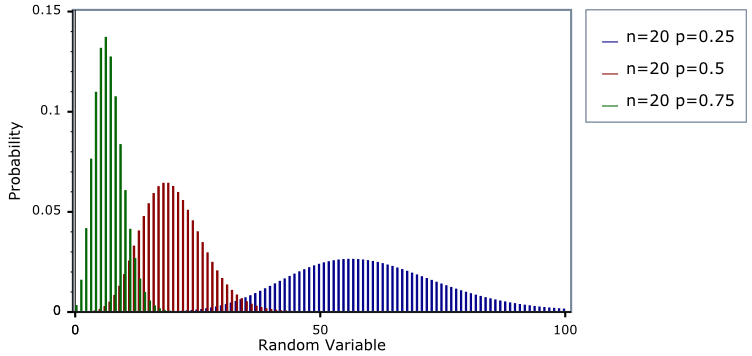
\includegraphics[width=.49\linewidth]{resources/negative_binomial_pdf_1.png}
  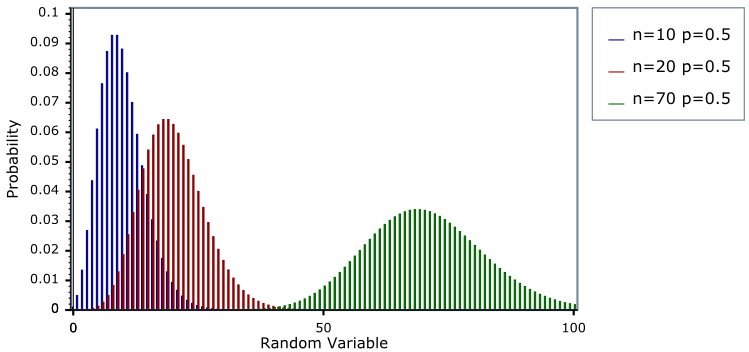
\includegraphics[width=.49\linewidth]{resources/negative_binomial_pdf_2.png}
\end{center}

\subsubsection*{The Expected Number of Successes}
The expected number of successes for $n$ Bernoulli trials with probability of success $p$ is
\[
  E[K] = np,
\]
where $K$ is the random variable denoting the number of successes in $n$ Bernoulli trials, and $E[K]$ is the expected number of successes.
\section{Graphs}
\subsection{Introduction to Graphs}
Graphs are fundamental objects in discrete mathematics that model relationships between pairs of objects. Graphs arise in a wide array of disciplines but play an especially important role in computer science.

In an \bld{undirected graph}, the edges are unordered pairs of vertices, which is useful for modeling relationships that are symmetric. A graph consists of a pair of sets $(V,E)$, where $V$ is a set of vertices and $E$ is a set of edges. A graph is \bld{finite} if the vertex set is finite. A single element of $V$ is called a \bld{vertex} and is usually represented pictorially by label, or a dot with a label. Each edge in $E$ is a set of two vertices from $V$ and is drawn as a line connecting the two vertices.
\begin{center}
  \begin{tikzpicture}
    %VARIABLES
    \pgfmathsetmacro{\gsize}{1};
    \pgfmathsetmacro{\gnum}{5};

    \foreach[count=\i] \element in {a,b,c,d,e} { %domain
        \node (\element) at (\i * 360 / \gnum:\gsize) {$\element$};
        \node (\element-) at (\i * 360 / \gnum:\gsize + 0.5) {};
      }
    \foreach \j/\l in {a/b,a/c,b/c,b/e,c/d,d/e} { %a to b
        \draw (\j) -- (\l);
      }
    \node[anchor=east] (name) at (145:\gsize+.5) {An undirected graph}; %relation name
  \end{tikzpicture}
\end{center}
In the above graph, two edges cross each other, but there is no vertex at the crossing. The crossing is just a byproduct of how the graph is drawn on a two-dimensional surface. The graph above can be described by listing the vertex set and the edge set:
\begin{align*}
  V & = \{a,b,c,d,e\}                                       \\
  E & = \{\{a,b\},\{a,c\},\{b,c\},\{b,e\},\{c,d\},\{d,e\}\}
\end{align*}
A graph may appear to be disconnected into more than one piece but is still considered to be one graph. Here are two graphs, each with 5 vertices.
\begin{center}
  \begin{tikzpicture}
    %VARIABLES
    \pgfmathsetmacro{\gsize}{1};
    \pgfmathsetmacro{\gnum}{5};

    \foreach[count=\i] \element in {a,b,c,d,e} { %domain
        \node (\element) at (\i * 360 / \gnum:\gsize) {$\element$};
        \node (\element-) at (\i * 360 / \gnum:\gsize + 0.5) {};
      }
    \foreach \j/\l in {a/b,c/d,d/e} { %a to b
        \draw (\j) -- (\l);
      }
    \node[anchor=east] (name) at (145:\gsize+.5) {Graph $A$}; %relation name
  \end{tikzpicture}
  \begin{tikzpicture}
    %VARIABLES
    \pgfmathsetmacro{\gsize}{1};
    \pgfmathsetmacro{\gnum}{5};

    \foreach[count=\i] \element in {a,b,c,d,e} { %domain
        \node (\element) at (\i * 360 / \gnum:\gsize) {$\element$};
        \node (\element-) at (\i * 360 / \gnum:\gsize + 0.5) {};
      }
    \node[anchor=east] (name) at (145:\gsize+.5) {Graph $B$}; %relation name
  \end{tikzpicture}
\end{center}
\bld{Parallel edges} are multiple edges between the same pair of vertices. In defining graphs with parallel edges, it \itl{might} be important to have additional label besides the two endpoints to specify an edge in order to distinguish between different parallel edges. A graph can also have a \bld{self-loop} which is an edge between a vertex, and itself.
\begin{center}
  \begin{tikzpicture}
    %VARIABLES
    \pgfmathsetmacro{\gsize}{1};
    \pgfmathsetmacro{\gnum}{4};

    \foreach[count=\i] \element in {a,b,c,d} { %domain
        \node (\element) at (\i * 360 / \gnum:\gsize) {$\element$};
        \node (\element-) at (\i * 360 / \gnum:\gsize + 0.5) {};
      }
    \foreach \j/\l in {a/c,b/d,c/d} { %a to b
        \draw (\j) -- (\l);
      }
    \foreach \j/\l in {a/b} { %a to b TWICE (parallel edges)
        \draw (\j) to[bend left=20 / \gsize + 10] (\l);
        \draw (\l) to[bend left=20 / \gsize + 10] (\j);
      }
    \foreach \j in {c} { %a to a
        \draw (\j) to[bend left=65] (\j-)
        to[bend left=65] (\j);
      }
    \node[anchor=east] (name) at (145:\gsize+.5) {A graph with parallel edges and a self-loop}; %relation name
  \end{tikzpicture}
\end{center}
If a graph does not have parallel edges or self-loops, it is said to be a \bld{simple graph}.

\subsubsection*{Graph terminology}
\begin{center}
  \begin{tikzpicture}
    %VARIABLES
    \pgfmathsetmacro{\gsize}{1};
    \pgfmathsetmacro{\gnum}{5};

    \foreach[count=\i] \element in {a,b,c,d,e} { %domain
        \node (\element) at (\i * 360 / \gnum:\gsize) {$\element$};
        \node (\element-) at (\i * 360 / \gnum:\gsize + 0.5) {};
      }
    \foreach \j/\l in {a/b,a/c,b/c,b/e,c/d,d/e} { %a to b
        \draw (\j) -- (\l);
      }
    \node[anchor=east] (name) at (145:\gsize+.5) {Undirected graph example}; %relation name
  \end{tikzpicture}
\end{center}
\begin{itemize}
  \item If there is an edge between two vertices, they are said to be \bld{adjacent}. In the graph above, $d \tand e$ are adjacent, but $d \tand b$ are not adjacent.
  \item Vertices $b \tand e$ are the \bld{endpoints} of edge $\{b,e\}$. The edge $\{b,e\}$ is \bld{incident} to vertices $b tand e$.
  \item A vertex $c$ is a \bld{neighbor} of vertex $b$ if and only if $\{b,c\}$ is an edge. In the graph above, the neighbors of $b$ are the vertices $a,c, \tand e$.
  \item In a simple graph, the \bld{degree} of a vertex is the number of neighbors it has. In the graph above, the degree of $b$ is 3 and the degree of vertex $a$ is 2. The degree of vertex $b$ is denoted by $\deg(b)$.
  \item The \bld{total degree} of a graph is the sum of the degrees of all of the vertices. The total degree of the above graph is $2 + 3 + 3 + 2 + 2 = 12$.
  \item In a \bld{regular graph}, all the vertices have the same degree. In a \bld{$d$-regular graph}, all the vertices have degree $d$. The graph above is not regular because $\deg(a) \neq \deg(b)$. However, the graph below is 3-regular.
\end{itemize}
\begin{center}
  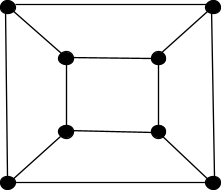
\includegraphics[width=.2\linewidth]{resources/3-regular graph.png}
\end{center}
\begin{itemize}
  \item A graph $H = (V_H,E_H)$ is a \bld{subgraph} of a graph $G = (V_G,E_G)$ if $V_H \subseteq V_G \tand E_H \subseteq E_G$. Note that any graph $G$ is a subgraph of itself.
\end{itemize}
\begin{center}
  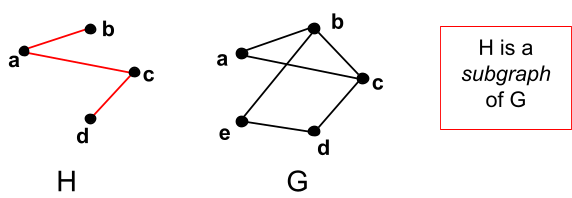
\includegraphics[width=.6\linewidth]{resources/H is a subgraph of G.png}
\end{center}

\subsubsection*{Theorem: Number of Edges and Total Degree}
Let $G = (V,E)$ be an undirected graph, simple or not. Then, twice the number of edges is equal to the total degree:
\[
  \sum_{v \in V} \deg(v) = 2 \cdot |E|
\]

\subsubsection*{Common Graphs}
Some graphs with special structure are given their own name and notation because they come up so frequently in graph theory.
\begin{center}
  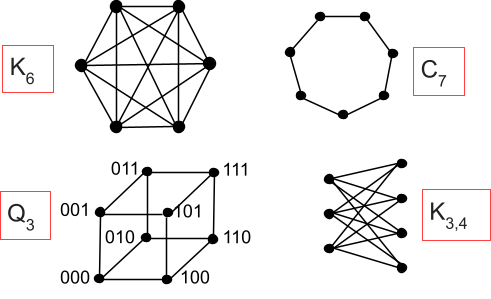
\includegraphics[width=0.6\linewidth]{resources/common graphs.png}
\end{center}
For the definition of all of these graphs, $n \in \bb{Z}^+$.
\begin{itemize}
  \item $K_n$ is called the \bld{complete graph} on $n$ vertices. $K_n$ has an edge between every pair of vertices. $K_n$ is sometimes called a \bld{clique} of size $n$ or an \bld{$n$-clique}.
  \item $C_n$ is called a cycle on $n$ vertices. The edges connect the vertices in a ring. Note that $C_n$ is well defined only for $n \geq 3$.
  \item The $n$-dimensional hypercube, denoted $Q_n$, has $2^n$ vertices. Each vertex is label with an $n$-bit string. Two vertices are connected by an edge if their corresponding labels differ only by one bit.
  \item $K_{n,m}$ has $n+m$ vertices, and $2nm$ edges. The vertices are divided into two sets: one with $m$ vertices and one set with $n$ vertices. There are no edges between vertices in the same set, but there is an edge between every vertex in one set and every vertex in the other set.
\end{itemize}

\subsection{Graph representations}
\begin{center}
  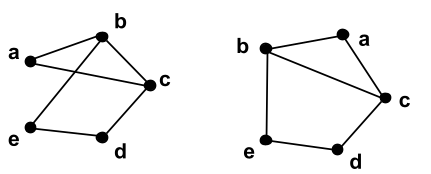
\includegraphics[width=0.5\linewidth]{resources/two similar graphs.png}
\end{center}
These two graphs look different, but that is only because they are drawn differently. The two graphs are actually the same graph because they have the same vertex and edge sets as shown below:
\begin{align*}
  V & = \{a,b,c,d,e\}                                       \\
  E & = \{\{a,b\},\{a,c\},\{b,c\},\{b,e\},\{c,d\},\{d,e\}\}
\end{align*}
The way a graph is drawn is not part of the graph itself.

\subsubsection*{Adjacency List Representation for Graphs}
In the \bld{adjacency list representation} of a graph, each vertex has a list of all its neighbors. Note that since the graph is undirected if vertex $a$ is in $b$'s list of neighbors, then $b$ must also be in $a$'s list of neighbors.

If a graph is represented using adjacency lists, the time required to list the neighbors of a vertex $v$ is proportional to $\deg(v)$, the number of vertices to be listed. In order to determine if $\{a,b\}$ is an edge, it is necessary to scan the list of $a$'s neighbors or the list of $b$'s neighbors. In the worst case, the time required is proportional to the larger of $\deg(a)$ or $\deg(b)$.

\subsubsection*{Matrix Representation for Graphs}
The \bld{matrix representation} for a graph with $n$ vertices is an $n \times n$ matrix whose entries are all either $0 \tor 1$, indicating whether or not each edge is present. The matrix representation of an undirected graph is symmetric.
\begin{center}
  \begin{tikzpicture}
    %VARIABLES
    \pgfmathsetmacro{\gsize}{1};
    \pgfmathsetmacro{\gnum}{5};

    \foreach[count=\i] \element in {a,b,c,d,e} { %domain
        \node (\element) at (\i * 360 / \gnum:\gsize) {$\element$};
        \node (\element-) at (\i * 360 / \gnum:\gsize + 0.5) {};
      }
    \foreach \j/\l in {a/b,a/c,b/c,b/e,c/d,d/e} { %a to b
        \draw (\j) -- (\l);
      }
    \node[anchor=east] (name) at (145:\gsize+.5) {}; %relation name
  \end{tikzpicture} $~~\Rightarrow~~$
  $
    \begin{bmatrix}
      0 & 1 & 1 & 0 & 0 \\
      1 & 0 & 1 & 0 & 1 \\
      1 & 1 & 0 & 1 & 0 \\
      0 & 0 & 1 & 0 & 1 \\
      0 & 1 & 0 & 1 & 0
    \end{bmatrix}
  $
\end{center}

\subsection{Graph isomorphism}
Two graphs are said to be \bld{isomorphic} if there is a correspondence between the vertex sets of each graph such that there is an edge between two vertices of one graph if and only if there is an edge between the corresponding vertices of the second graph. Essentially, the graphs are not identical but the vertices can be relabeled so that they are identical.

\subsubsection*{Definition of Isomorphic Graphs}
Let $G = (V,E) \tand G'=(V',E')$. $G \tand G'$ are isomorphic if there is a bijection $f: V \rightarrow V'$ such that for every pair of vertices $x,y \in V$, $\{x,y\} \in E$ if and only if $\{f(x), f(y)\} \in E'$. The function $f$ is called an \bld{isomorphism} from $G \tto G'$.

\begin{center}
  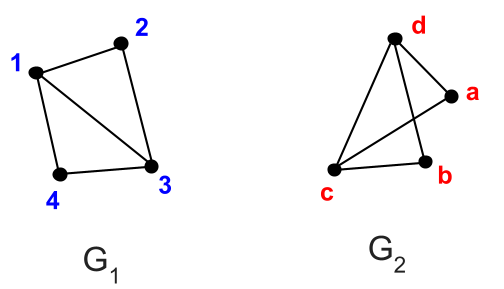
\includegraphics[width=0.4\linewidth]{resources/isomorphic graphs 1.png}
\end{center}
The following function is an isomorphism from the vertices of $G_1 \tto G_2$:
\[
  f(1) = d \qquad f(2) = a \qquad f(3) = c \qquad f(4) = b
\]

\subsubsection*{Theorem: Vertex Degree Preserved under Isomorphism}
Consider two graphs, $G \tand G'$. Let $f$ be an isomorphism from $G \tto G'$. For each vertex $v \tin G$, the degree of vertex $v \tin G$ is equal to the degree of vertex $f(v) \tin G'$.

\subsubsection*{}
The \bld{degree sequence} of a graph is a list of the degree of all of the vertices in non-increasing order.
\begin{center}
  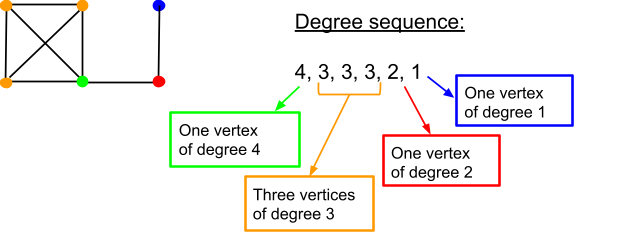
\includegraphics[width=0.7\linewidth]{resources/degree-sequence.png}
\end{center}

\subsubsection*{Theorem: Degree Sequence Preserved under Isomorphism}
The degree sequence of a graph is preserved under isomorphism.


\subsection{Walks, trails, circuits, paths, and cycles}
A \bld{walk} from $v_0 \tto v_l$ in an undirected graph $G$ is a sequence of alternating vertices and edges that starts and ends with a vertex:
\[
  \langle v_0,\{v_0,v_1\},v_1,\{v_1,v_2\},\ldots,v_{\ell-1},\{v_{\ell-1},v_\ell\},v_\ell\rangle
\]
Since the edges in a walk are completely determined by the vertices, a walk can also be denoted by the sequence of vertices:
\[
  \langle v_0,v_1,\ldots,v_\ell \rangle.
\]
However, keep in mind the sequence of vertices is a walk only if $\{v_{j-1},v_j\} \in E$ for each $j = 1,2,\ldots,\ell$. The \bld{length of a walk} is $\ell$, the number of edges in the walk. An \bld{open walk} is a walk in which the first and last vertices are not the same. A \bld{closed walk} is a walk in which the first and last vertices are the same.
\begin{itemize}
  \item A \bld{trail} is a walk in which no \itl{edge} occurs more than once.
  \item A \bld{path} is a walk in which no \itl{vertex} occurs more than once.
  \item A \bld{circuit} is a closed \itl{trail}.
  \item A \bld{cycle} is a \itl{circuit} is length at least 1 in which no vertex occurs more than once, except the first and last vertices which are the same.
\end{itemize}
Here are some examples of closed walks:
\begin{itemize}
  \item $\langle A,C,D,A \rangle$ is a \itl{trail}, a \itl{circuit}, and a \itl{cycle}.
  \item $\langle A,C,B,A,D,E,A \rangle$ is a \itl{trail} and a \itl{circuit}.
  \item $\langle A,B,A \rangle$ is \bld{not} a trail, circuit, or a cycle.
\end{itemize}
Since paths and cycles do not have any repeated edges, if a graph is simple, any cycle \itl{must} have length at least 3. The sequence $\langle v \rangle$ is not a cycle because a cycle, by definition, must have length at least 1. The sequence $\langle v,v \rangle$ is only a walk if there is a self-loop at vertex $v$.

\subsection{Graph connectivity}
Two vertices, $v \tand w$, are \bld{connected} if there is a path from $v \tto w$ (and thus also a path from $w \tto v$). A vertex is always considered to be connected to itself. The property of being connected can be extended to sets of vertices and the entire graph:
\begin{itemize}
  \item A set of vertices in a graph is said to be connected if every pair of vertices in the set is connected.
  \item A graph is said to be connected if every pair of vertices in the graph is connected, and is \bld{disconnected} otherwise.
\end{itemize}
A \bld{connected component} consists of a \itl{maximal} set of vertices that are connected as well as all the edges between two vertices in the set. A vertex that is not connected with any other vertex is called an \bld{isolated vertex} and is therefore a connected component with only one vertex.
\begin{center}
  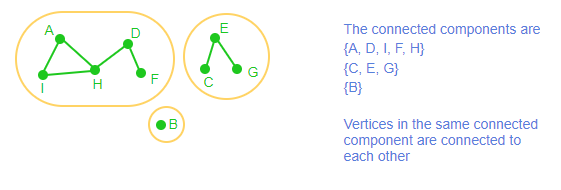
\includegraphics[width=0.6\linewidth]{resources/connected components example.png}
\end{center}

\subsubsection*{k-Connectivity}
In some networks, it is important to be able to guarantee connectivity, even if one or more vertices or edges are removed from a graph. The definition of connectivity can be extended to encompass resilience to vertex or edge failures.

\subsubsection*{Definition of a K-vertex-connected Graph}
An undirected graph $G$ is \bld{$k$-vertex-connected} if the graph contains at least $k + 1$ vertices and remains connected after any $k - 1$ vertices are removed from the graph. The \bld{vertex connectivity} of a graph is the largest $k$ such that the graph is $k$-vertex-connected. The vertex connectivity of a graph $G$ is denoted $\kappa(G)$.

The vertex connectivity of a graph is the minimum number of vertices whose removal disconnects the graph into more than one connected component.

When the graph is a complete graph, there is no set of vertices whose removal disconnects the graph. For the special case of $K_n$, the vertex connectivity $\kappa(K_n)$ is just defined to be $n - 1$.

\subsubsection*{Definition of a K-edge-connected Graph}
An undirected graph G is \bld{$k$-edge-connected} if removing any $k - 1$ or fewer edges results in a connected graph. The \bld{edge connectivity} of a graph is the largest $k$ such that the graph is $k$-edge-connected. The edge connectivity of a graph G is denoted $\lambda(G)$.

The edge connectivity of a graph is the minimum number of edges whose removal disconnects the graph into more than one connected component.

\subsubsection*{Theorem: Upper bound for Vertex and Edge Connectivity}
Let $G$ be an undirected graph. Denote the minimum degree of any vertex in $G$ by $\delta(G)$. Then,
\begin{align*}
  \kappa(G)  & \leq \delta(G)~~~\tand \\
  \lambda(G) & \leq \delta(G).
\end{align*}

\subsection{Euler circuits and trails}
An \bld{Euler circuit} is a circuit that contains every edge and every vertex. Note that a circuit, by definition, has no repeated edges, so an Euler circuit contains each edge exactly once.
\begin{center}
  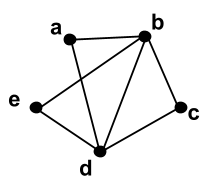
\includegraphics[width=0.2\linewidth]{resources/euler circuit example.png}
  Euler circuit: $\langle a,b,c,d,e,b,d,a \rangle$
\end{center}

\subsubsection*{Theorem: Characterization of Graphs that have an Euler Circuit}
An undirected graph $G$ has an Euler circuit if and only if $G$ is connected and every vertex in $G$ has even degree.
\[
  G~\text{has an Euler circuit}~\leftrightarrow G~\text{is connected and every vertex in $G$ has even degree}.
\]

\subsubsection*{Procedure to find a circuit in a Graph}
\begin{lstlisting}
Find a vertex w, that is not an isolated vertex.
Select any edge {w,x} incident to w.
(Since w is not isolated, there is always at least one such edge.)
Current trail T := <w,x>
last := x
While there is an edge {last, y} that has not been used in T:
  Add y to the end of T
  last := y
\end{lstlisting}

\subsubsection*{Procedure to find an Euler circuit in a Graph}
Use the procedure above to find any circuit in $G$. Call the circuit $C$. The algorithm continues to iterate the following steps until all the edges in $G$ are included in $C$:
\begin{enumerate}
  \item Remove all edges in $C$ from $G$. Remove any isolated vertices from $G$. Call the resulting graph $G'$.
  \item Find a vertex $w$ that is in $G' \tand C$.
  \item Find a circuit in $G'$ that begins and ends with $w$. Call the circuit $C'$.
  \item Combine circuit $C \tand C'$. Suppose $C$ starts and ends at vertex $v$. Create a new circuit that starts at $v$ and follows the edges in $C$ until $w$ is reached. The new circuit then follows the edges in $C'$ back to $w$ and then follows the rest of the edges in $C$ back to $v$. The new circuit is renamed $C$ for the next iteration.
\end{enumerate}


\subsubsection*{Euler trail}
An \bld{Euler trail} is an open trail that includes each edge. Note that a trail, by definition, has no repeated edges, so an Euler trail contains each edge exactly once. In an open trail, the first and last vertices are not equal.

\subsubsection*{Theorem: Characterizations of graphs that have an Euler trail}
An undirected graph $G$ has an Euler trail if and only if $G$ is connected and has exactly two vertices with odd degree. The Euler trail begins and ends with the vertices of odd degree.
\[
  G~\text{has an Euler trail}~\leftrightarrow G~\text{is connected and has exactly two vertices with odd degree}.
\]

\subsection{Hamiltonian cycles and paths}
A \bld{Hamiltonian cycle} in an undirected graph is a cycle that includes every vertex in the graph. Note that a cycle, by definition, has no repeated vertices or edges, except for the vertex which is at the beginning and end of the cycle. Therefore, every vertex in the graph appears exactly once in a Hamiltonian cycle, except for the vertex which is at the beginning and end of the cycle. A \bld{Hamiltonian path} in an undirected graph is a path that includes every vertex in the graph. Note that a path, by definition, has no repeated vertices or edges, so every vertex appears exactly once in a Hamiltonian path.

Note that a Hamiltonian cycle can be transformed into a Hamiltonian path by deleting the last vertex. Therefore if a graph has a Hamiltonian cycle, then the graph also has a Hamiltonian path.

Unlike Euler circuits and trails, there are no known conditions describing exactly which graphs have a Hamiltonian cycle or path. However, there are some cases in which a graph that does have a Hamiltonian cycle or path has a certain property.
\begin{itemize}
  \item Any graph that has a vertex with degree 1 does not have a Hamiltonian cycle.
  \item For $n \geq 3$, $K_n$ has a Hamiltonian cycle.
\end{itemize}

\subsection{Planar graphs}
Placing graphs on two-dimensional surfaces to avoid crossings is a classic problem in graph theory. The problem also arises in the field of graph drawing in which the goal is to draw complex graphs in a way that helps people visualize structure and patterns.

An \bld{embedding} for $G = (V,E)$ is an assignment of the vertices to points in the plane and an assignment of each edge to a continuous curve. The curve for each edge must start and edge at the two points corresponding to the endpoints of the edge. Essentially, an \itl{embedding is a way of drawing a graph} on a plane, because mathematically, a graph is just a set of vertices and a set of edges.

An embedding is said to be a \bld{planar embedding} if none of the edges cross. There is a crossing between two edges in an embedding if their curves intersect at a point that is not a common endpoint. An embedding of a graph can be planar or not planar, depending on whether it has a crossing. Planarity can also be defined as a property of the graph itself.

\subsubsection*{Definition of Planar Graphs}
A graph $G$ is a \bld{planar graph} if the graph has a planar embedding.

\begin{center}
  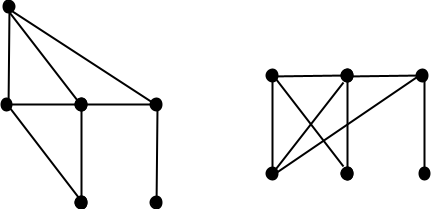
\includegraphics[width=0.4\linewidth]{resources/two embeddings.png}
\end{center}
\begin{itemize}
  \item The embedding on the left \itl{is planar}.
  \item The embedding on the right \itl{is \bld{not} planar}.
\end{itemize}

The \bld{complement of an embedding} is the set of all points in the plane that are not part of a curve corresponding to an edge. A planar embedding carves up the plane into continuous regions. A \bld{region} is a set of points in the complement of an embedding that forms a maximal continuous set, meaning that it is (continuous): possible to travel anywhere from any point in the region and (maximal): if any point were added to the region, it would no longer be continuous. In a planar embedding, there is always an infinite region called the \bld{exterior region}, which is region $V$ in the following graph.
\begin{center}
  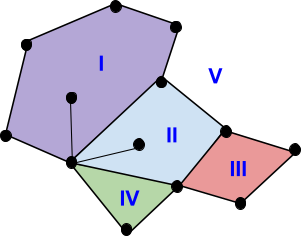
\includegraphics[width=0.4\linewidth]{resources/regions of a planar embedding.png}
\end{center}

\subsubsection*{Theorem: Euler's Identity for Regions in an Embedding}
Consider a planar embedding of a connected graph $G$. Let $v$ be the number of vertices in $G$, $e$ the number of edges, and $r$ the number of regions in the embedding. Then,
\[
  v - e + r = 2
\]

\subsubsection*{Degree of a Region}
\begin{center}
  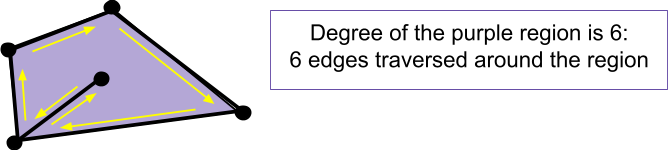
\includegraphics[width=0.6\linewidth]{resources/degree of a region.png}
\end{center}
Consider a planar embedding of a graph G. Think of a tiny bug walking all the way around the region along the edges of the graph. The degree of a region is the number of times the bug traverses an edge until it gets back to its starting location. Note that if an edge sticks out into a region, the edge can be traversed twice by the bug and therefore contributes 2 towards the degree of the region.

\subsubsection*{Theorem: Number of Edges in a Planar Graph}
Let G be a connected planar graph. Let $v$ be the number of vertices in G and $e$ the number of edges. If $v \geq 3$, then
\[
  e \leq 3v-6
\]

\subsection{Graph coloring}
Graph coloring is a classic problem in graph theory because it is useful in modeling resource constraints like scheduling.

\subsubsection*{Definition of Graph Coloring}
Let $G=(V,E)$ be an undirected graph and $C$ a finite set of colors. A \bld{valid coloring} of $G$ is a function $f: V \rightarrow C$ such that for every edge $\{x,y\} \in E, f(x) \neq f(y)$. If the size of the range of function $f$ is $k$, then $f$ is called a \bld{$k$-coloring} of $G$.

\subsubsection*{}
The coloring on the left is a valid coloring because no two adjacent vertices are assigned the same color. The coloring on the left is a 3-coloring because 3 colors are used. The coloring on the right is not a valid coloring because there is an edge whose endpoints are both colored pink.
\begin{center}
  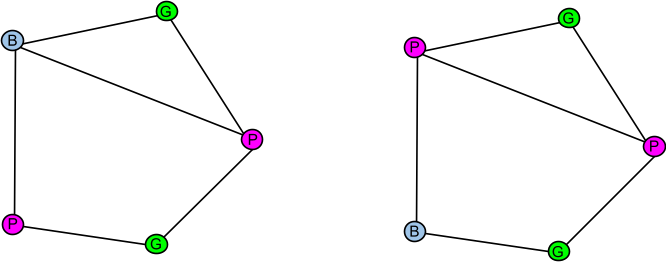
\includegraphics[width=0.5\linewidth]{resources/graph colorings.png}
\end{center}

\subsubsection*{Definition of the Chromatic Number of a Graph}
The \bld{chromatic number} of a graph $G$, denoted as $X(G)$ is the smallest $k$ such that there is a valid $k$-coloring of $G$. It is minimum number of colors that a graph requires to have a valid graph coloring.

\subsubsection*{}
In general, if $K_r$ is a subgraph of $G$, then there is a subset of $r$ vertices in $G$ such that every pair of vertices in the subset is connected by an edge. In any valid coloring of $G$, each of the $r$ vertices in the subset must be assigned a distinct color which implies that $X(G) \geq r$. The clique number of a graph G, denoted $\omega(G)$, is the largest $r$ such that $K_r$ is a subgraph of $G$.

\subsubsection*{Theorem: Relationship between the Clique Number of Chromatic Number}
If $G$ is an undirected graph, then
\[
  \omega(G) \leq X(g)
\]

\subsubsection*{Greedy coloring}
In general, it is difficult to determine the chromatic number of a graph $G$. However, there is an easy and natural method to color the vertices of a graph called the \itl{greedy coloring algorithm}. The \bld{greedy coloring algorithm} often leads to a color that uses a small number of colors, but there is no guarantee that it uses the \itl{smallest} number of colors possible for a given graph.

\subsubsection*{The Greedy Coloring Algorithm}
\begin{enumerate}
  \item Number the set of possible colors. Assume that there is a very large supply of different colors, even though they might not all be used.
  \item Order to vertices in any arbitrary order.
  \item Consider each vertex $v$ in order. Assign $v$ a color that is different from the color of $v$'s neighbors that have already been assigned that color. When selecting a color for $v$, use the lowest number color possible.
\end{enumerate}
The term "greedy" is used to describe a general paradigm for solving many different kinds of problems. Greedy algorithms typically solve a problem one piece at a time.

The greedy algorithm provides a way to upper bound the chromatic number of a graph.

\subsubsection*{Theorem: Upper bound for $X(G)$}
Let $G$ be an undirected graph. Let $\Delta(G)$ be the maximum degree of any vertex in $G$. Then,
\[
  X(G) \leq \Delta(G)+1
\]
\section{Trees}
\subsection{Introduction to trees}
\begin{center}
  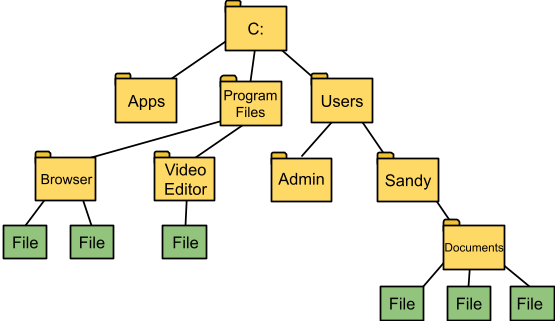
\includegraphics[width=0.6\linewidth]{resources/diagram of a file system.png}
\end{center}
The file system can be seen as a graph in which each folder or file is a vertex. There is an edge between two folders if one folder is a subfolder of the other. There is an edge between a file and a folder if the file resides in that folder. In most computer operating systems, a file or folder can only reside in one location, which means that the underlying graph corresponds to a tree.

\subsubsection*{Definition of a Tree}
A \bld{tree} is an undirected graph that is connected and has no cycles.

\subsubsection*{Free Trees and Rooted Trees}
\begin{center}
  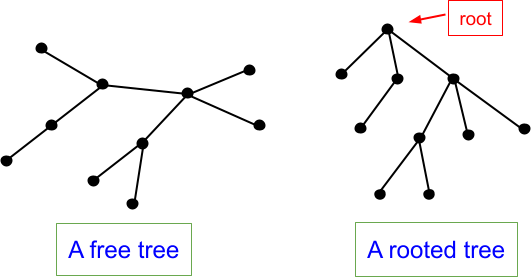
\includegraphics[width=0.5\linewidth]{resources/free and rooted trees.png}
\end{center}
The tree on the left is called a \bld{free tree} because there is no particular organization of the vertices and edges. The tree on the right is called a \bld{rooted tree}. The vertex at the top of the drawing is designated as the \bld{root} of the tree. The remaining vertices are organized according to their distance from the root. The distance between two vertices in an undirected graph is the number of edges in the shortest path between the two vertices. The \bld{level} of a vertex is its distance from the root. The \bld{height} of a tree is the highest level of any vertex. The tree on the right has height 3.

\subsubsection*{Theorem: Unique Paths in Trees}
Let $T$ be a tree and let $u \tand v$ be two vertices in $T$. There is \itl{exactly one path} between $u \tand v$.

\subsubsection*{Terminology related to Rooted Trees}
\begin{itemize}
  \item Every vertex in a rooted tree $T$ has a unique \bld{parent}, except for the root which does not have a parent. The parent of vertex $v$ is the first vertex encountered along the path from $v$ to the root.
  \item Every vertex along the path from $v$ to the root, except for the vertex $v$ itself, is an \bld{ancestor} of vertex $v$.
  \item If $v$ is the parent of vertex $u$, then $u$ is a \bld{child} of vertex $v$.
  \item If $u$ is an ancestor of $v$, then $v$ is a \bld{descendant} of $u$.
  \item A \bld{leaf} is a vertex which has no children.
  \item Two vertices are \bld{siblings} if they have the same parent.
  \item A \bld{subtree} rooted as vertex $v$ is the tree consisting of $v$ and all of $v$'s descendants.
\end{itemize}

\subsubsection*{Forests}
A \bld{forest} is a graph that has no cycles but is not necessarily connected. The picture below shows a forest with 3 connected components.
\begin{center}
  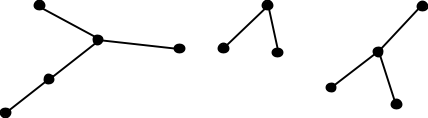
\includegraphics[width=0.6\linewidth]{resources/forest example.png}
\end{center}

\subsection{Tree application examples}

\subsubsection*{Game Trees}
\begin{center}
  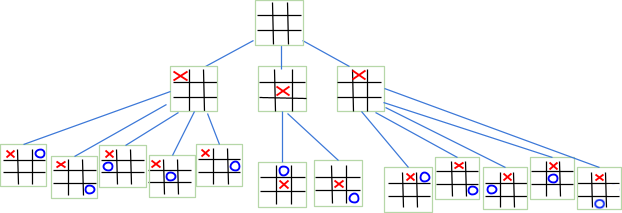
\includegraphics[width=0.7\linewidth]{resources/tictactoe game tree.png}
\end{center}
The root of the tree is the initial configuration of the game. In the case of tic-tac-toe, the initial configuration is an empty grid. The odd levels of the game tree represent choices of play for the X player and the even levels represent choices of play for the O player. The children of a configuration c are all the configurations that can be reached from c by a single move of the correct player. A configuration is a leaf vertex in the tree if the game is over.

Theoretically, a game tree can be systematically analyzed to determine optimal playing strategies for each player. However, in practice for most games, the corresponding game tree is much too large to build and analyze in its entirety. Programs like Deep Blue build partial game trees starting from the current configuration in the game and estimate the best next move based on the results of the partial tree.

Tic-tac-toe and chess are examples of deterministic games whose outcome is completely determined by the choices made by each player. A game that involves rolling a pair of dice or shuffling a deck of cards introduces randomization into the game. Probability theory as well as game trees are required to analyze games with an element of chance.

\subsubsection*{Prefix Codes}
Space-efficient encodings can be achieved by \bld{variable length codes}, in which the number of bits for each character can vary. Characters such as "a" and "e" that occur frequently are represented with fewer bits, while characters such as "z" or "q" are represented using more bits.

Trees are a convenient way to represent variable length codes for translating between text and binary.
\begin{center}
  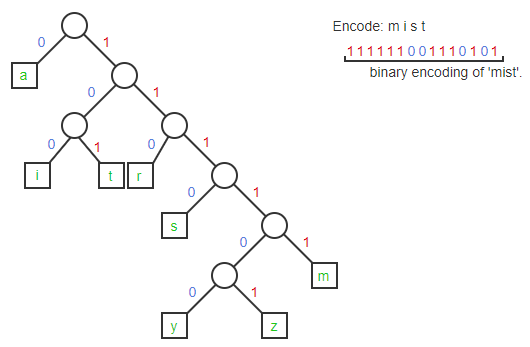
\includegraphics[width=0.6\linewidth]{resources/variable length encoding example.png}
\end{center}
The code illustrated in the animation is an example of a prefix code. A string $s$ is a \bld{prefix} of another string $t$ if all the characters in string $s$ appear at the beginning of string $t$.
\begin{center}
  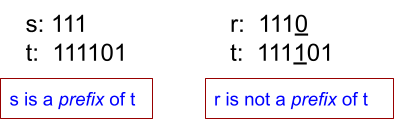
\includegraphics[width=0.4\linewidth]{resources/string prefix example.png}
\end{center}
A \bld{prefix code} has the property that the code for one character \itl{can not} be a prefix of the code for another character. The fact that the codes are organized as a tree in which characters are only stored at the leaves ensures the prefix property.

\subsection{Properties of trees}

\subsubsection*{Theorem: Unique Paths in Trees}
There is a unique path between every pair of vertices in a tree.

\subsubsection*{Theorem: Number of Leaves in a Tree}
Any free tree with at least two vertices has at least two leaves.

\subsubsection*{Theorem: Number of Edges in a Tree}
Let $T$ be a tree with $v$ vertices and $e$ edges. Then
\[
  e = v-1.
\]

\subsection{Tree traversals}
A common procedure performed on a tree, called a \bld{tree traversal}, is to process the information stored in the vertices by systematically visiting each vertex. In a \bld{pre-order traversal}, a vertex is visited before its descendants. In a \bld{post-order traversal}, a vertex is visited after its descendants.

\subsubsection*{Pseudocode and Example for Pre-order Traversal}
\begin{lstlisting}
Pre-order(v)

process(v) // process happens first
For every child w of v:
  Pre-order(w)
End-for
\end{lstlisting}
\begin{center}
  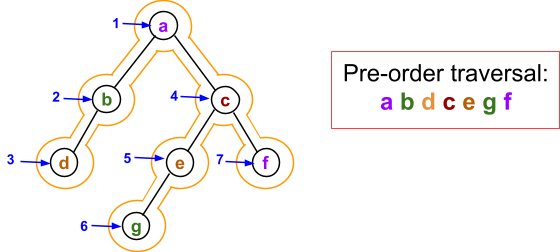
\includegraphics[width=0.4\linewidth]{resources/preorder traversal.png}
\end{center}

\subsubsection*{Pseudocode and Example for Post-order Traversal}
\begin{lstlisting}
Post-order(v)

For every child w of v:
  Post-order(w)
End-for
process(v) // process happens last
\end{lstlisting}
\begin{center}
  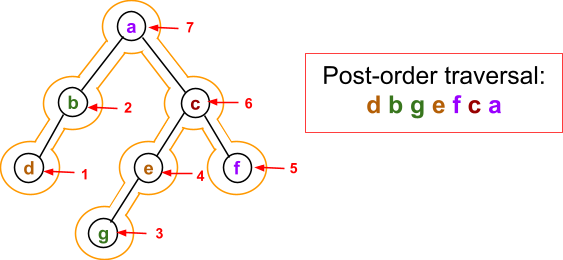
\includegraphics[width=0.4\linewidth]{resources/post order traversal.png}
\end{center}

\subsection{Spanning trees and graph traversals}
Suppose an application needs to broadcast information to every computer (vertex) in a network. The information will be disseminated along the communication links so that every vertex in the network receives the information. Moreover, the goal is to minimize overall congestion, so it would be wasteful to send information along alternate paths to the same location. The information should be broadcast over a spanning tree of the network. Here is the formal definition of a spanning tree:

\subsubsection*{Definition of a Spanning Tree of a Connected Graph}
A \bld{spanning tree} of a connected graph $G$ is a subgraph of $G$ which contains all the vertices in $G$ and is a tree.

\subsubsection*{}
The picture below shows several possible spanning trees of the same graph. The edges of the spanning tree are shown in red. The vertex set of the spanning tree is always the entire set of vertices in the graph.
\begin{center}
  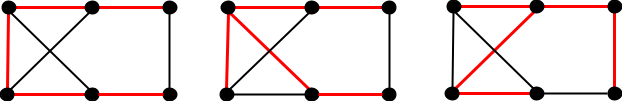
\includegraphics[width=0.6\linewidth]{resources/spanning trees example.png}
\end{center}

\subsubsection*{Graph Traversals}
There are two common methods for finding spanning trees in a graph: Breadth-First Search and Depth-First Search. Both methods start at a single vertex and incrementally build a connected tree by adding edges and vertices. The resulting tree is rooted at the start vertex. Graph traversal is a process that systematically explores all the vertices of a graph.

\subsubsection*{Depth-First Search}
As the name suggests, Depth-First Search (DFS) favors going deep into the graph and tends to produce trees with longer paths from the start vertex.
\begin{lstlisting}
Depth-first-search

Input: An undirected, connected graph G. A start vertex v[1]
Output: T, a depth-first search tree.

Add v[1] to T.
visit(v[1])

visit(v)

For every neighbor w of v:
  If w is not already in T
    Add w and {w, v} to T.
    visit(w);
  End-if
End-for
\end{lstlisting}
Note that there is some ambiguity with regard to the order in which the neighbors of a vertex are considered.

\subsubsection*{Breath-first Search}
Breadth-First Search (BFS) explores the graph by distance from the initial vertex, starting with its neighbors and expanding the tree to neighbors of neighbors, etc. Breadth-first-search visits vertices in the graph according to their proximity to the start vertex. The algorithm maintains a list of vertices to be visited soon. Vertices are added to the back of the list and the next vertex to visit is taken from the front of the list.
\begin{lstlisting}
Breadth-first-search

Input: An undirected, connected graph G. A start vertex v[1]
Output: T, a breadth-first search tree.

Add v[1] to T.
Add v[1] to the back of the list.

While the list is not empty:
  Remove vertex v from the front of the list.
  For each neighbor w of v that is not already in T:
    Add w and {w, v} to T.
    Insert w at the back of the list.
  End-for
End-while
\end{lstlisting}

\subsection{Minimum spanning trees}
When edges have varying costs, a natural goal is to minimize the total cost of the spanning tree.

\subsubsection*{Definition of a Weighted Graph}
A \bld{weighted graph} is a graph $G = (V,E)$, along with a function $w: E \rightarrow \bb{R}$. The function $w$ assigns a real number to each edge.
\begin{center}
  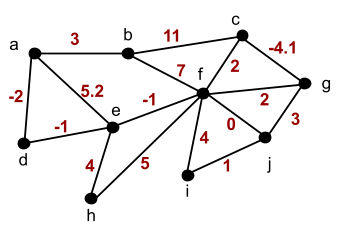
\includegraphics[width=0.6\linewidth]{resources/example weighted graph.png}
\end{center}
When the goal is to span the vertices of the graph while minimizing the total weight of the edges used, a \bld{minimum spanning tree} can be used.

\subsubsection*{Definition of a Minimum Spanning Tree}
A \bld{minimum spanning tree} (MST) of a weighted graph is a spanning tree $T$ of $G$ whose weight is no larger than any other spanning tree of $G$.

\subsubsection*{Prim's Algorithm for Minimum Spanning Trees}
This is a classic algorithm for finding minimum spanning trees, developed by mathematician Robert Prim in 1957.
\begin{lstlisting}
Input: An undirected, connected, weighted graph G.
Output: T, a minimum spanning tree for G.

T := {}.
Pick any vertex in G and add it to T.

For j = 1 to n-1
  Let C be the set of edges with one endpoint inside T 
      and one endpoint outside T.
  Let e be a minimum weight edge in C.
  Add e to T.
  Add the endpoint of e not already in T to T.
End-for
\end{lstlisting}

\subsubsection*{Theorem: Result of Prim's Algorithm}
Prim's algorithm finds a minimum spanning tree of the input weighted graph.

\end{document}